\section*{第四章 参数方程、极坐标}

1. D 提示: 参数方程化为普通方程时,不能任意缩小或扩大曲线中 $x$ , $y$ 的取值范围. 普通方程 ${xy} = 1$ 中, $x,y \in  \mathbf{R}$ 且 $x,y \neq$ 0. 对于 $\left( A\right) ,x,y$ 是正数; 对于 $\left( B\right) ,x \in  \left\lbrack  {-1,1}\right\rbrack$ 且 $x \neq  0,y \in  \left( {-\infty , - 1}\right\rbrack   \cup  \lbrack 1, + \infty )$ ; 对于 $\left( C\right) ,x \in  \left\lbrack  {-1,1}\right\rbrack$ 且 $x \neq  0,y \in$  $\left( {-\infty , - 1\rbrack \cup \lbrack 1, + \infty }\right)$ ,对于 (D), $x,y \in  \mathbf{R}$ 且 $x,y \neq  0$ ,且 $x \cdot  y = \tan t \cdot  \cot t = 1$ ,与普通方程一致.

2. D 提示: $x = 1 + \cos {2\theta } = 1 + \left( {1 - 2{\sin }^{2}\theta }\right) ,\therefore x = 2 - {2y}$ ,即 $x + {2y} - 2 = 0$ . 其中, $\cos {2\theta } \in  \left\lbrack  {-1,1}\right\rbrack$ ,故 $x \in  \left\lbrack  {0,2}\right\rbrack$ . 当 $x$  $= 0$ 时 $y = 1$ ; 当 $x = 2$ 时, $y = 0$ . 因此,原参数方程的轨迹是以 $\left( {2,0}\right) ,\left( {0,1}\right)$ 为端点的线段.

3. $B$ 提示: 令 $y = {t}^{2} - t = 0$ ,解得 ${t}_{1} = 0,{t}_{2} = 1$ ,代入 $x = t - 8$ ,得到 ${x}_{1} =  - 8,{x}_{2} =  - 7$ ,因此曲线与 $x$ 轴的交点坐标为 $( - 8$ , $0)$ 和(-7,0).

4. A 提示: 先化参数方程为普通方程: ${x}^{2} = {\left( \sin \theta  + \cos \theta \right) }^{2} = 1 + 2\sin \theta \cos \theta ,\;\therefore {x}^{2} = 1 + {2y}$ ,即 $y = \dfrac{1}{2}{x}^{2} - \dfrac{1}{2}$ . 再看 $x,y$ 的取值范围: $x = \sin \theta  + \cos \theta  = \sqrt{2}\sin \left( {\theta  + \dfrac{\pi }{4}}\right)  \in  \left\lbrack  {-\sqrt{2},\sqrt{2}}\right\rbrack$ ,因此原参数方程应是抛物线 $y = \dfrac{1}{2}{x}^{2} - \dfrac{1}{2}$ (开口向上,顶点为 $\left( {0, - \dfrac{1}{2}}\right)$ ) 在 $x \in  \left\lbrack  {-\sqrt{2},\sqrt{2}}\right\rbrack$ 的一段.

5. D 提示: 通过配方,得 ${\left( x - 2t\right) }^{2} + {\left( y - t\right) }^{2} = 2{t}^{2} + 4\left( {t\text{ 为参数 }}\right)$ ,其圆心为(2t, t),且 $t \in  \mathbf{R}$ . 易知,圆心轨迹在直线 $y =$  $\dfrac{1}{2}x$ 上. 注: 如果将方程改写为 ${x}^{2} + {y}^{2} - {4tx} - {2ty} + 7{t}^{2} - 4 = 0$ ,结论是否会有改变呢? 此时,配方后的方程为 ${\left( x - 2t\right) }^{2} +$  ${\left( y - t\right) }^{2} = 4 - 2{t}^{2}$ ( $t$ 为参数). 注意,此时 $t$ 的取值需满足 $4 - 2{t}^{2} > 0$ . 即 $t \in  \left( {-\sqrt{2},\sqrt{2}}\right)$ ,从而圆心轨迹将是一条线段 (不含两个端点).

6. D 提示: 先化参数方程为普通方程: $x = {\cos }^{2}\theta  = 1 - {\sin }^{2}\theta  = 1 - {y}^{2}$ ,即 ${y}^{2} =  - \left( {x - 1}\right)$ ,是开口向左的抛物线. 再看 $x,y$ 的取值范围: $y = \sin \theta  \in  \left\lbrack  {-1,1}\right\rbrack$ ,且 $x \in  \left\lbrack  {0,1}\right\rbrack$ .

7. $D$ 提示:方法一:参数方程化为普通方程: $\left\{  \begin{array}{l} x =  - 2 + t \cdot  \cos {30}^{ \circ  } =  - 2 + \dfrac{\sqrt{3}}{2}t, \\  y = 3 - t \cdot  \sin {60}^{ \circ  } = 3 - \dfrac{\sqrt{3}}{2}t \end{array}\right.$ : $\left( {t\text{ 为参数 }}\right) ,\therefore x + y = 1$ ,即 $y =  - x + 1$ . 易知,倾斜角 $\alpha  = \arctan \left( {-1}\right)  + \pi  = \dfrac{3}{4}\pi$ ,即 ${135}^{ \circ  }$ . 方法二: 根据直线的参数方程解如下三角方程: $\left\{  \begin{array}{l} \cos \alpha  = \cos {30}^{ \circ  }, \\  \sin \alpha  =  - \sin {60}^{ \circ  }, \end{array}\right.$ 且 $\alpha  \in$  $\lbrack 0,\pi )$ ,可得 $\tan \alpha  = \dfrac{-\sin {60}^{ \circ  }}{\cos {30}^{ \circ  }} =  - 1$ ,结合 $\alpha  \in  \lbrack 0,\pi )$ ,易知 $\alpha  = \dfrac{3}{4}\pi$ ,即 ${135}^{ \circ  }$ .

8. B 提示: 方法一: 令 $\alpha  = \pi  - \arctan \dfrac{4}{5}$ ,则 $\cos \alpha  = \cos \left( {\pi  - \arctan \dfrac{4}{5}}\right)  =  - \cos \left( {\arctan \dfrac{4}{5}}\right)  =  - \dfrac{5}{\sqrt{41}},\sin \alpha  =$  $\sin \left( {\pi  - \arctan \dfrac{4}{5}}\right)  = \sin \left( {\arctan \dfrac{4}{5}}\right)  = \dfrac{4}{\sqrt{41}},\;\therefore$ 直线 $l$ 的参数方程可以写成: $\left\{  {\begin{array}{l} x = 5 - \dfrac{5}{\sqrt{41}}{t}^{\prime }, \\  y =  - 4 + \dfrac{4}{\sqrt{41}}{t}^{\prime } \end{array}\left( {{t}^{\prime }\text{ 为参数 }}\right) \text{ . 令 }t = }\right.$  $\dfrac{{t}^{\prime }}{\sqrt{41}}$ ,则直线 $l$ 可改写为 $\left\{  \begin{array}{l} x = 5 - {5t}, \\  y =  - 4 + {4t} \end{array}\right.$ ( $t$ 为参数). 方法二: 直线 $l$ 的斜率 $k = \tan \left( {\pi  - \arctan \dfrac{4}{5}}\right)  =  - \tan \left( {\arctan \dfrac{4}{5}}\right)  =$  $- \dfrac{4}{5},\therefore$ 直线 $l$ 的普通方程为 $y - \left( {-4}\right)  =  - \dfrac{4}{5}\left( {x - 5}\right)$ . 对比四个选项,符合的只有选项 B.

9. (1) $y =  - 2{x}^{2} + 2\left( {x \in  \left\lbrack  {-1,1}\right\rbrack  }\right)$ 提示: $y = 1 + \cos {2t} = 1 + \left( {1 - 2{\sin }^{2}t}\right)  = 2 - 2{x}^{2},t \in  \mathbf{R}$ 时, $x \in  \left\lbrack  {-1,1}\right\rbrack  ,y \in  \left\lbrack  {0,2}\right\rbrack$ ,

$\therefore$ 普通方程为 $y =  - 2{x}^{2} + 2\left( {x \in  \left\lbrack  {-1,1}\right\rbrack  }\right)$ .

(2) $y =  - {x}^{2} + {3x} - 2,x \in  \left\lbrack  {1,2}\right\rbrack$ 提示: $x = 1 + {\cos }^{2}t = 2 - {\sin }^{2}t,\;\therefore y = {\sin }^{2}t - {\sin }^{4}t = \left( {2 - x}\right)  - {\left( 2 - x\right) }^{2}$ ,整理得 $y =  - {x}^{2} + {3x} - 2.t \in  \mathbf{R}$ 时, ${\cos }^{2}t \in  \left\lbrack  {0,1}\right\rbrack  ,x \in  \left\lbrack  {1,2}\right\rbrack$ .

(3) ${3x} + {5y} - {11} = 0\left( {x \neq   - 3}\right)$ 提示: $x = \dfrac{2 - {3t}}{1 + t} = \dfrac{5 - 3\left( {1 + t}\right) }{1 + t} = \dfrac{5}{1 + t} - 3,y = \dfrac{1 + {4t}}{1 + t} = \dfrac{4\left( {1 + t}\right)  - 3}{1 + t} =  - \dfrac{3}{1 + t} + 4$ , $\therefore \dfrac{x + 3}{y - 4} =  - \dfrac{5}{3},t \in  \mathbf{R}$ 时, $\dfrac{1}{1 + t} \in  \mathbf{R}$ 且 $\dfrac{1}{1 + t} \neq  0$ ,即 $x \neq   - 3$ ,同时 $y \neq  4,\;\therefore$ 普通方程为 ${3x} + {5y} - {11} = 0\left( {x \neq   - 3}\right)$ , 即不包含点(-3,4).

(4) ${x}^{2} = y + 2\left( {\left| x\right|  \geq  2}\right)$ 提示: ${x}^{2} = {t}^{2} + \dfrac{1}{{t}^{2}} + 2 = y + 2$ . 易知, $t \neq  0$ ；当 $t > 0$ 时, $x \geq  2$ ；当 $t < 0$ 时, $x \leq   - 2$ .

$\therefore$ 普通方程为 ${x}^{2} = y + 2\left( {\left| x\right|  > 2}\right)$ .

10. (1) $\left( {3, - 1}\right) \arctan \dfrac{b}{a}\;\pi  + \arctan \dfrac{b}{a}$ 提示:显然,当 $t = 0$ 时,直线过定点 $\left( {3, - 1}\right) .a \neq  0$ 时, $y =  - 1 + {bt} =  - 1 + b$ . $\dfrac{x - 3}{a},\;\therefore y = \dfrac{b}{a}x - \left( {1 + \dfrac{3b}{a}}\right) \left( {x \in  \mathbf{R}}\right) ,{ab} > 0$ 时,倾斜角为 $\arctan \dfrac{b}{a},{ab} < 0$ 时,倾斜角为 $\pi  + \arctan \dfrac{b}{a}$ .

(2) $\dfrac{\pi }{3}$ 或 $\dfrac{2\pi }{3}$ 提示:方法一:直线与曲线相切意味着直线与曲线只有一个交点,将直线的参数方程代入曲线: ${x}^{2} + {y}^{2} - {4x} + 1 = 0$ ,整理得 $\left( {{a}^{2} + {b}^{2}}\right) {t}^{2} + {4at} + 1 = 0,\Delta$  $= {16}{a}^{2} - 4\left( {{a}^{2} + {b}^{2}}\right)  = 0,\;\therefore \;{b}^{2} = 3{a}^{2}$ . 显然, $a \neq  0$ [否则 $a = b = 0$ ,直线变为定点(4,0),不合题意]. 化直线参数方程为普通方程: $y = \dfrac{b}{a}x - 4 \cdot  \dfrac{b}{a}\left( {x \in  \mathbf{R}}\right)$ ,设直线的倾斜角为 $\theta$ ,则 $\tan \theta  = \dfrac{b}{a} =  \pm  \sqrt{3},\therefore \theta  = \dfrac{\pi }{3}$ 或 $\dfrac{2\pi }{3}$ . 方法二: (数形结合) 直线是过定点 $A\left( {4,0}\right)$ ,倾斜角在区间 $\lbrack 0,\pi )$ 内的直线系. 曲线可整理为 ${\left( x - 2\right) }^{2} +$  ${y}^{2} = 3$ ,是以 $B\left( {2,0}\right)$ 为圆心, $\sqrt{3}$ 为半径的完整的圆. 如图:易知应有两条直线与 $\odot  B$ 相切,另 $\sin \alpha  = \dfrac{r}{\left| AB\right| } = \dfrac{\sqrt{3}}{2},\therefore \alpha  = \dfrac{\pi }{3}.\alpha$ 也是直线 ${l}_{1}$ 的倾斜角,而直线 ${l}_{2}$ 的倾斜角为 $\pi  - \alpha  = \dfrac{2\pi }{3}$ . 综上,直线的倾斜角为 $\dfrac{\pi }{3}$ 或 $\dfrac{2\pi }{3}$ .

\begin{center}
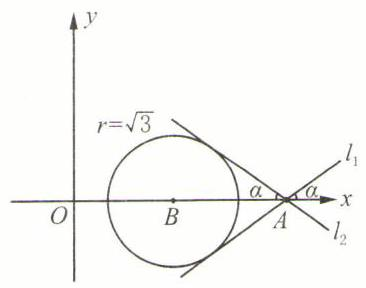
\includegraphics[width=0.3\textwidth]{bodyxb/src/bo_d20cdrf7aajc73bfmvhg_92_1177_276_366_288_0.jpg}
\end{center}


[第 10(2)题]

(3) $\sqrt{13}$ 提示:方法一:将直线 ${l}_{1}$ 的参数方程代入直线 ${l}_{2}$ ,得 $4 + \dfrac{6\sqrt{13}}{13}t + 3 + \dfrac{4\sqrt{13}}{13}t - 2 = 0$ ,解得 $t =  - \dfrac{\sqrt{13}}{2}$ , $\therefore Q\left( {1,1}\right) ,\therefore \left| {PQ}\right|  = \sqrt{{\left( 4 - 1\right) }^{2} + {\left( 3 - 1\right) }^{2}} = \sqrt{13}$ . 方法二: 将直线 ${l}_{1}$ 写成 $\left\{  {\begin{array}{l} x = {x}_{0} + t\cos \alpha , \\  y = {y}_{0} + t\sin \alpha  \end{array}\left( {t\text{ 为参数 }}\right) }\right.$ 的形式,即作变量替换 ${t}^{\prime } = {2t}$ ,则 ${l}_{1} : \left\{  \begin{array}{l} x = 4 + \dfrac{3\sqrt{13}}{13}{t}^{\prime }, \\  y = 3 + \dfrac{2\sqrt{13}}{13}{t}^{\prime } \end{array}\right.$ ( ${t}^{\prime }$ 为参数),代入直线 ${l}_{2}$ 的方程: $4 + \dfrac{3\sqrt{13}}{13}{t}^{\prime } + 3 + \dfrac{2\sqrt{13}}{13}{t}^{\prime } - 2$

$= 0$ ,解得 ${t}^{\prime } =  - \sqrt{13}$ . 根据参数 ${t}^{\prime }$ 的几何意义,易知: $\left| {PQ}\right|  = \left| {t}^{\prime }\right|  = \sqrt{13}$ . 注:对比“方法一”和“方法二”,可以明显看到只有当直线的参数方程满足一定条件时,参数 $t$ 才是有明确几何意义的. 在本题中,根据 “方法一” 得到 $t =$  $- \dfrac{\sqrt{13}}{2}$ ,并进一步推论 $\left| {PQ}\right|  = \left| t\right|  = \dfrac{\sqrt{13}}{2}$ 显然是错误的. 那么,“方法二”中的 ${t}^{\prime } = {2t}$ ,这里的“2”又是怎么来的呢? 对比参数方程 ( $t$ 为参数): $\left\{  \begin{array}{l} x = {x}_{0} + {at}, \\  y = {y}_{0} + {bt} \end{array}\right.$ 和 $\left\{  \begin{array}{l} x = {x}_{0} + t \cdot  \cos \alpha , \\  y = {y}_{0} + t \cdot  \sin \alpha , \end{array}\right.$ 不难发现,作变量替换 $t = \dfrac{{t}^{\prime }}{\sqrt{{a}^{2} + {b}^{2}}}\left( {a \geq  0}\right)$ 或 $t =$  $- \dfrac{{t}^{\prime }}{\sqrt{{a}^{2} + {b}^{2}}}\left( {a < 0}\right)$ 即可. 因此,“方法二”中的“2”,事实上是 $\sqrt{{\left( \dfrac{6\sqrt{13}}{13}\right) }^{2} + {\left( \dfrac{4\sqrt{13}}{13}\right) }^{2}} = 2$ .

(4)-4提示:易知,直线 $l$ 过点(3, - 2)且倾斜角 $\theta$ 满足 $\tan \theta  = \dfrac{3}{4}$ . 设过点 $P\left( {4, - 1}\right)$ 且平行于直线 $l$ 的直线方程为 $y$  $= \dfrac{3}{4}x + b$ ,代入 $P\left( {4, - 1}\right)$ ,得 $- 1 = 3 + b$ , $\therefore \;$ 所求截距为 $b =  - 4$ .

(5) $\left( {\dfrac{11}{5},\dfrac{2}{5}}\right)$ 或 $\left( {-\dfrac{1}{5},\dfrac{18}{5}}\right)$ 提示:方法一:设点 $P\left( {{x}_{P},{y}_{P}}\right)$ ,则 $\sqrt{{\left( {x}_{P} - 1\right) }^{2} + {\left( {y}_{P} - 2\right) }^{2}} = \sqrt{9{t}^{2} + {16}{t}^{2}} = 5\left| t\right|  = 2$ , $\therefore t =  \pm  \dfrac{2}{5}$ . 点 $P$ 的坐标为 $\left( {-\dfrac{1}{5},\dfrac{18}{5}}\right)$ 或 $\left( {\dfrac{11}{5},\dfrac{2}{5}}\right)$ . 方法二: 运用 (3) 中提到的技巧,将直线方程作变量替换 $t =  - \dfrac{1}{5}{t}^{\prime }$ ,得 $\left\{  \begin{array}{l} x = 1 + \dfrac{3}{5}{t}^{\prime }, \\  y = 2 - \dfrac{4}{5}{t}^{\prime } \end{array}\right.$ ( ${t}^{\prime }$ 为参数). 将 ${t}^{\prime } =  \pm  2$ 代入上述方程,即可求得点 $P$ 的坐标,为 $\left( {\dfrac{11}{5},\dfrac{2}{5}}\right)$ 或 $\left( {-\dfrac{1}{5},\dfrac{18}{5}}\right)$ .

11. (1) $2\sqrt{21}$ 提示: 化参数方程为普通方程: ${\left( \dfrac{x - 4}{2}\right) }^{2} + {\left( \dfrac{y - 1}{5}\right) }^{2} = 1$ ,作平移变换: $\left\{  \begin{array}{l} {x}^{\prime } = x - 4, \\  {y}^{\prime } = y - 1, \end{array}\right.$ 得 $\dfrac{{x}^{\prime 2}}{{2}^{2}} + \dfrac{{y}^{\prime 2}}{{5}^{2}} = 1,c =$  $\sqrt{{5}^{2} - {2}^{2}} = \sqrt{21},\therefore$ 焦距为 $2\sqrt{21}$ (焦点在坐标系 ${x}^{\prime }{O}^{\prime }{y}^{\prime }$ 的 ${y}^{\prime }$ 轴上).

(2) $\dfrac{\pi }{3}$ 提示:化参数方程为普通方程: ${\left( \dfrac{y + 2}{3}\right) }^{2} - {\left( \dfrac{x - 1}{\sqrt{3}}\right) }^{2} = 1$ ,作平移变换: $\left\{  \begin{array}{l} {x}^{\prime } = x - 1, \\  {y}^{\prime } = y + 2, \end{array}\right.$ 得 $\dfrac{{y}^{\prime 2}}{{3}^{2}} - \dfrac{{x}^{\prime 2}}{{\left( \sqrt{3}\right) }^{2}} = 1$ ,其渐近线

为 $\dfrac{{y}^{\prime }}{3} \pm  \dfrac{{x}^{\prime }}{\sqrt{3}} = 0$ ,即 ${y}^{\prime } =  \pm  \sqrt{3}{x}^{\prime }$ ,渐近线的倾斜角分别为 $\arctan \left( \sqrt{3}\right)  = \dfrac{\pi }{3}$ 和 $\pi  + \arctan \left( {-\sqrt{3}}\right)  = \dfrac{2\pi }{3},\therefore$ 渐近线的夹角为 $\dfrac{2\pi }{3} - \dfrac{\pi }{3} = \dfrac{\pi }{3}$ .

(3) $\left( {1 - \sqrt{7},0}\right)$ 提示: 化参数方程为普通方程: ${\left( \dfrac{x - 1}{4}\right) }^{2} + {\left( \dfrac{y}{3}\right) }^{2} = 1$ ,作平移变换: $\left\{  \begin{array}{l} {x}^{\prime } = x - 1, \\  {y}^{\prime } = y, \end{array}\right.$ 得 $\dfrac{{x}^{\prime 2}}{{4}^{2}} + \dfrac{{y}^{\prime 2}}{{3}^{2}} = 1,c =$  $\sqrt{{4}^{2} - {3}^{2}} = \sqrt{7}$ ,在坐标系 ${x}^{\prime }{O}^{\prime }{y}^{\prime }$ 中,椭圆的左焦点为 $\left( {-\sqrt{7},0}\right)$ . 在坐标系 ${xOy}$ 中,椭圆的左焦点为 $\left( {1 - \sqrt{7},0}\right)$ .

(4) $y = \dfrac{1}{2}$ 提示: 化参数方程为普通方程: $y = 2 \cdot  {\left( \dfrac{x}{2}\right) }^{2} + 1$ ,即 ${x}^{2} = 2\left( {y - 1}\right)$ ,作平移变换: $\left\{  \begin{array}{l} {x}^{\prime } = x, \\  {y}^{\prime } = y - 1, \end{array}\right.$ 得 ${x}^{\prime 2} = 2{y}^{\prime }$ , ${2p} = 2$ ,故 $p = 1$ . 在坐标系 ${x}^{\prime }{O}^{\prime }{y}^{\prime }$ 中,准线方程为 ${y}^{\prime } =  - \dfrac{p}{2} =  - \dfrac{1}{2},\therefore$ 在坐标系 ${xOy}$ 中,准线方程为 $y = 1 - \dfrac{1}{2}$  $= \dfrac{1}{2}$ .

12. (1) 设点 $E,F$ 的坐标分别为 $E\left( {{t}_{1},{t}_{1}^{2}}\right)$ 和 $F\left( {{t}_{2},{t}_{2}^{2}}\right) ,{t}_{1} \neq  {t}_{2}$ ,线段 ${EF}$ 的中点 $P$ 满足参数方程: $\left\{  \begin{array}{l} {x}_{P} = \dfrac{{t}_{1} + {t}_{2}}{2}, \\  {y}_{P} = \dfrac{{t}_{1}^{2} + {t}_{2}^{2}}{2}, \end{array}\right.$

$\therefore {y}_{P} = \dfrac{1}{2}\left\lbrack  {{\left( {t}_{1} + {t}_{2}\right) }^{2} - 2{t}_{1}{t}_{2}}\right\rbrack   = 2{x}_{P}^{2} - {t}_{1}{t}_{2}$ . 下一步,我们寻找 ${t}_{1}{t}_{2}$ 与 ${x}_{P}$ 之间的关系. 不难发现,联立过点 $A$ (2,0)的直线方程和抛物线方程 $y = {x}^{2}$ ,可知 ${t}_{1}{t}_{2}$ 是两根之积. 由于过点 $A$ 且垂直于 $x$ 轴的直线 $\left( {x = 2}\right)$ 与抛物线仅有一个交点,不合题意,因此,过点 $A$ 的直线方程可设为 $y = k\left( {x - 2}\right)$ . 联立 $\left\{  \begin{array}{l} y = k\left( {x - 2}\right) , \\  y = {x}^{2}, \end{array}\right.$ 得 ${x}^{2} - {kx} + {2k} = 0$ ,

$\therefore \;{t}_{1} + {t}_{2} = k,{t}_{1}{t}_{2} = {2k},\;\therefore \;{t}_{1}{t}_{2} = 2\left( {{t}_{1} + {t}_{2}}\right)  = 4{x}_{P},\;\therefore \;{y}_{P} = 2{x}_{P}^{2} - 4{x}_{P}.\;\therefore \;$ 点 $P$ 的轨迹方程为 $y = 2{x}^{2}$  $- {4x}$ (在原抛物线内的部分) (即 $x < 0$ 或 $x > 4$ ).

(2)由题意,设这两个锐角为 $\theta$ 和 $\dfrac{\pi }{2} - \theta$ . $\;\therefore \left\{  \begin{array}{l} \sin \theta  + \sin \left( {\dfrac{\pi }{2} - \theta }\right)  = a, \\  \sin \theta  \cdot  \sin \left( {\dfrac{\pi }{2} - \theta }\right)  = b, \end{array}\right.$ 即 $\left\{  {\begin{array}{l} a = \sin \theta  + \cos \theta , \\  b = \sin \theta  \cdot  \cos \theta . \end{array}{a}^{2} = 1 + 2\sin \theta \cos \theta  = 1 + {2b}}\right.$ . $\because \theta  \in  \left( {0,\dfrac{\pi }{2}}\right) ,\;\therefore a = \sqrt{2}\sin \left( {\theta  + \dfrac{\pi }{4}}\right)  \in  \left( {1,\sqrt{2}}\right\rbrack  .\;\therefore$ 点(a, b)轨迹的普通方程为 ${x}^{2} = 1 + {2y}\left( {1 < x \leq  \sqrt{2}}\right)$ .

(3) 联立 $\left\{  \begin{array}{l} y = \dfrac{1}{4}{x}^{2}, \\  {tx} - {2y} + {2t} = 0, \end{array}\right.$ 得 ${x}^{2} - {2tx} - {4t} = 0,{x}_{1} + {x}_{2} = {2t},{x}_{1}{x}_{2} =  - {4t}$ . 所求中点轨迹的参数方程为 $\left\{  {\begin{array}{l} x = \dfrac{{x}_{1} + {x}_{2}}{2} = t, \\  y = \dfrac{{y}_{1} + {y}_{2}}{2} = \dfrac{1}{8}\left( {{x}_{1}^{2} + {x}_{2}^{2}}\right) . \end{array}\therefore \;y = \dfrac{1}{8}\left\lbrack  {{\left( {x}_{1} + {x}_{2}\right) }^{2} - 2{x}_{1}{x}_{2}}\right\rbrack   = \dfrac{1}{8}\left( {4{t}^{2} + {8t}}\right)  = \dfrac{1}{2}{t}^{2} + t,}\right.$

$\therefore y = \dfrac{1}{2}{x}^{2} + x$ . $\therefore$ 所求中点的轨迹方程为 $y = \dfrac{1}{2}{x}^{2} + x$ (在已知抛物线内的部分) (即 $x > 0$ 或 $x <  - 4$ ).

13. $B$ 提示: 方法一: 将参数方程代入圆的方程: ${\left( 1 + 2t\right) }^{2} + {\left( 2 + t\right) }^{2} = 9$ ,整理得 $5{t}^{2} + {8t} - 4 = 0,\therefore {t}_{1} = \dfrac{2}{5},{t}_{2} =  - 2$ .

$\therefore$ 弦的两个端点坐标为 $\left( {\dfrac{9}{5},\dfrac{12}{5}}\right)$ 和(-3,0). $\therefore$ 弦长为 $\sqrt{{\left( -3 - \dfrac{9}{5}\right) }^{2} + {\left( 0 - \dfrac{12}{5}\right) }^{2}} = \dfrac{12}{5}\sqrt{5}$ . 方法二:运用第 ${10}\left( 3\right)$ 题提到的技巧,将直线方程作变量替换 $t = \dfrac{{t}^{\prime }}{\sqrt{5}}$ ,得 $\left\{  \begin{array}{l} x = 1 + \dfrac{2}{\sqrt{5}}{t}^{\prime } \\  y = 2 + \dfrac{1}{\sqrt{5}}{t}^{\prime } \end{array}\right.$ ( ${t}^{\prime }$ 为参数). 代入 ${x}^{2} + {y}^{2} = 9$ ,整理得 ${t}^{\prime 2} + \dfrac{8}{\sqrt{5}}{t}^{\prime } - 4 = 0$ ,弦长即 $\left| {{t}_{1}^{\prime } - {t}_{2}^{\prime }}\right|  = \sqrt{{\left( {t}_{1}^{\prime } + {t}_{2}^{\prime }\right) }^{2} - 4{t}_{1}^{\prime } \cdot  {t}_{2}^{\prime }} = \sqrt{{\left( -\dfrac{8}{\sqrt{5}}\right) }^{2} - 4 \cdot  \left( {-4}\right) } = \dfrac{12}{5}\sqrt{5}$ . 方法三:设直线与圆交于 $\left( {{x}_{1},{y}_{1}}\right) ,\left( {{x}_{2},{y}_{2}}\right)$ 两

点,对应参数分别为 ${t}_{1},{t}_{2}$ ,则弦长为 $\sqrt{{\left( {x}_{2} - {x}_{1}\right) }^{2} + {\left( {y}_{2} - {y}_{1}\right) }^{2}} = \sqrt{4{\left( {t}_{2} - {t}_{1}\right) }^{2} + {\left( {t}_{2} - {t}_{1}\right) }^{2}} = \sqrt{5} \cdot  \left| {{t}_{2} - {t}_{1}}\right|$ . 欲求 $\left| {{t}_{2} - {t}_{1}}\right|$ ,需将参数方程代入圆的方程: ${\left( 1 + 2t\right) }^{2} + {\left( 2 + t\right) }^{2} = 9$ ,整理得 $5{t}^{2} + {8t} - 4 = 0.\;\therefore \;\sqrt{5} \cdot  \left| {{t}_{2} - {t}_{1}}\right|  =$  $\sqrt{5} \times  \sqrt{{\left( {t}_{1} + {t}_{2}\right) }^{2} - 4{t}_{1}{t}_{2}} = \sqrt{5} \times  \sqrt{{\left( -\dfrac{8}{5}\right) }^{2} - 4 \cdot  \left( {-\dfrac{4}{5}}\right) } = \dfrac{12}{5}\sqrt{5}$ . 注:“方法一”仅当交点坐标容易求得具体值时,才比较

方便,否则计算量会很大；“方法二”和“方法三”都涉及韦达定理的使用,一般能简化计算. 其中,“方法二”还用到了直线参数方程的参数含义. 本章后续解题过程将尽可能采用简便的方法.

14. A 提示: 设 ${M}_{1}\left( {{x}_{1},{y}_{1}}\right) ,{M}_{2}\left( {{x}_{2},{y}_{2}}\right) \left( {{x}_{1} \neq  {x}_{2}}\right) .\;\because {x}_{1} \neq  {x}_{2},\;\therefore {t}_{1} \neq  {t}_{2},\;\therefore$ 弦 ${M}_{1}{M}_{2}$ 所在直线的斜率为 $\dfrac{{y}_{2} - {y}_{1}}{{x}_{2} - {x}_{1}} = \dfrac{{2p}\left( {{t}_{2}^{2} - {t}_{1}^{2}}\right) }{{2p}\left( {{t}_{2} - {t}_{1}}\right) } = {t}_{1} + {t}_{2}.$

15. C 提示: 作变量替换 $t =  - \dfrac{1}{2}{t}^{\prime }$ ,得 $\left\{  \begin{array}{l} x =  - 2 + \dfrac{\sqrt{2}}{2}{t}^{\prime }, \\  y = 3 - \dfrac{\sqrt{2}}{2}{t}^{\prime } \end{array}\right.$ ( ${t}^{\prime }$ 为参数),是经过点 $P\left( {-2,3}\right)$ ,斜率为-1的直线. 与点 $P$ 的距离为 $\sqrt{2}$ 的点为 $\left( {-2 \pm  \dfrac{\sqrt{2}}{2} \cdot  \sqrt{2},3 \mp  \dfrac{\sqrt{2}}{2} \cdot  \sqrt{2}}\right)$ ,即(-1,2)或(-3,4).

16. A 提示: 作变量替换 $t = \dfrac{1}{2}{t}^{\prime }$ ,得 $\left\{  \begin{array}{l} x = 2 + \dfrac{1}{2}{t}^{\prime }, \\  y = \dfrac{\sqrt{3}}{2}{t}^{\prime }\left( {{t}^{\prime }\text{ 为参数 }}\right) . \end{array}\right.$ 代入双曲线 ${x}^{2} - {y}^{2} = 1$ ,整理得: ${t}^{\prime 2} - 4{t}^{\prime } - 6 = 0$ ,弦长即 $\left| {{t}^{\prime }{}_{2} - {t}^{\prime }{}_{1}}\right|  = \sqrt{{\left( {t}^{\prime }{}_{1} + {t}^{\prime }{}_{2}\right) }^{2} - 4{t}^{\prime }{}_{1}{t}^{\prime }{}_{2}} = \sqrt{{4}^{2} - 4 \cdot  \left( {-6}\right) } = 2\sqrt{10}.$

17. $C$ 提示: 由题意, $\left| {z \mp  \sqrt{2}a\mathrm{i}}\right|$ 的几何含义是点(x, y)到点 $\left( {0, \pm  \sqrt{2}a}\right)$ 的距离.

$\therefore \left| {z - \sqrt{2}a\mathrm{i}}\right|  - \left| {z + \sqrt{2}a\mathrm{i}}\right|  = {2a}\left( {a > 0}\right)$ 代表焦点为 $\left( {0, \pm  \sqrt{2}a}\right)$ ,且实轴长为 ${2a}$ 的双曲线的下支. 又 $b = \sqrt{{c}^{2} - {a}^{2}} =$  $\sqrt{{\left( \sqrt{2}a\right) }^{2} - {a}^{2}} = a,\therefore \left( {x,y}\right)$ 代表双曲线 $\dfrac{{y}^{2}}{{a}^{2}} - \dfrac{{x}^{2}}{{a}^{2}} = 1$ 的下支 $\left( {y < 0}\right)$ 上的点. 写成参数方程即 $\left\{  \begin{array}{l} x = a \cdot  \tan \theta , \\  y = \dfrac{a}{\cos \theta } \end{array}\right.$ ( $\theta$ 为参数),其中 $y = \dfrac{a}{\cos \theta } < 0$ ,且 $0 \leq  \theta  < {2\pi },\;\therefore \;\theta  \in  \left( {\dfrac{\pi }{2},\dfrac{3\pi }{2}}\right)$ .

18. (1) ${x}^{2} - {y}^{2} = 4\left( {x \geq  2}\right)$ 提示: ${x}^{2} = {\mathrm{e}}^{2t} + {\mathrm{e}}^{-{2t}} + 2,{y}^{2} = {\mathrm{e}}^{2t} + {\mathrm{e}}^{-{2t}} - 2,\therefore {x}^{2} - {y}^{2} = 4,t \in  \mathbf{R}$ 时, $x = {\mathrm{e}}^{t} + {\mathrm{e}}^{-t} \geq  2$ ,

$\therefore$ 原参数方程的普通方程为 ${x}^{2} - {y}^{2} = 4\left( {x \geq  2}\right)$ .

(2) ${x}^{2} + {y}^{2} = 1\left( {x \neq   - 1}\right)$ 提示: 令 $t = \tan \dfrac{\alpha }{2},\alpha  \in  \left( {-\pi ,\pi }\right) ,\;\therefore \left\{  {\begin{array}{l} x = \dfrac{1 - {t}^{2}}{1 + {t}^{2}} = \cos \alpha , \\  y = \dfrac{2t}{1 + {t}^{2}} = \sin \alpha , \end{array}\;\therefore {x}^{2} + {y}^{2} = 1}\right.$ .

$\because \alpha  \in  \left( {-\pi ,\pi }\right) ,\;\therefore x \in  ( - 1,1\rbrack ,y \in  \left\lbrack  {-1,1}\right\rbrack  .\;\therefore$ 原参数方程的普通方程为 ${x}^{2} + {y}^{2} = 1\left( {x \neq   - 1}\right)$ .

(3) ${y}^{2} =  - 2\left( {x - \dfrac{1}{2}}\right)$ 提示: $x = 1 - \dfrac{1}{1 + \cos \theta },\;\therefore \dfrac{1}{1 + \cos \theta } = 1 - x$ . 又 ${x}^{2} + {y}^{2} = \dfrac{{\cos }^{2}\theta  + {\sin }^{2}\theta }{{\left( 1 + \cos \theta \right) }^{2}} = \dfrac{1}{{\left( 1 + \cos \theta \right) }^{2}} = (1 -$  $x{)}^{2}$ ,整理得 ${y}^{2} =  - {2x} + 1 =  - 2\left( {x - \dfrac{1}{2}}\right) {.1} + \cos \theta  \neq  0$ ,故 $\cos \theta  \neq   - 1$ ,即 $\cos \theta  \in  ( - 1,1\rbrack$ , $\therefore x \leq  \dfrac{1}{2}.\;\therefore$ 原参数方程的普通方程为 ${y}^{2} =  - 2\left( {x - \dfrac{1}{2}}\right)$ .

(4) $\dfrac{{x}^{2}}{4} + {y}^{2} = 1\left( {y \neq   - 1}\right)$ 提示:方法一: $\left\{  {\begin{array}{l} x = \dfrac{8t}{4 + {t}^{2}}, \\  y =  - 1 + \dfrac{8}{4 + {t}^{2}}, \end{array}\;\therefore \;\left( {y + 1}\right)  \cdot  t = x}\right.$ . 显然, $y + 1 \neq  0,\;\therefore \;t = \dfrac{x}{y + 1}$ ,代入 $x = \dfrac{8t}{4 + {t}^{2}}$ ,得 $x = \dfrac{8 \cdot  \dfrac{x}{y + 1}}{4 + {\left( \dfrac{x}{y + 1}\right) }^{2}} = \dfrac{{8x}\left( {y + 1}\right) }{4{\left( y + 1\right) }^{2} + {x}^{2}}$ ,整理得 $x\left\lbrack  {4\left( {{y}^{2} - 1}\right)  + {x}^{2}}\right\rbrack   = 0,x \neq  0$ 时, $t \neq  0,\dfrac{{x}^{2}}{4} + {y}^{2} = 1(x \neq  0,y$  $\neq   \pm  1)$ ,又注意到 $x = 0$ 时, $t = 0,y = 1$ . 点(0,1)也在曲线 $\dfrac{{x}^{2}}{4} + {y}^{2} = 1$ 上, $\therefore$ 只有点(0, - 1)不在原参数方程上,

$\therefore$ 原参数方程的普通方程为 $\dfrac{{x}^{2}}{4} + {y}^{2} = 1\left( {y \neq   - 1}\right)$ .

方法二: 令 $t = 2{t}^{\prime }\left( {{t}^{\prime } \in  \mathbf{R}}\right)$ ,

$\therefore \left\{  \begin{array}{l} x = \dfrac{{16}{t}^{\prime }}{4 + 4{t}^{\prime 2}} = \dfrac{4{t}^{\prime }}{1 + {t}^{\prime 2}}, \\  y = \dfrac{4 - 4{t}^{\prime 2}}{4 + 4{t}^{\prime 2}} = \dfrac{1 - {t}^{\prime 2}}{1 + {t}^{\prime 2}}. \end{array}\right.$ 再令 ${t}^{\prime } = \tan \dfrac{\alpha }{2}$ ,利用万能公式,得 $\left\{  \begin{array}{l} x = 2\sin \alpha , \\  y = \cos \alpha , \end{array}\right.$

$\therefore \dfrac{{x}^{2}}{4} + {y}^{2} = 1.\;\because \alpha  \in  \left( {-\pi ,\pi }\right) ,\;\therefore x \in  \left\lbrack  {-1,1}\right\rbrack  ,y \in  ( - 1,1\rbrack$ ,

$\therefore$ 原参数方程的普通方程为 $\dfrac{{x}^{2}}{4} + {y}^{2} = 1\left( {y \neq   - 1}\right)$ .

19. (1) $\left\{  \begin{array}{l} x = 2{\cos }^{2}\theta , \\  y = \sin {2\theta } \end{array}\right.$ ( $\theta$ 为参数, $0 \leq  \theta  < \pi$ ) 提示:方法一:过原点、倾斜角为 $\theta$ 的直线方程为 $l : y = x \cdot  \tan \theta ,(\theta  \in  \lbrack 0,\pi )$ 且 $\theta$  $\left. { \neq  \dfrac{\pi }{2}}\right)$ 或 $l : x = 0\left( {\theta  = \dfrac{\pi }{2}}\right)$ . 先看 $\theta  \neq  \dfrac{\pi }{2}$ 的情况: 将 $y = x \cdot  \tan \theta$ 代入圆的方程中,得 ${x}^{2} + {x}^{2} \cdot  {\tan }^{2}\theta  - {2x} = 0$ ,

$\therefore \dfrac{{x}^{2}}{{\cos }^{2}\theta } - {2x} = 0.\;\therefore x \neq  0$ 时, $x = 2{\cos }^{2}\theta .y = x \cdot  \tan \theta  = 2\sin \theta \cos \theta  = \sin {2\theta }$ . 而 $\theta  = \dfrac{\pi }{2}$ 时, $2{\cos }^{2}\theta  = 0,\sin {2\theta } = 0$ ,此时直线 $l$ 与圆相切于原点 $O$ ,也能用 $\left( {x,y}\right)  = \left( {2{\cos }^{2}\theta ,\sin {2\theta }}\right)$ 表示. 综上,圆用 $\theta$ 表示的参数方程为 $\left\{  \begin{array}{l} x = 2{\cos }^{2}\theta , \\  y = \sin {2\theta } \end{array}\right.$ ( $\theta$ 为参数, $0 \leq  \theta  < \pi$ ). 方法二: 将直线记为 $l$ ,圆 ${x}^{2} + {y}^{2} - {2x} = 0$ 记为 $\odot  C : {\left( x - 1\right) }^{2} + {y}^{2} = 1$ ,是以 $C\left( {1,0}\right)$ 为圆心,半径为 1 的圆. 直线 $l$ 与圆 $C$ 交于原点 $O$ 和另一点 (如有,记为点 $A$ ). ①当 $0 < \theta  < \dfrac{\pi }{2}$ 时,解 $\bigtriangleup  {OCA},\because \left| {CO}\right|  = \left| {CA}\right|  =$  $1,\angle {COA} = \angle {CAO} = \theta ,\therefore \angle {OCA} = \pi  - {2\theta }$ . 利用正弦定理: $\dfrac{\left| OA\right| }{\sin \angle {OCA}} = \dfrac{\left| OC\right| }{\sin \angle {CAO}},\therefore \left| {OA}\right|  = \dfrac{\left| OC\right| }{\sin \theta }$ . $\sin \left( {\pi  - {2\theta }}\right)  = 2\cos \theta ,\;\therefore \;{x}_{A} = \left| {OA}\right|  \cdot  \cos \theta  = 2{\cos }^{2}\theta ,{y}_{A} = \left| {OA}\right|  \cdot  \sin \theta  = \sin {2\theta }$ . ② 当 $\dfrac{\pi }{2} < \theta  < \pi$ 时,类似地, $\angle {COA} = \angle {CAO} = \pi  - \theta ,$

$\therefore \angle {OCA} = \pi  - 2\left( {\pi  - \theta }\right)  = {2\theta } - \pi$ . 由正弦定理: $\dfrac{\left| OA\right| }{\sin \angle {OCA}} = \dfrac{\left| OC\right| }{\sin \angle {CAO}},\left| {OA}\right|  = \dfrac{\left| OC\right| }{\sin \left( {\pi  - \theta }\right) } \cdot  \sin \left( {{2\theta } - \pi }\right)  =$  $- 2\cos \theta ,\therefore {x}_{A} = \left| {OA}\right|  \cdot  \cos \left( {\pi  - \theta }\right)  = 2{\cos }^{2}\theta ,{y}_{A} =  - \left| {OA}\right|  \cdot  \sin \left( {\pi  - \theta }\right)  = \sin {2\theta }$ . ③当 $\theta  = 0$ 时,交点为 $A(2$ , $0)$ ; 当 $\theta  = \dfrac{\pi }{2}$ 时,交点为 $A\left( {0,0}\right)$ ,均能写成 $\left( {x,y}\right)  = \left( {2{\cos }^{2}\theta ,\sin {2\theta }}\right)$ 的形式. 综上,圆用 $\theta$ 表示的参数方程为: $\left\{  {\begin{array}{l} x = 2{\cos }^{2}\theta , \\  y = \sin {2\theta } \end{array}\left( {\theta \text{ 为参数, }0 \leq  \theta  < \pi }\right) .}\right.$

(2) $\left\{  \begin{array}{l} x =  - \dfrac{8t}{4 + {t}^{2}}\text{ ( }t\text{ 为参数) } \\  y = \dfrac{{16} - 4{t}^{2}}{4 + {t}^{2}}\text{ ( }t\text{ 为参数) } \end{array}\right.$ 即点(0, - 4)提示: 点 $A\left( {0,4}\right)$ 在椭圆 $4{x}^{2} + {y}^{2} = {16}$ 上,直线方程可写为 $y - 4 = {tx}(t \in$

R),代入 $4{x}^{2} + {y}^{2} = {16}$ ,整理得 ${x}^{2}\left( {{t}^{2} + 4}\right)  + {8tx} = 0.\;\therefore$ 当 $x \neq  0$ ,即 $t \neq  0$ 时, $x =  - \dfrac{8t}{4 + {t}^{2}},y = {tx} + 4 = \dfrac{{16} - 4{t}^{2}}{4 + {t}^{2}}$ . $t = 0$ 时, $x = 0,y = 4,t \in  \mathbf{R}$ 时, $x \in  \left\lbrack  {-2,2}\right\rbrack$ ,而 $y =  - 4 + \dfrac{32}{4 + {t}^{2}},y \in  ( - 4,4\rbrack$ . 故参数方程不包括点(0, - 4)(垂直于 $x$ 轴的直线斜率不存在), $\;\therefore$ 椭圆的参数方程为 $\left\{  \begin{array}{l} x =  - \dfrac{8t}{4 + {t}^{2}}, \\  y = \dfrac{{16} - 4{t}^{2}}{4 + {t}^{2}} \end{array}\right.$ ( $t$ 为参数)和点(0, - 4).

20. (1) 将直线的参数方程代入圆,得 ${\left( 1 + \dfrac{1}{2}t\right) }^{2} + {\left( -3\sqrt{3} + \dfrac{\sqrt{3}}{2}t\right) }^{2} = {16}$ ,整理得 ${t}^{2} - {8t} + {12} = 0,\;\therefore \;{t}_{1} = 6,{t}_{2} = 2$ . 对应地 $\left( {{x}_{1},{y}_{1}}\right)  = \left( {4,0}\right) ,\left( {{x}_{2},{y}_{2}}\right)  = \left( {2, - 2\sqrt{3}}\right) ,{AB}$ 的中点为 $\left( {\dfrac{{x}_{1} + {x}_{2}}{2},\dfrac{{y}_{1} + {y}_{2}}{2}}\right)  = \left( {3, - \sqrt{3}}\right)$ .

(2)作变量替换: $t = \dfrac{1}{2}{t}^{\prime }$ ,得 $\left\{  \begin{array}{l} x = 1 + \dfrac{1}{2}{t}^{\prime }, \\  y = 5 + \dfrac{\sqrt{3}}{2}{t}^{\prime }, \end{array}\right.$ 代入 ${x}^{2} + {y}^{2} = {16}$ ,整理得 ${t}^{\prime 2} + \left( {5\sqrt{3} + 1}\right) {t}^{\prime } + {10} = 0,\Delta  > 0,{t}_{1}^{\prime } + {t}_{2}^{\prime } =  - (5\sqrt{3} +$  $1),{t}_{1}^{\prime } \cdot  {t}_{2}^{\prime } = {10}$ ,可见 ${t}_{1}^{\prime },{t}_{2}^{\prime }$ 同号,且 ${t}_{1}^{\prime } < 0,{t}_{2}^{\prime } < 0$ , $\therefore \left| {PA}\right|  + \left| {PB}\right|  = \left| {t}_{1}^{\prime }\right|  + \left| {t}_{2}^{\prime }\right|  =  - \left( {{t}_{1}^{\prime } + {t}_{2}^{\prime }}\right)  = 5\sqrt{3} + 1$ .

(3) 设直线的参数方程为 $l : \left\{  \begin{array}{l} x = 1 + t \cdot  \cos \alpha , \\  y =  - 2 + t \cdot  \sin \alpha  \end{array}\right.$ ( $t$ 为参数) $\left( {\alpha  \in  \lbrack 0,\pi }\right)$ ). 将 $l$ 代入 ${x}^{2} + 2{y}^{2} = 8$ ,整理得 $\left( {1 + {\sin }^{2}\alpha }\right) {t}^{2} +$  $\left( {2\cos \alpha  - 8\sin \alpha }\right) t + 1 = 0\left( *\right) ,\left| {PA}\right|  \cdot  \left| {PB}\right|  = \left| {t}_{1}\right|  \cdot  \left| {t}_{2}\right|  = \dfrac{1}{1 + {\sin }^{2}\alpha } = \dfrac{2}{3},\;\therefore \;{\sin }^{2}\alpha  = \dfrac{1}{2},\;\therefore \;\alpha  = \dfrac{\pi }{4}$ 或 $\dfrac{3\pi }{4}$ [均能使方程 ( $x$ ) 的 $\Delta  > 0\rbrack$ .

21. (1) 方法一: 将 $\left\{  \begin{array}{l} x = 2 + \dfrac{t}{2} \\  y = \dfrac{\sqrt{3}}{2}t \end{array}\right.$ ,代入 ${x}^{2} - {y}^{2} = 1$ ,整理得 ${t}^{2} - {4t} - 6 = 0,\therefore {t}_{1} + {t}_{2} = 4,{t}_{1} \cdot  {t}_{2} =  - 6$ ,所求弦长 $=$  $\sqrt{{\left( {x}_{2} - {x}_{1}\right) }^{2} + {\left( {y}_{2} - {y}_{1}\right) }^{2}} = \sqrt{\dfrac{1}{4}{\left( {t}_{2} - {t}_{1}\right) }^{2} + \dfrac{3}{4}{\left( {t}_{2} - {t}_{1}\right) }^{2}} = \sqrt{{\left( {t}_{1} + {t}_{2}\right) }^{2} - 4{t}_{1} \cdot  {t}_{2}} = 2\sqrt{10}.$

方法二:注意到,直线的参数方程的 $t$ 的几何含义是明确的,即: $\left| t\right|$ 表示点(x, y)到点(2,0)的距离. 因此,将直线的参数方程代入 ${x}^{2} - {y}^{2} = 1$ ,得到 ${t}^{2} - {4t} - 6 = 0$ 后,由 ${t}_{1} + {t}_{2} = 4,{t}_{1} \cdot  {t}_{2} =  - 6$ 可知弦长 $= \left| {{t}_{1} - {t}_{2}}\right|  =$  $\sqrt{{\left( {t}_{1} + {t}_{2}\right) }^{2} - 4{t}_{1} \cdot  {t}_{2}} = 2\sqrt{10}.$

(2)不难看出,曲线是以点(2,1)为顶点的抛物线,故设直线 $l : \left\{  {\begin{array}{l} x = 2 + s \cdot  \cos \alpha , \\  y = 1 + s \cdot  \sin \alpha  \end{array}\left( {s\text{ 是参数, }\alpha  \in  \lbrack 0,\pi ))}\right. }\right.$ ,代入曲线 $\left\{  \begin{array}{l} x = 2 + 2{t}^{2}, \\  y = 1 - \sqrt{3}t, \end{array}\right.$ 得 $s \cdot  \cos \alpha  = 2{t}^{2},s \cdot  \sin \alpha  =  - \sqrt{3}t$ ,消去参数 $t$ ,得 ${s}^{2}{\sin }^{2}\alpha  - \dfrac{3}{2}s \cdot  \cos \alpha  = 0,\alpha  \neq  0$ ,否则 $l$ 与曲线仅有一个交点. $\therefore {s}_{1} + {s}_{2} = \dfrac{3\cos \alpha }{2{\sin }^{2}\alpha },{s}_{1} \cdot  {s}_{2} = 0$ ,弦长 $= \left| {{s}_{1} - {s}_{2}}\right|  = \sqrt{{\left( {s}_{1} + {s}_{2}\right) }^{2} - 4{s}_{1}{s}_{2}} = \dfrac{3\left| {\cos \alpha }\right| }{2{\sin }^{2}\alpha } = 1$ ,

$\therefore 2{\cos }^{2}\alpha  + 3\left| {\cos \alpha }\right|  - 2 = 0,\left| {\cos \alpha }\right|  = \dfrac{1}{2}$ 或 $\left| {\cos \alpha }\right|  =  - 2$ (舍去), $\;\therefore \;\alpha  = \dfrac{\pi }{3}$ 或 $\dfrac{2\pi }{3}$ .

(3) ${2p} = 4,p = 2$ ,故 ${y}^{2} = {4x}$ 的焦点为 $F\left( {1,0}\right)$ . 设直线 ${AB}$ 的参数方程为: $\left\{  \begin{array}{l} x = 1 + t \cdot  \cos \alpha , \\  y = t \cdot  \sin \alpha  \end{array}\right.$ ( $t$ 为参数),其中 $\alpha  \in  \left( {0,\pi }\right)$  $\left( {\alpha  = 0\text{ 时,直线与抛物线仅一个交点,不合题意). 代入 }{y}^{2} = {4x}\text{ ,整理得 }{t}^{2}{\sin }^{2}\alpha  - {4t}\cos \alpha  - 4 = 0\text{ , }}\right)$

$\therefore \left\{  {\begin{array}{l} {t}_{1} + {t}_{2} = \dfrac{4\cos \alpha }{{\sin }^{2}\alpha }, \\  {t}_{1} \cdot  {t}_{2} =  - \dfrac{4}{{\sin }^{2}\alpha } < 0 \end{array}\left( *\right) }\right.$ . 其中 ${t}_{1},{t}_{2}$ 分别是 $A,B$ 对应的参数,

$\therefore \left| {FA}\right|  : \left| {FB}\right|  = 1 : 2 = \left| {t}_{1}\right|  : \left| {t}_{2}\right|  =  - \dfrac{{t}_{1}}{{t}_{2}}$ . 将 ${t}_{2} =  - 2{t}_{1}$ 代入 (*),消去 ${t}_{1}$ ,得 ${\tan }^{2}\alpha  = 8$ ,

$\therefore$ 斜率 $\tan \alpha  =  \pm  2\sqrt{2}$ ,对应直线方程: $y =  \pm  2\sqrt{2}\left( {x - 1}\right)$ ,即 ${4x} \pm  \sqrt{2}y - 4 = 0$ .

22. (1) 将直线 ${PQ}$ 写为参数方程的形式: $\left\{  \begin{array}{l} x =  - 2 + \dfrac{t}{\sqrt{2}}, \\  y = 4 - \dfrac{t}{\sqrt{2}}, \end{array}\right.$ 代入 ${y}^{2} = {2px}\left( {p > 0}\right)$ ,

整理得 ${t}^{2} - \sqrt{2}\left( {8 + {2p}}\right)  \cdot  t + \left( {{32} + {8p}}\right)  = 0\left( *\right)$ ,

$\therefore \left\{  {\begin{array}{l} {t}_{1} + {t}_{2} = \sqrt{2}\left( {8 + {2p}}\right)  > 0, \\  {t}_{1} \cdot  {t}_{2} = {32} + {8p} > 0 \end{array}\left( {* * }\right) \text{ . 不妨设 }{t}_{1} < {t}_{2},\;\therefore \;\left| {MP}\right|  = {t}_{1},\left| {PQ}\right|  = {t}_{2} - {t}_{1},\left| {MQ}\right|  = {t}_{2}}\right.$ . 由题意有

${\left| PQ\right| }^{2} = \left| {MP}\right|  \cdot  \left| {MQ}\right| ,\therefore {t}_{1}^{2} + {t}_{2}^{2} - 3{t}_{1} \cdot  {t}_{2} = 0$ ,即 ${\left( {t}_{1} + {t}_{2}\right) }^{2} - 5{t}_{1} \cdot  {t}_{2} = 0$ ,代入 $\left( {* * }\right)$ ,得 $p = 1$ . 不难验证, $p = 1$ 时方程 (*) 的 $\Delta  > 0.\;\therefore \;$ 综上, $p = 1$ .

(2)将直线 ${AB}$ 写成参数方程的形式: $\left\{  \begin{array}{l} x = {x}_{P} + \dfrac{t}{\sqrt{2}}, \\  y = {y}_{P} + \dfrac{t}{\sqrt{2}} \end{array}\right.$ ( $t$ 为参数),代入 ${x}^{2} + 2{y}^{2} + {4y} - 1 = 0$ ,整理得 $\dfrac{3}{2}{t}^{2} + \left( {\sqrt{2}{x}_{P} + }\right.$  $2\sqrt{2}{y}_{P} + 2\sqrt{2})t + \left( {{x}_{P}^{2} + 2{y}_{P}^{2} + 4{y}_{P} - 1}\right)  = 0\left( *\right) .\left| {PA}\right|  \cdot  \left| {PB}\right|  = \left| {t}_{1}\right|  \cdot  \left| {t}_{2}\right|  = \left| \dfrac{{x}_{P}^{2} + 2{y}_{P}^{2} + 4{y}_{P} - 1}{\dfrac{3}{2}}\right|  = 2,$

$\therefore \;\left| {{x}_{P}^{2} + 2{y}_{P}^{2} + 4{y}_{P} - 1}\right|  = 3$ .

①当 ${x}_{P}^{2} + 2{y}_{P}^{2} + 4{y}_{P} - 1 =  - 3$ 时, ${x}_{P}^{2} + 2{\left( {y}_{P} + 1\right) }^{2} = 0,\;\therefore \;\left( {{x}_{P},{y}_{P}}\right)  = \left( {0, - 1}\right)$ . 此时 $t =  \pm  \sqrt{2},m =  - 1,y = x - 1$ 与曲线交于点(1,0)和(-1, - 2).

②当 ${x}_{P}^{2} + 2{y}_{P}^{2} + 4{y}_{P} - 1 = 3$ 时,这本身就是关于点 $P$ 的轨迹方程,接下来确定该轨迹满足的部分.

方程 (*) 有两个不等实根,故 $\Delta  > 0$ ,整理得 $x + {2y} + 2 > 3$ 或 $x + {2y} + 2 <  - 3$ .

综上,点 $P$ 的轨迹方程为 ${x}^{2} + 2{y}^{2} + {4y} - 4 = 0\left( {x + {2y} > 1\text{ 或 }x + {2y} <  - 5}\right)$ 及点(0, - 1).

23. (1) $\angle {BOC} = 2\angle {BAC} = \dfrac{2}{3}\pi$ ,圆的半径为 2,根据三角函数的定义: $B\left( {2\cos \theta ,2\sin \theta }\right) ,C\left( {2\cos \left( {\theta  + \dfrac{2}{3}\pi }\right) ,2\sin \left( {\theta  + \dfrac{2}{3}\pi }\right) }\right)$ , 且 $0 < \theta  < \dfrac{4}{3}\pi$ .

(2)记重心为 $M$ ,则根据重心的性质,有 $\left\{  \begin{array}{l} {x}_{M} = \dfrac{2\cos \theta  + 2\cos \left( {\theta  + \dfrac{2}{3}\pi }\right)  + 2}{3}, \\  {y}_{M} = \dfrac{2\sin \theta  + 2\sin \left( {\theta  + \dfrac{2}{3}\pi }\right)  + 0}{3}. \end{array}\right.$

运用和差化积公式: ${x}_{M} = \dfrac{2}{3} + \dfrac{2}{3} \cdot  2\cos \left( {\theta  + \dfrac{\pi }{3}}\right) \cos \dfrac{\pi }{3} = \dfrac{2}{3} + \dfrac{2}{3}\cos \left( {\theta  + \dfrac{\pi }{3}}\right) ,{y}_{M} = \dfrac{2}{3} \cdot  2\sin \left( {\theta  + \dfrac{\pi }{3}}\right)  \cdot  \cos \dfrac{\pi }{3} =$  $\dfrac{2}{3}\sin \left( {\theta  + \dfrac{\pi }{3}}\right) .\;\therefore \;{\left( {x}_{M} - \dfrac{2}{3}\right) }^{2} + {y}_{M}^{2} = \dfrac{4}{9}$ . 又 $\theta  \in  \left( {0,\dfrac{4}{3}\pi }\right)$ ,

$\therefore {x}_{M} \in  \lbrack 0,1),\therefore \bigtriangleup {ABC}$ 重心的轨迹方程为 ${\left( x - \dfrac{2}{3}\right) }^{2} + {y}^{2} = \dfrac{4}{9}\left( {0 \leq  x < 1}\right)$ .

24. $3{x}^{2} + 2{y}^{2} = {6x}$ 可整理得 $\dfrac{{\left( x - 1\right) }^{2}}{1} + \dfrac{{y}^{2}}{\dfrac{3}{2}} = 1$ .

(1) 引入参数方程: $\left\{  {\begin{array}{l} x = 1 + \cos \theta , \\  y = \dfrac{\sqrt{6}}{2}\sin \theta  \end{array}\left( {\theta \text{ 为参数, }\theta  \in  \lbrack 0,{2\pi })}\right) ,\;\therefore x + y = 1 + \cos \theta  + \dfrac{\sqrt{6}}{2}\sin \theta  = 1 + \dfrac{\sqrt{10}}{2}\sin \left( {\theta  + \varphi }\right) }\right.$ (其中 $\varphi  = \arctan \dfrac{2}{\sqrt{6}}$ ). $\theta  \in  \lbrack 0,{2\pi })$ 时, $x + y$ 有最大值 $1 + \dfrac{\sqrt{10}}{2}$ ,此时 $\theta  = \dfrac{\pi }{2} - \varphi ,\left( {x,y}\right)  = \left( {1 + \dfrac{2}{\sqrt{10}},\dfrac{3}{\sqrt{10}}}\right)$ .

(2)引入参数方程: $\left\{  {\begin{array}{l} x = 1 + \cos \theta , \\  y = \dfrac{\sqrt{6}}{2}\sin \theta  \end{array}\left( {\theta \text{ 为参数, }\theta  \in  \lbrack 0,{2\pi })}\right) ,\;\therefore \;{x}^{2} + {y}^{2} = {\left( 1 + \cos \theta \right) }^{2} + \dfrac{3}{2}{\sin }^{2}\theta  =  - \dfrac{1}{2}{\cos }^{2}\theta  + 2\cos \theta  + }\right.$  $\dfrac{5}{2} =  - \dfrac{1}{2}{\left( \cos \theta  - 2\right) }^{2} + \dfrac{9}{2},\theta  \in  \lbrack 0,{2\pi })$ 时, $\cos \theta  \in  \left\lbrack  {-1,1}\right\rbrack  ,\;\therefore {x}^{2} + {y}^{2}$ 的取值范围是 $\left\lbrack  {0,4}\right\rbrack$ .

25. (1) 直线倾斜角为 0 时,与椭圆仅一个交点,故 $\alpha  \neq  0$ . 设弦的参数方程为 $l : \left\{  {\begin{array}{l} x = t \cdot  \cos \alpha , \\  y =  - b + t \cdot  \sin \alpha  \end{array}\left( {t\text{ 是参数, }\alpha  \in  \left( {0,\pi }\right) }\right. }\right.$ ,代入 $\dfrac{{x}^{2}}{{a}^{2}} + \dfrac{{y}^{2}}{{b}^{2}} = 1$ ,整理得 $\left( {{a}^{2}{\sin }^{2}\alpha  + {b}^{2}{\cos }^{2}\alpha }\right) {t}^{2} - 2{a}^{2}b\sin \alpha  \cdot  t = 0,{t}_{1} = 0,{t}_{2} = \dfrac{2{a}^{2}b\sin \alpha }{{a}^{2}{\sin }^{2}\alpha  + {b}^{2}{\cos }^{2}\alpha }.{t}_{1} = 0$ 对应的就是点 $B\left( {0, - b}\right)$ ,因此弦长 $L = \left| {t}_{2}\right|  = \left| \dfrac{2{a}^{2}b\sin \alpha }{{a}^{2}{\sin }^{2}\alpha  + {b}^{2}{\cos }^{2}\alpha }\right|  = \left| \dfrac{2{a}^{2}b\sin \alpha }{{b}^{2} + \left( {{a}^{2} - {b}^{2}}\right) {\sin }^{2}\alpha }\right|  = \dfrac{2{a}^{2}b}{{c}^{2}\left| {\sin \alpha }\right|  + \dfrac{{b}^{2}}{\left| \sin \alpha \right| }}$ (其中 ${c}^{2} =$  $\left. {{a}^{2} - {b}^{2}}\right)$ . ∵ $\alpha  \in  \left( {0,\pi }\right) ,\therefore \left| {\sin \alpha }\right|  \in  (0,1\rbrack$ . 讨论:①若 $\dfrac{b}{c} < 1$ ,则 ${c}^{2}\left| {\sin \alpha }\right|  + \dfrac{{b}^{2}}{\left| \sin \alpha \right| } \geq  {2bc}$ ,当且仅当 $\sin \alpha  =$  $\dfrac{b}{c}$ 时等号成立, $\therefore {L}_{\max } = \dfrac{{a}^{2}}{c}$ . ②若 $\dfrac{b}{c} \geq  1$ ,则 ${c}^{2}\left| {\sin \alpha }\right|  + \dfrac{{b}^{2}}{\left| \sin \alpha \right| } \geq  {c}^{2} + {b}^{2}$ ,当且仅当 $\sin \alpha  = 1$ 时等号成立,

$\therefore {L}_{\max } = \dfrac{2{a}^{2}b}{{c}^{2} + {b}^{2}} = {2b}$ . 综上,弦长的最大值为 $\dfrac{{a}^{2}}{c}$ (若 $b < c$ ) 或 ${2b}$ (若 $b \geq  c$ ).

(2)由题意: $F\left( {c,0}\right) ,A\left( {-a,0}\right) ,{A}^{\prime }\left( {a,0}\right)$ ,点 $P$ 的坐标写成 $P\left( {a\cos \theta ,b\sin \theta }\right)$ ,其中 $\theta$ 是参数且 $\theta  \in  \left( {0,\pi }\right)  \cup  \left( {\pi ,{2\pi }}\right)$ ,此时 ${l}_{AP} : y = \dfrac{b\sin \theta }{a\left( {\cos \theta  + 1}\right) }\left( {x + a}\right) ,{l}_{{A}^{\prime }P} : y = \dfrac{b\sin \theta }{a\left( {\cos \theta  - 1}\right) }\left( {x - a}\right)$ . 与直线 $l : x = \dfrac{{a}^{2}}{c}$ 的交点分别为

$M\left( {\dfrac{{a}^{2}}{c},\dfrac{b\left( {a + c}\right) }{c},\dfrac{\sin \theta }{\cos \theta  + 1}}\right)$ 和 $N\left( {\dfrac{{a}^{2}}{c},\dfrac{b\left( {a - c}\right) }{c},\dfrac{\sin \theta }{\cos \theta  - 1}}\right) .\;\because \;{c}^{2} = {a}^{2} - {b}^{2},$

$\therefore \;\dfrac{{a}^{2}}{c} - c = \dfrac{{b}^{2}}{c},\;\therefore \;\vv{FM} = \left( {\dfrac{{b}^{2}}{c},\dfrac{b\left( {a + c}\right) }{c} \cdot  \dfrac{\sin \theta }{\cos \theta  + 1}}\right) ,\vv{FN} = \left( {\dfrac{{b}^{2}}{c},\dfrac{b\left( {a - c}\right) }{c} \cdot  \dfrac{\sin \theta }{\cos \theta  - 1}}\right)$ ,

$\vv{FM} \cdot  \vv{FN} = \dfrac{{b}^{4}}{{c}^{2}} + \dfrac{{b}^{2}\left( {{a}^{2} - {c}^{2}}\right) }{{c}^{2}} \cdot  \dfrac{{\sin }^{2}\theta }{-{\sin }^{2}\theta } = 0,\;\therefore \;{FM}\bot {FN}$ ,证毕.

(3)设椭圆方程为 $\dfrac{{x}^{2}}{{a}^{2}} + \dfrac{{y}^{2}}{{b}^{2}} = 1\left( {a > b > 0}\right) ,{c}^{2} = {a}^{2} - {b}^{2}$ ,离心率 $e = \dfrac{c}{a}$ . 点 $P$ 用参数方程形式表达为 $P\left( {a\cos \theta ,b\sin \theta }\right)$ ,其中 $0 < \theta  < \dfrac{\pi }{2}$ . 又 $O\left( {0,0}\right) ,A\left( {a,0}\right) ,\therefore \vv{OP} = \left( {a\cos \theta ,b\sin \theta }\right) ,\vv{AP} = \left( {a\left( {\cos \theta  - 1}\right) ,b\sin \theta }\right) ,\therefore \vv{OP} \cdot  \vv{AP} =$  ${a}^{2}\left( {{\cos }^{2}\theta  - \cos \theta }\right)  + {b}^{2}{\sin }^{2}\theta$ ,注意到 ${\sin }^{2}\theta  = 1 - {\cos }^{2}\theta$ ,且 ${a}^{2} - {b}^{2} = {c}^{2},\;\therefore \;\vv{OP} \cdot  \vv{AP} = {c}^{2}{\cos }^{2}\theta  - {a}^{2}\cos \theta  + {b}^{2}$ . 存在点 $P$ 使得 ${OP} \bot  {AP}$ ,意味着关于 $\cos \theta$ 的方程 ${c}^{2}{\cos }^{2}\theta  - {a}^{2}\cos \theta  + {b}^{2} = 0$ 在(0,1)上有解. $\Delta  = {a}^{4} - 4{b}^{2}{c}^{2} = {a}^{4} -$  $4{b}^{2}\left( {{a}^{2} - {b}^{2}}\right)  = {\left( {a}^{2} - 2{b}^{2}\right) }^{2}.\;\therefore \;\cos {\theta }_{1} = \dfrac{{b}^{2}}{{c}^{2}},\cos {\theta }_{2} = 1$ (舍去). $\cos {\theta }_{1} = \dfrac{{b}^{2}}{{c}^{2}} = \dfrac{{a}^{2} - {c}^{2}}{{c}^{2}} = \dfrac{1}{{e}^{2}} - 1 \in  \left( {0,1}\right)$ , $\therefore \dfrac{\sqrt{2}}{2} < e < 1$ .

(4)易知,圆 ${x}^{2} + {\left( y - 2\right) }^{2} = 1$ (以下记为圆 $C$ ,圆心 $C\left( {0,2}\right)$ ) 与双曲线 ${x}^{2} - {y}^{2} = 1$ 没有交点. 对于双曲线上任意一点 $Q$ ,设 ${CQ}$ 交圆 $C$ 于点 $R$ ,则 $\left| {CP}\right|  + \left| {QP}\right|  \geq$  $\left| {CQ}\right|  = \left| {CR}\right|  + \left| {QR}\right| ,$

\begin{center}
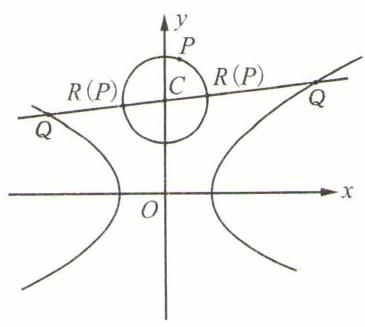
\includegraphics[width=0.3\textwidth]{bodyxb/src/bo_d20cdrf7aajc73bfmvhg_98_1092_205_365_327_0.jpg}
\end{center}


[第 25(4)题]

$\therefore \left| {QP}\right|  \geq  \left| {QR}\right| ,\;\therefore \left| {PQ}\right|$ 最小时, $C,P,Q$ 三点一定共线 (如图),此时 $\left| {PQ}\right|  = \left| {CQ}\right|  - \left| {CR}\right|  = \left| {CQ}\right|  - 1$ ,即 $\left| {PQ}\right|$ 最小时, $\left| {CQ}\right|$ 也应最小,将点 $Q$ 写为参数形式 $Q\left( {\dfrac{1}{\cos \theta },\tan \theta }\right) ,\theta$ 为参数, $\left| {CQ}\right|  = \sqrt{\dfrac{1}{{\cos }^{2}\theta } + {\left( \tan \theta  - 2\right) }^{2}} =$  $\sqrt{2{\tan }^{2}\theta  - 4\tan \theta  + 5} = \sqrt{2{\left( \tan \theta  - 1\right) }^{2} + 3} \geq  \sqrt{3}$ ,等号成立时, $\tan \theta  = 1$ ,对应 $Q\left( {\sqrt{2},1}\right)$ 或 $Q\left( {-\sqrt{2},1}\right)$ . 此时点 $P$ 的坐标为 $P\left( {\dfrac{\sqrt{6}}{3},2 - \dfrac{\sqrt{3}}{3}}\right)$ 或 $P\left( {-\dfrac{\sqrt{6}}{3},2 - \dfrac{\sqrt{3}}{3}}\right) ,{\left| PQ\right| }_{\min } = \sqrt{3} - 1.$

26. (1) 由 $\dfrac{{x}^{2}}{4} + {y}^{2} = 1$ ,将点 $C$ 的坐标写成参数形式: $C\left( {2\cos \theta ,\sin \theta }\right) \left( {\theta \text{ 为参数且 }0 < \theta  < \dfrac{\pi }{2}}\right) ,\left| {OA}\right|  = 2,\left| {OB}\right|  = 1$ .

${S}_{\text{ 四边形 OACB }} = {S}_{\bigtriangleup {BOC}} + {S}_{\bigtriangleup {AOC}} = \dfrac{1}{2} \cdot  \left| {OB}\right|  \cdot  {x}_{C} + \dfrac{1}{2} \cdot  \left| {OA}\right|  \cdot  {y}_{C} = \cos \theta  + \sin \theta  = \sqrt{2}\sin \left( {\theta  + \dfrac{\pi }{4}}\right) ,0 < \theta  < \dfrac{\pi }{2}$ 时,

${S}_{\text{ 四边形 }{OACB}\max } = \sqrt{2}$ ,此时 $\theta  = \dfrac{\pi }{4}$ ,点 $C$ 的坐标为 $C\left( {\sqrt{2},\dfrac{\sqrt{2}}{2}}\right)$ .

(2)将点 $C$ 的坐标写成参数形式 $C\left( {3\cos \theta ,5\sin \theta }\right) \left( {\theta \text{ 是参数 }}\right)$ . 设 $D\left( {{x}_{D},0}\right) ,\left| {CD}\right|  = \sqrt{{\left( {x}_{D} - 3\cos \theta \right) }^{2} + {5}^{2}{\sin }^{2}\theta } = 5$ ,

$\therefore {x}_{D} = 3\cos \theta  \pm  \left| {5\cos \theta }\right|  = 3\cos \theta  \pm  5\cos \theta$ . 当 ${x}_{D} = 8\cos \theta$ 时, $\left\{  \begin{array}{l} {x}_{M} = \dfrac{11}{2}\cos \theta , \\  {y}_{M} = \dfrac{5}{2}\sin \theta , \end{array}\right.$ 此时点 $M$ 的轨迹方程为 $\dfrac{4{x}^{2}}{121} + \dfrac{4{y}^{2}}{25} = 1$ ; 当 ${x}_{D} =  - 2\cos \theta$ 时, $\left\{  \begin{array}{l} {x}_{M} = \dfrac{1}{2}\cos \theta , \\  {y}_{M} = \dfrac{5}{2}\sin \theta , \end{array}\right.$ 此时点 $M$ 的轨迹方程为 $4{x}^{2} + \dfrac{4{y}^{2}}{25} = 1$ .

27. (1) $\because A\left( {t,0}\right) ,\therefore B\left( {t + 1,0}\right) ,{l}_{PA} : y - 0 = \dfrac{1 - 0}{0 - t}\left( {x - t}\right) \left( {t \neq  0}\right) ,\therefore x + {ty} - t = 0\left( {t \neq  0}\right) ,t = 0$ 时, ${l}_{PA} : x = 0$ 可以看作该式的特例, $\therefore \;{l}_{PA} : x + {ty} - t = 0.{l}_{QB} : y - 2 = \dfrac{0 - 2}{t + 1 - {1.7}}\left( {x - {1.7}}\right) \left( {t \neq  {0.7}}\right) ,\;\therefore \;{2x} + \left( {t - {0.7}}\right) y -$  $2\left( {t + 1}\right)  = 0\left( {t \neq  {0.7}}\right) ,t = {0.7}$ 时, ${l}_{QB} : x = {1.7}$ 可以看作该式的特例, $\therefore {l}_{QB} : {2x} + \left( {t - {0.7}}\right) y - 2\left( {t + 1}\right)  = 0$ .

(2)将 ${l}_{PA}$ 改写为 $x = \left( {1 - y}\right) t$ ,将 ${l}_{QB}$ 改写为 $t\left( {2 - y}\right)  = {2x} - {0.7y} - 2$ ,两式相乘消去 $t$ ,得 $x\left( {2 - y}\right)  = \left( {1 - y}\right) ({2x} - {0.7y}$ -2). $\therefore {PA},{QB}$ 交点的轨迹方程为 ${0.7}{y}^{2} - {xy} + {1.3y} - 2 = 0$ .

28. (1) 以点 $O$ 为坐标原点, ${OA}$ 为 $x$ 轴正方向, ${OC}$ 为 $y$ 轴正方向建立平面直角坐标系. 设 $M\left( {0,t}\right) \left( {0 < t < b}\right)$ ,则 $\dfrac{\left| OM\right| }{\left| MC\right| } =$  $\dfrac{t}{b - t} = \dfrac{\left| BN\right| }{\left| NC\right| } = \dfrac{\left| BN\right| }{a - \left| {BN}\right| },\;\therefore \;\left| {BN}\right|  = \dfrac{a}{b} \cdot  t,$

$\therefore N\left( {a - \dfrac{a}{b}t,b}\right)$ . ${l}_{DM} : y = \dfrac{t - 0}{0 + a}\left( {x + a}\right)$ ,即 $y = \dfrac{t}{a}\left( {x + a}\right) ,{l}_{AN} : y = \dfrac{b - 0}{a - \dfrac{a}{b}t - a}\left( {x - a}\right)$ ,即 $y =  - \dfrac{{b}^{2}}{at}\left( {x - a}\right)$ ,联立上述

两个方程,易得 $\left\{  \begin{array}{l} {x}_{P} = \dfrac{a\left( {{b}^{2} - {t}^{2}}\right) }{{b}^{2} + {t}^{2}} = a \cdot  \dfrac{1 - {\left( \dfrac{t}{b}\right) }^{2}}{1 + {\left( \dfrac{t}{b}\right) }^{2}}, \\  {y}_{P} = \dfrac{2{b}^{2}t}{{b}^{2} + {t}^{2}} = b \cdot  \dfrac{2 \cdot  \dfrac{t}{b}}{1 + {\left( \dfrac{t}{b}\right) }^{2}}\text{ . 则 }{\left( \dfrac{1 - {u}^{2}}{1 + {u}^{2}}\right) }^{2} = \dfrac{{\left( 1 + {u}^{2}\right) }^{2}}{{\left( 1 + {u}^{2}\right) }^{2}} = 1,\;\therefore \;{BP}\text{ 的轨迹 } \\  {y}_{P} = \dfrac{2{b}^{2}t}{{b}^{2} + {t}^{2}} = b \cdot  \dfrac{t}{1 + {\left( \dfrac{t}{b}\right) }^{2}}. \end{array}\right.$

方程为 $\dfrac{{x}^{2}}{{a}^{2}} + \dfrac{{y}^{2}}{{b}^{2}} = 1\left( {0 < x < 1,0 < y < 1\text{ ,即在第一象限的部分). }}\right)$

(2)由于点 $P$ 在椭圆的右侧. 故点 $A,B,Q$ 均位于点 $P$ 的左侧. 将过点 $P$ 的直线写成参数方程形式 $l$ : $\left\{  \begin{array}{l} x = 4 + t\cos \alpha , \\  y = 1 + t\sin \alpha  \end{array}\right.$ ( $t$ 是

参数),其中 $\alpha$ 是直线 $l$ 的倾斜角. 将上述方程代入 ${x}^{2} + 2{y}^{2} = 8$ ,整理得 ${t}^{2}\left( {1 + {\sin }^{2}\alpha }\right)  + \left( {8\cos \alpha  + 4\sin \alpha }\right) t + {10} = 0\left( *\right)$ , 当方程 (*) 有解时,不妨设解为 ${t}_{1},{t}_{2}$ ,其中 $A$ 对应参数 ${t}_{1},B$ 对应参数 ${t}_{2}$ ,且 $\left| {t}_{1}\right|  \leq  \left| {t}_{2}\right|$ ,根据参数 $t$ 的几何意义,有 $\lambda$  $=  - \dfrac{\left| {t}_{1}\right| }{\left| {t}_{2}\right| } =  - \dfrac{{t}_{1}}{{t}_{2}}$ . 另一方面, $- \lambda  = \dfrac{\left| \vv{AQ}\right| }{\left| \vv{QB}\right| } = \dfrac{\left| \vv{PQ}\right|  - \left| \vv{PA}\right| }{\left| \vv{PB}\right|  - \left| \vv{PQ}\right| } = \dfrac{\left| \vv{PQ}\right|  - \left| {t}_{1}\right| }{\left| {t}_{2}\right|  - \left| \vv{PQ}\right| }$ . 可解得 $\left| \vv{PQ}\right|  = \dfrac{2\left| {{t}_{1}{t}_{2}}\right| }{\left| {t}_{1}\right|  + \left| {t}_{2}\right| } = \dfrac{2\left| {{t}_{1}{t}_{2}}\right| }{\left| {{t}_{1} + {t}_{2}}\right| }$ ,根据韦达定理, $\left| \vv{PQ}\right|  = 2 \cdot  \dfrac{\dfrac{10}{1 + {\sin }^{2}\alpha }}{\dfrac{\left| 8\cos \alpha  + 4\sin \alpha \right| }{1 + {\sin }^{2}\alpha }} = \dfrac{5}{\left| 2\cos \alpha  + \sin \alpha \right| }$ . 再由参数 $t$ 的几何意义,可知 $\left\{  {\begin{array}{l} {x}_{Q} = 4 + \left( {-\dfrac{5}{2\cos \alpha  + \sin \alpha } \cdot  \cos \alpha }\right) , \\  {y}_{Q} = 1 + \left( {-\dfrac{5}{2\cos \alpha  + \sin \alpha } \cdot  \sin \alpha }\right) , \end{array}\text{ 其中 }{y}_{Q} = 1 - \dfrac{5\sin \alpha }{2\cos \alpha  + \sin \alpha } =  - 4 + \dfrac{{10}\cos \alpha }{2\cos \alpha  + \sin \alpha },\;\therefore \;\dfrac{{x}_{Q} - 4}{-5} = \dfrac{{y}_{Q} + 4}{{10} = {10}} = \dfrac{\cos \alpha }{2\cos \alpha  + \sin \alpha },}\right.$  $\therefore$ 动点 $Q$ 的轨迹方程为 ${2x} + y - 4 = 0$ (在椭圆 ${x}^{2} + 2{y}^{2} = 8$ 内的部分).

29. (1) 直线 ${P}_{1}{P}_{2}$ 是过原点(0,0),倾斜角为 $\alpha$ 的直线,故其参数方程可写为

$\left\{  {\begin{array}{l} x = 0 + t\cos \alpha  = t\cos \alpha , \\  y = 0 + t\sin \alpha  = t\sin \alpha  \end{array}\text{ ( }t}\right.$ 为参数).

(2)将 $\left\{  \begin{array}{l} x = t\cos \alpha , \\  y = t\sin \alpha  \end{array}\right.$ 代入 $y = {x}^{2} - {2x} + 2$ ,整理得 ${t}^{2}{\cos }^{2}\alpha  - \left( {\sin \alpha  + 2\cos \alpha }\right) t + 2 = 0\left( *\right)$ ,方程 (*) 有解时,有 ${t}_{1} + {t}_{2} =$  $\dfrac{\sin \alpha  + 2\cos \alpha }{{\cos }^{2}\alpha },{t}_{1} \cdot  {t}_{2} = \dfrac{2}{{\cos }^{2}\alpha } > 0,\;\therefore \;{t}_{1},{t}_{2}$ 同号,

$\therefore \dfrac{1}{\left| O{P}_{1}\right| } + \dfrac{1}{\left| O{P}_{2}\right| } = \dfrac{1}{\left| {t}_{1}\right| } + \dfrac{1}{\left| {t}_{2}\right| } = \dfrac{2}{\left| OQ\right| },\;\therefore \;\left| {OQ}\right|  = 2 \cdot  \dfrac{\left| {t}_{1}\right|  \cdot  \left| {t}_{2}\right| }{\left| {t}_{1}\right|  + \left| {t}_{2}\right| } = 2 \cdot  \dfrac{{t}_{1} \cdot  {t}_{2}}{\left| {t}_{1} + {t}_{2}\right| } = \dfrac{4}{\left| \sin \alpha  + 2\cos \alpha \right| }.$

显然,点 $Q$ 对应的参数 ${t}_{Q}$ ,与 ${t}_{1},{t}_{2}$ 均同号.

$\therefore \left\{  {\begin{array}{l} {x}_{Q} = \dfrac{4\cos \alpha }{\sin \alpha  + 2\cos \alpha }, \\  {y}_{Q} = \dfrac{4\sin \alpha }{\sin \alpha  + 2\cos \alpha } \end{array}\left( {\alpha \text{ 为参数 }}\right) \text{ . 注意到, }{y}_{Q} = \dfrac{4\sin \alpha  + 8\cos \alpha  - 8\cos \alpha }{\sin \alpha  + 2\cos \alpha } = 4 - \dfrac{8\cos \alpha }{\sin \alpha  + 2\cos \alpha },}\right.$

$\therefore \dfrac{{x}_{Q}}{4} = \dfrac{{y}_{Q} - 4}{-8} = \dfrac{\cos \alpha }{\sin \alpha  + 2\cos \alpha },\therefore 2{x}_{Q} + {y}_{Q} - 4 = 0$ . 另, $\alpha  \in  \left( {0,\dfrac{\pi }{2}}\right)$ 时, $\left( *\right)$ 式的 $\Delta  = {\left( \sin \alpha  + 2\cos \alpha \right) }^{2} - 8{\cos }^{2}\alpha  \geq  0$ ,

$\therefore \sin \alpha  + 2\cos \alpha  \geq  2\sqrt{2}\cos \alpha ,\;\therefore \tan \alpha  \geq  2\sqrt{2} - 2.{x}_{Q} = \dfrac{4\cos \alpha }{\sin \alpha  + 2\cos \alpha } = \dfrac{4}{\tan \alpha  + 2} \leq  \sqrt{2}$ ,

$\therefore$ 当 $\alpha$ 在区间 $\left( {0,\dfrac{\pi }{2}}\right)$ 内变动时,点 $Q$ 轨迹的普通方程为 ${2x} + y - 4 = 0\left( {0 < x \leq  \sqrt{2}}\right)$ .

30. 将直线 ${OQ}$ 写成参数方程的形式 $\left\{  {\begin{array}{l} x = t\cos \theta , \\  y = t\sin \theta  \end{array}\left( {t\text{ 是参数 }}\right) \left( {\theta  \in  \lbrack 0,\pi )}\right) }\right.$ ,代入 ${x}^{2} + {\left( y - 1\right) }^{2} = 1$ ,整理得 ${t}^{2} - {2t}\sin \theta  = 0$ ,

$\therefore {t}_{1} = 0,{t}_{2} = 2\sin \theta .{t}_{1}$ 对应 $O\left( {0,0}\right) ,{t}_{2}$ 对应 $Q\left( {2\sin \theta \cos \theta ,2{\sin }^{2}\theta }\right)$ ,点 $P$ 的坐标可以写成 $\left( {{t}_{P}\cos \theta ,{t}_{P}\sin \theta }\right)$ ,为找到所有符合条件的点 $P$ ,需求解如下方程 ${\left| PQ\right| }^{2} = {\left( {t}_{P} - {t}_{Q}\right) }^{2} = {\left( {t}_{P} - 2\sin \theta \right) }^{2} = {\left| {y}_{P} - 2\right| }^{2} = {\left( {t}_{P}\sin \theta  - 2\right) }^{2}$ ,整理为关于 ${t}_{P}$ 的方程 ${\cos }^{2}\theta  \cdot  {t}_{P}^{2} - 4{\cos }^{2}\theta  = 0$ . 讨论:①当 ${\cos }^{2}\theta  = 0$ 即 $\cos \theta  = 0$ 时, $\because \theta  \in  \lbrack 0,\pi ),\therefore \theta  = \dfrac{\pi }{2}$ ,此时,直线 ${OQ}$ 即直线 $x =$ 0,点 $Q$ 的坐标为 $Q\left( {0,2}\right) ,Q$ 在直线 $y = 2$ 上,且直线 $x = 0$ 和 $y = 2$ 互相垂直,此时直线 $x = 0$ 上的任意一点,均满足到直线 $y = 2$ 的距离等于到点 $Q$ 的距离. ②当 ${\cos }^{2}\theta  \neq  0$ ,即 $\theta  \in  \left\lbrack  {0,\dfrac{\pi }{2}}\right)  \cup  \left( {\dfrac{\pi }{2},\pi }\right)$ 时, ${t}_{P}^{2} = 4$ ,故 ${t}_{P} =  \pm  2$ ,此时 $\left\{  \begin{array}{l} {x}_{P} = 2\cos \theta , \\  {y}_{P} = 2\sin \theta , \end{array}\right.$ 点 $P$ 的轨迹为 ${x}^{2} + {y}^{2} = 4\left( {x \neq  0}\right)$ . 特别地, $x = 0$ 时, $y =  \pm  2$ ,是讨论情况 ① 的特例. 综上,点 $P$ 的轨迹是圆 ${x}^{2} + {y}^{2} = 4$ 和直线 $x = 0$ .

\begin{center}
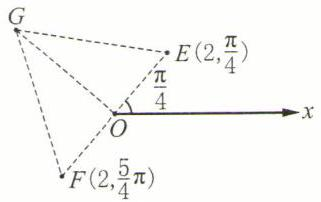
\includegraphics[width=0.2\textwidth]{bodyxb/src/bo_d20cdrf7aajc73bfmvhg_99_1118_1720_321_202_0.jpg}
\end{center}


(第 31 题)

31. B 提示: 如图,由题意, $E,O,F$ 三点共线. 又 $\because \bigtriangleup {EFG}$ 为等边三角形,

$\therefore {GO} \bot  {EF}$ ,且易知 $\left| {GO}\right|  = \left| {EO}\right|  \cdot  \cot {30}^{ \circ  } = 2\sqrt{3},\angle {GOx} = \dfrac{\pi }{4} + \dfrac{\pi }{2} = \dfrac{3\pi }{4},\;\therefore$ 点 $G$ 的极坐标为 $\left( {2\sqrt{3},\dfrac{3}{4}\pi  + {2k\pi }}\right) \left( {k \in  \mathbf{Z}}\right)$ ,即可能是 $\left( {2\sqrt{3},\dfrac{3}{4}\pi }\right)$ .

32. C 提示: 用坐标变换公式 $\left\{  \begin{array}{l} x = \rho \cos \theta , \\  y = \rho \sin \theta  \end{array}\right.$ 将备选答案写成直角坐标. 对于选项 A,变换后为(3, - 4); 对于选项 B,变换后为 (3,4)；对于选项 $C$ ,变换后为(-3,4)；对于选项 $D$ ,变换后为(3, - 4),故选 $C$ .

33. A 提示,方法一:由 $\sin \theta  = \dfrac{1}{3}$ ,得 $\rho \sin \theta  = \dfrac{1}{3}\rho$ . 又 $\rho  \in  \mathbf{R}$ . $\therefore y =  \pm  \dfrac{1}{3}\sqrt{{x}^{2} + {y}^{2}}$ ,整理得 $x \pm  2\sqrt{2}y = 0$ 是两条相交直

线,交点是极点 (原点). 方法二: 三角方程 $\sin \theta  = \dfrac{1}{3}$ 的解是 $\theta  = \arcsin \dfrac{1}{3} + 2{k}_{1}\pi$ 或 $\theta  = \pi  - \arcsin \dfrac{1}{3} + 2{k}_{2}\pi \left( {{k}_{1},{k}_{2} \in  \mathbf{Z}}\right)$ ,又 $\rho  \in  \mathbf{R}$ ,故 $\sin \theta  = \dfrac{1}{3}$ 代表过极点的两条相交直线.

34. $C$ 提示: 圆在直角坐标系中的方程为 ${\left( x - 1\right) }^{2} + {y}^{2} = 1$ ,即 ${x}^{2} + {y}^{2} - {2x} = 0$ ,把 $\left\{  \begin{array}{l} x = \rho \cos \theta , \\  y = \rho \sin \theta  \end{array}\right.$ 代入,

$\therefore {\rho }^{2} - {2\rho }\cos \theta  = 0,\therefore \rho  = 0$ 或 $\rho  = 2\cos \theta$ . 特别注意, $\rho  = 0$ 对应的是极点,而极点坐标的极角可以是任意的,例如 $\left( {0,\dfrac{\pi }{2}}\right)$ ,包含在 $\rho  = 2\cos \theta$ 的解集之中.

35. D 提示: $\because {\sin }^{2}\dfrac{\theta }{2} = \dfrac{1 - \cos \theta }{2},\therefore$ 曲线方程可写为 $\rho  = \dfrac{\dfrac{2}{3}}{1 - \cos \theta }$ . 同例 2,判定这是抛物线.

36. $C$ 提示: $\because \rho  = a\cos \theta  + b\sin \theta ,\;\therefore {\rho }^{2} = {a\rho }\cos \theta  + {b\rho }\sin \theta$ ,在直角坐标系中,有 ${x}^{2} + {y}^{2} = {ax} + {by}$ ,即 ${\left( x - \dfrac{a}{2}\right) }^{2} +$  ${\left( y - \dfrac{b}{2}\right) }^{2} = \dfrac{1}{4}\left( {{a}^{2} + {b}^{2}}\right)$ ,其与 $y = 0$ (对应极轴) 相切的充要条件是 $\left\{  {\begin{array}{l} \dfrac{1}{4}\left( {{a}^{2} + {b}^{2}}\right)  > 0, \\  \left| \dfrac{b}{2}\right|  = \sqrt{\dfrac{1}{4}\left( {{a}^{2} + {b}^{2}}\right) } \end{array} \Leftrightarrow  a = 0,b \neq  0}\right.$ .

$* {37}$ . D 提示: 将原方程视为关于 $\rho$ 的二次方程,有解 $\rho  = \theta$ 或 $\rho  = 3$ ,分别是一条等速螺线和一个圆. 注: 极坐标方程 $\rho  = {a\theta }(a >$ 0),即为等速螺线,或称阿基米德螺线,其特点是一条射线上的动点在沿着该射线作匀速运动的同时,射线又绕着它的端点作等角速度旋转, 此时动点的轨迹就是等速螺线.

38. (1) $\sqrt{{25} - {12}\sqrt{3}}\;3$ 提示:点 $A,B$ 在平面直角坐标系中对应 $A\left( {\dfrac{3}{2},\dfrac{3}{2}\sqrt{3}}\right) ,B\left( {2\sqrt{3},2}\right) ,\therefore \left| {AB}\right|  =$  $\sqrt{{\left( 2\sqrt{3} - \dfrac{3}{2}\right) }^{2} + {\left( 2 - \dfrac{3}{2}\sqrt{3}\right) }^{2}} = \sqrt{{25} - {12}\sqrt{3}} \cdot  \vv{OA} \cdot  \vv{OB} = 6\sqrt{3} = \left| \vv{OA}\right|  \cdot  \left| \vv{OB}\right|  \cdot  \cos \angle {AOB} = 3 \times  4 \cdot  \cos \angle {AOB},$  $\therefore \cos \angle {AOB} = \dfrac{\sqrt{3}}{2},{S}_{\bigtriangleup {AOB}} = \dfrac{1}{2} \cdot  \left| \vv{OA}\right|  \cdot  \left| \vv{OB}\right|  \cdot  \sin \angle {AOB} = \dfrac{1}{2} \cdot  3 \cdot  4 \cdot  \dfrac{1}{2} = 3$ . (2) $\dfrac{8}{3}\pi$ 提示: $\theta  = 0,\theta  = \dfrac{\pi }{3}\left( {\rho  \geq  0}\right)$ 是以极点为端点,极角分别为 0, $\dfrac{\pi }{3}$ 的两条射线； $\rho  = 4$ 是以极点为圆心,4 为半径的圆,围成的图形是一个扇形,其面积 $S = \dfrac{\dfrac{\pi }{3}}{2\pi } \cdot  \pi  \cdot  {4}^{2} = \dfrac{8}{3}\pi$ .

(3) $\dfrac{3}{2}$ 提示:均写成平面直角坐标形式:直线 $\rho \sin \theta  = 3 \Rightarrow  y = 3$ ,圆 $\rho  = 3\sin \theta$ 即 ${\rho }^{2} = {3\rho }\sin \theta  \Rightarrow  {x}^{2} + {y}^{2} = {3y}$ ,其圆心为 $\left( {0,\dfrac{3}{2}}\right) ,\;\therefore \;$ 圆心到直线 $y = 3$ 的距离为 $\left| {3 - \dfrac{3}{2}}\right|  = \dfrac{3}{2}$ .

(4) $\left( {\dfrac{5}{2},\arctan \dfrac{4}{3}}\right) \dfrac{5}{2}$ 提示:先写成平面直角坐标形式. $\because {\rho }^{2} = {3\rho }\cos \theta  + {4\rho }\sin \theta$ ,

$\therefore {x}^{2} + {y}^{2} = {3x} + {4y},\therefore {\left( x - \dfrac{3}{2}\right) }^{2} + {\left( y - 2\right) }^{2} = {\left( \dfrac{5}{2}\right) }^{2}$ ,圆心 $\left( {\dfrac{3}{2},2}\right)$ 的极坐标是 $\left( {\dfrac{5}{2},\arctan \dfrac{4}{3}}\right)$ ,半径为 $\dfrac{5}{2}$ .

(5) ① $\left( {2, - \dfrac{11}{7}\pi }\right)$ ② $\left( {-2,\dfrac{10}{7}\pi }\right)$ 提示:① $\rho  > 0$ 时, $P\left( {2,\dfrac{3}{7}\pi }\right)$ 也可写成 $P\left( {2,\dfrac{3}{7}\pi  + {2k\pi }}\right) \left( {k \in  \mathbf{Z}}\right)$ .

$\because  - {2\pi } < \theta  < 0,\;\therefore \;k =  - 1$ ,即 $\left( {2, - \dfrac{11}{7}\pi }\right)$ .

② $\rho  < 0$ 时, $P\left( {2,\dfrac{3}{7}\pi }\right)$ 也可写成 $P\left( {-2,\dfrac{3}{7}\pi  + \left( {{2k} + 1}\right) \pi }\right) \left( {k \in  \mathbf{Z}}\right)$ .

$\because 0 \leq  \theta  < {2\pi },\;\therefore \;k = 0$ ,即 $\left( {-2,\dfrac{10}{7}\pi }\right)$ .

39. $\left( {\rho ,\theta }\right)$ 关于极轴、极点、直线 $\theta  = \dfrac{\pi }{2}\left( {\rho  \in  \mathbf{R}}\right)$ 、直线 $\theta  = \dfrac{\pi }{4}\left( {\rho  \in  \mathbf{R}}\right)$ 对称的点分别为 $\left( {\rho , - \theta }\right) ,\left( {-\rho ,\theta }\right)$ , $\left( {\rho ,\pi  - \theta }\right) ,\left( {\rho ,\dfrac{\pi }{2} - \theta }\right)$ .

(1) $\because \rho  > 0, - \pi  \leq  \theta  < \pi ,\therefore$ 点 $\left( {2,\dfrac{\pi }{6}}\right)$ 关于极轴对称的点为 $\left( {2, - \dfrac{\pi }{6}}\right)$ ；关于极点对称的点为 $\left( {2, - \dfrac{5\pi }{6}}\right)$ ；关于直线 $\theta$  $= \dfrac{\pi }{2}\left( {\rho  \in  \mathbf{R}}\right)$ 对称的点为 $\left( {2,\dfrac{5\pi }{6}}\right)$ : 关于直线 $\theta  = \dfrac{\pi }{4}\left( {\rho  \in  \mathbf{R}}\right)$ 对称的点为 $\left( {2,\dfrac{\pi }{3}}\right)$ .

(2)若 $\left( {\rho ,\theta }\right)$ 在曲线 ${C}_{1} : \rho  = \dfrac{4}{2\cos \theta  + 3\sin \theta }$ 上,则 $\left\{  \begin{array}{l} {\rho }^{\prime } = \rho , \\  {\theta }^{\prime } =  - \theta  \end{array}\right.$ 在 ${C}_{1}$ 关于极轴对称的曲线 ${C}_{1}^{\prime }$ 上, $\therefore \;{\rho }^{\prime } =$  $\dfrac{4}{2\cos \left( {-{\theta }^{\prime }}\right)  + 3\sin \left( {-{\theta }^{\prime }}\right) } = \dfrac{4}{2\cos {\theta }^{\prime } - 3\sin {\theta }^{\prime }},\therefore {C}^{\prime } : \rho  = \dfrac{4}{2\cos \theta  - 3\sin \theta }$ . 类似地,曲线关于极点对称的曲线满足 $- \rho$  $= \dfrac{4}{2\cos \theta  + 3\sin \theta },\;\therefore \rho  =  - \dfrac{4}{2\cos \theta  + 3\sin \theta }$ . 关于直线 $\theta  = \dfrac{\pi }{2}\left( {\rho  \in  \mathbf{R}}\right)$ 对称的曲线满足 $\rho  = \dfrac{4}{2\cos \left( {\pi  - \theta }\right)  + 3\sin \left( {\pi  - \theta }\right) }$ , $\therefore \rho  = \dfrac{4}{3\sin \theta  - 2\cos \theta }$ . 关于直线 $\theta  = \dfrac{\pi }{4}\left( {\rho  \in  \mathbf{R}}\right)$ 对称的曲线满足 $\rho  = \dfrac{4}{2\cos \left( {\dfrac{\pi }{2} - \theta }\right)  + 3\sin \left( {\dfrac{\pi }{2} - \theta }\right) },\;\therefore \rho  =$  $\dfrac{4}{2\sin \theta  + 3\cos \theta }$ . 注:由于极坐标系上的点与极坐标并不一一对应 (如 $\left( {{2\pi },\pi }\right)$ 与 $\left( {{2\pi },{3\pi }}\right)$ 是同一点,但只有前者满足等距螺线方程 $\rho  = {2\theta })$ ,因此,如果认为 $\left( {\rho ,\theta }\right)$ 在关于极轴对称的曲线上,而 $\left( {\rho , - \theta }\right)$ 在原曲线上,并代入原曲线的论述是不严谨的,这是极坐标系与直角坐标系的一大不同,请读者特别留意.

40. (1) ${y}^{2} = 4\left( {x + 1}\right)$ 提示: $\because \rho {\sin }^{2}\dfrac{\theta }{2} = 1,\therefore \rho \dfrac{1 - \cos \theta }{2} = 1,\therefore \sqrt{{x}^{2} + {y}^{2}} - x = 2$ ,整理得 ${y}^{2} = 4\left( {x + 1}\right)$ .

(2) ${x}^{2} + {y}^{2} = 0$ 或 $x = 1$ 提示: $\because {\rho }^{2}\cos \theta  - \rho  = 0,\therefore \rho  = 0$ 或 $\rho \cos \theta  = 1$ ,即 ${x}^{2} + {y}^{2} = 0$ 或 $x = 1$ .

(3) $y = \left| x\right| \left( {x \neq  0}\right)$ 提示:方法一:三角方程 $\sin \theta  = \dfrac{\sqrt{2}}{2}$ 的解为 ${\theta }_{1} = \dfrac{\pi }{4} + 2{k}_{1}\pi ,{\theta }_{2} = \dfrac{3\pi }{4} + 2{k}_{2}\pi \left( {{k}_{1},{k}_{2} \in  \mathbf{Z}}\right)$ . 又 $\rho  > 0$ ,故 $\sin \theta  = \dfrac{\sqrt{2}}{2}$ 代表 $y = x\left( {x > 0}\right)$ 或 $y =  - x\left( {x < 0}\right)$ ,即: $y = \left| x\right| \left( {x \neq  0}\right)$ . 方法二: $\because \sin \theta  = \dfrac{\sqrt{2}}{2},\rho  > 0,\;\therefore \rho \sin \theta  = \dfrac{\sqrt{2}}{2}\rho$  $> 0,\;\therefore \;y = \dfrac{\sqrt{2}}{2}\sqrt{{x}^{2} + {y}^{2}}$ 且 $y > 0$ ,整理得 ${y}^{2} = {x}^{2}$ ,即 $y = \left| x\right| \left( {x \neq  0}\right)$ .

(4) ${\left( x - \dfrac{1}{2}\right) }^{2} + {\left( y - 1\right) }^{2} = \dfrac{5}{4}$ 提示: $\because \rho  = \cos \theta  + 2\sin \theta ,\therefore {\rho }^{2} = \rho \cos \theta  + {2\rho }\sin \theta ,\therefore {x}^{2} + {y}^{2} = x + {2y}$ ,即 ${x}^{2}$  $+ {y}^{2} - x - {2y} = 0,{\left( x - \dfrac{1}{2}\right) }^{2} + {\left( y - 1\right) }^{2} = \dfrac{5}{4}$ .

(5) $x + 6 = 0$ 提示:已知即为 $\rho \cos \theta  + 6 = 0,\;\therefore \;x + 6 = 0$ .

(6) ${y}^{2} - \dfrac{{x}^{2}}{4} = 1\left( {x \neq  0}\right)$ 提示:由题意, $\theta  \neq  \dfrac{\pi }{2} + {k\pi }\left( {k \in  \mathbf{Z}}\right) ,\;\therefore \;{x}^{2} = 4\left( {{y}^{2} - 1}\right)$ ,即 ${y}^{2} - \dfrac{{x}^{2}}{4} = 1\left( {x \neq  0}\right)$ .

(7) ${x}^{2} + {y}^{2} = {36}$ 或 ${x}^{2} + {y}^{2} = 1$ 提示: $\because {\rho }^{2} - {5\rho } - 6 = 0$ 且 $\rho  \in  \mathbf{R},\;\therefore \rho  = 6$ 或 $\rho  =  - 1,\;\therefore {x}^{2} + {y}^{2} = {36}$ 或 ${x}^{2} +$  ${y}^{2} = 1$ .

41. (1) 将直线和圆写成直角坐标方程的形式,直线: ${ax} + {by} = 1$ ,圆: ${x}^{2} + {y}^{2} = {2cx}$ ,即 ${\left( x - c\right) }^{2} + {y}^{2} = {c}^{2}$ . 直线与圆相切的充要条件是圆心到直线的距离等于半径,

$\therefore \dfrac{\left| a \cdot  c + b \cdot  0 - 1\right| }{\sqrt{{a}^{2} + {b}^{2}}} = c,\;\therefore \;{b}^{2}{c}^{2} + {2ac} = 1$ ,证毕.

(2)将抛物线 $\rho  = \dfrac{8\cos \theta }{{\sin }^{2}\theta }\left( {\theta  \neq  0}\right)$ 写成直角坐标方程的形式: ${y}^{2} = {8x}\left( {x \neq  0}\right)$ ,准线为 $x =  - 2$ . 点 $M$ 的坐标满足: $\sqrt{{x}_{M}^{2} + {y}_{M}^{2}}$  $= {x}_{M} - \left( {-2}\right)$ ,代入 ${y}_{M}^{2} = 8{x}_{M}$ ,可得 ${x}_{M} = 1,{y}_{M} =  \pm  2\sqrt{2}$ . (或:点 $M$ 的极径 $= \left| {OM}\right|$ ,点 $M$ 到准线的距离 $=$ 点 $M$ 到焦点 $F\left( {2,0}\right)$ 的距离 $\left| {FM}\right|$ ,故点 $M$ 在线段 ${OF}$ 的垂直平分线 $x = 1$ 上,故 ${x}_{M} = 1,{y}_{M} =  \pm  2\sqrt{2}$ ). $\because \rho  > 0, - \pi  \leq  \theta  < \pi ,\;\therefore \;$ 点 $M$ 的极坐标为 $M\left( {3, \pm  \arctan 2\sqrt{2}}\right)$ .

(3)将两圆写成直角坐标方程的形式: $\rho  = 2\cos \theta  \Rightarrow  {x}^{2} + {y}^{2} = {2x}$ ,即 ${\left( x - 1\right) }^{2} + {y}^{2} = 1$ ,记圆心 ${C}_{1}\left( {1,0}\right)$ ,半径 ${r}_{1} = 1$ ； ${\rho }^{2} - 2\sqrt{3}\rho \sin \theta  + 2 = 0 \Rightarrow  {x}^{2} + {y}^{2} - 2\sqrt{3}y + 2 = 0$ ,即 ${x}^{2} + {\left( y - \sqrt{3}\right) }^{2} = 1$ ,记圆心 ${C}_{2}\left( {0,\sqrt{3}}\right)$ ,半径 ${r}_{2} = 1$ . $\left| {{C}_{1}{C}_{2}}\right|  = \sqrt{{1}^{2} + {\left( \sqrt{3}\right) }^{2}} = 2 = {r}_{1} + {r}_{2},\;\therefore \;$ 两圆外切. 又 $\because {r}_{1} = {r}_{2}$ ,故切点恰好为线段 ${C}_{1}{C}_{2}$ 的中点,即 $\left( {\dfrac{1}{2},\dfrac{\sqrt{3}}{2}}\right)$ ,极坐标为 $\left( {1,\dfrac{\pi }{3}}\right)$ .

42. D 提示: 由题意, $Q\left( {{\rho }_{2},{\theta }_{2}}\right)$ 可写为 $Q\left( {-{\rho }_{1}, - {\theta }_{1}}\right)$ ,即 $Q\left( {{\rho }_{1}, - {\theta }_{1} + \pi }\right) ,\therefore$ 点 $P,Q$ 关于直线 $\theta  = \dfrac{\pi }{2}$ 对称.

43. B 提示: 曲线 $\rho  = 5\sqrt{3}\cos \theta  - 5\sin \theta$ 上的点 $\left( {\rho ,\theta }\right)$ 关于极轴对称的点为 $\left\{  \begin{array}{l} {\rho }^{\prime } = \rho , \\  {\theta }^{\prime } =  - \theta , \end{array}\right.$

$\therefore$ 曲线 $C : {\rho }^{\prime } = 5\sqrt{3}\cos \left( {-{\theta }^{\prime }}\right)  - 5\sin \left( {-{\theta }^{\prime }}\right)  = 5\sqrt{3}\cos {\theta }^{\prime } + 5\sin {\theta }^{\prime } = {10}\sin \left( {{\theta }^{\prime } + \dfrac{\pi }{3}}\right)$ ,

$\therefore$ 曲线 $C : \rho  = {10}\sin \left( {\theta  + \dfrac{\pi }{3}}\right)  = {10}\cos \left( {\theta  - \dfrac{\pi }{6}}\right)$ .

44. C 提示: $\sin \theta  =  - \dfrac{1}{2},\therefore {\theta }_{1} = \dfrac{11}{6}\pi  + 2{k}_{1}\pi ,{\theta }_{2} = \dfrac{7}{6}\pi  + 2{k}_{2}\pi \left( {{k}_{1},{k}_{2} \in  \mathbf{Z}}\right) ;\cos \theta  = \dfrac{\sqrt{3}}{2},\therefore {\theta }_{3} = \dfrac{11}{6}\pi  + 2{k}_{3}\pi ,{\theta }_{4} = \dfrac{1}{6}\pi  +$  $2{k}_{4}\pi \left( {{k}_{3},{k}_{4} \in  \mathbf{Z}}\right)$ . 又 $\because \rho  \in  \mathbf{R}$ ,故对于每一个 $\left( {\rho ,{\theta }_{4}}\right)$ 可以写成 $\left( {-\rho ,{\theta }_{4} + \pi }\right)$ 的形式,而 ${\theta }_{4} + \pi  = \dfrac{7}{6}\pi  + 2{k}_{4}\pi \left( {{k}_{4} \in  \mathbf{Z}}\right)$ 与 ${\theta }_{2}$ 的形式一致. 故 $P = S$ .

45. $\mathrm{{BD}}$ 提示: $\rho \cos \left( {\theta  - \alpha }\right)  = \rho \cos \theta \cos \alpha  + \rho \sin \theta \sin \alpha ,\therefore$ 圆方程的直角坐标形式为 ${x}^{2} + {y}^{2} - {2a}\left( {x\cos \alpha  + y\sin \alpha }\right)  + {a}^{2} - {r}^{2} = 0$ , 即 ${\left( x - a\cos \alpha \right) }^{2} + {\left( y - a\sin \alpha \right) }^{2} = {r}^{2}\left( *\right)$ ,需与 $y = 0$ 相切且切点为(0,0).

$\therefore a\cos \alpha  = 0,\left| {a\sin \alpha }\right|  = r,\;\therefore a = r$ ,且 $\sin \alpha  =  \pm  1,\alpha  \in  \lbrack 0,{2\pi })$ 有解 $\alpha  = \dfrac{\pi }{2}$ 或 $\alpha  = \dfrac{3\pi }{2}$ ,均满足题意.

* 46. (1) $\rho  = {20} + \dfrac{5}{2\pi } \cdot  \theta \left( {0 \leq  \theta  \leq  {6\pi }}\right)$ 提示: 由题意,设曲线方程为 $\rho  = {\rho }_{0} + {a\theta }\left( {0 \leq  \theta  \leq  {6\pi }}\right)$ ,代入 $\left( {{20},0}\right) ,\left( {{35},{6\pi }}\right)$ ,得 $\left\{  {\begin{array}{l} {20} = {\rho }_{0}, \\  {35} = {\rho }_{0} + a \cdot  {6\pi }, \end{array}\;\therefore \;\left\{  {\begin{array}{l} {\rho }_{0} = {20}, \\  a = \dfrac{5}{2\pi }, \end{array}\;\therefore \;\rho  = {20} + \dfrac{5}{2\pi } \cdot  \theta \left( {0 \leq  \theta  \leq  {6\pi }}\right) .}\right. }\right.$

(2) $\rho  = {20} + \dfrac{12}{\pi } \cdot  \theta$ 提示:由题意,设曲线方程为 $\rho  = {\rho }_{0} + {a\theta }$ ,代入 ${P}_{1},{P}_{2}$ ,有 $\left\{  {\begin{array}{l} {22} = {\rho }_{0} + a \cdot  \dfrac{\pi }{6}, \\  {44} = {\rho }_{0} + a \cdot  {2\pi }, \end{array}\therefore \left\{  \begin{array}{l} {\rho }_{0} = {20}, \\  a = \dfrac{12}{\pi }, \end{array}\right. }\right.$

$\therefore \;$ 曲线方程为 $\rho  = {20} + \dfrac{12}{\pi } \cdot  \theta$ .

47. (1) 点 $\left( {3,\dfrac{\pi }{3}}\right) ,\left( {3,\dfrac{\pi }{6}}\right)$ 对应的直角坐标为 $\left( {\dfrac{3}{2},\dfrac{3}{2}\sqrt{3}}\right) ,\left( {\dfrac{3}{2}\sqrt{3},\dfrac{3}{2}}\right)$ ,直线在直角坐标系中的方程为 $y - \dfrac{3}{2}\sqrt{3} =$  $\dfrac{\dfrac{3}{2} - \dfrac{3}{2}\sqrt{3}}{\dfrac{3}{2}\sqrt{3} - \dfrac{3}{2}} \cdot  \left( {x - \dfrac{3}{2}}\right)$ ,即 $x + y = \dfrac{3}{2}\left( {1 + \sqrt{3}}\right)$ ,其极坐标形式为 $\rho \cos \theta  + \rho \sin \theta  = \dfrac{3}{2}\left( {1 + \sqrt{3}}\right)$ .

(2)由题意,圆的半径是 $\left| {\rho }_{0}\right|$ ,在直角坐标系中,有圆的方程: ${\left( x - {\rho }_{0}\cos {\theta }_{0}\right) }^{2} + {\left( y - {\rho }_{0}\sin {\theta }_{0}\right) }^{2} = {\rho }_{0}^{2},\;\therefore {x}^{2} + {y}^{2} -$  $2{\rho }_{0}\left( {x \cdot  \cos {\theta }_{0} + y \cdot  \sin {\theta }_{0}}\right)  = 0$ ,其极坐标形式为 ${\rho }^{2} - 2{\rho }_{0}\rho \left( {\cos \theta  \cdot  \cos {\theta }_{0} + \sin \theta  \cdot  \sin {\theta }_{0}}\right)  = 0.\;\because \;\rho  \neq  0,\;\therefore \;\rho  =$  $2{\rho }_{0}\cos \left( {\theta  - {\theta }_{0}}\right)$ .

(3)在直角坐标系中,圆的方程为 ${\left( x - {\rho }_{0}\cos {\theta }_{0}\right) }^{2} + {\left( y - {\rho }_{0}\sin {\theta }_{0}\right) }^{2} = {R}^{2}$ ,代入 $\left\{  \begin{array}{l} x = \rho \cos \theta , \\  y = \rho \sin \theta , \end{array}\right.$ 整理得 ${\rho }^{2} - {2\rho }{\rho }_{0}\cos \left( {\theta  - {\theta }_{0}}\right)  + {\rho }_{0}^{2}$  $- {R}^{2} = 0$ .

48. 以 $O$ 为极点,射线 ${Ox}$ 为极轴建立的极坐标系中,椭圆方程可写为 $\dfrac{1}{{\rho }^{2}} = \dfrac{{\cos }^{2}\theta }{{a}^{2}} + \dfrac{{\sin }^{2}\theta }{{b}^{2}}$ .

(1) 由题意,若点 $B$ 的极坐标为 $\left( {{\rho }_{1},{\theta }_{1}}\right)$ ,则点 $A$ 的极坐标为 $\left( {{\rho }_{2},{\theta }_{1} + \dfrac{\pi }{2}}\right) .\;\therefore \;\dfrac{1}{{\left| OA\right| }^{2}} + \dfrac{1}{{\left| OB\right| }^{2}} = \dfrac{1}{{\rho }_{2}^{2}} + \dfrac{1}{{\rho }_{1}^{2}} =$  $\dfrac{{\cos }^{2}\left( {{\theta }_{1} + \dfrac{\pi }{2}}\right) }{{a}^{2}} + \dfrac{{\sin }^{2}\left( {{\theta }_{1} + \dfrac{\pi }{2}}\right) }{{b}^{2}} + \dfrac{{\cos }^{2}{\theta }_{1}}{{a}^{2}} + \dfrac{{\sin }^{2}{\theta }_{1}}{{b}^{2}} = \dfrac{1}{{a}^{2}} + \dfrac{1}{{b}^{2}} = \dfrac{{a}^{2} + {b}^{2}}{{a}^{2}{b}^{2}}$ ,为定值,证毕.

(2)设直线 ${AB}$ 的方程为 ${Ax} + {By} + C = 0$ ,于是,点 $O$ 到直线 ${AB}$ 的距离为 $\dfrac{\left| C\right| }{\sqrt{{A}^{2} + {B}^{2}}}$ . 将点 $A,B$ 的坐标代入 ${Ax} + {By}$  $+ C = 0$ ,得

$\left\{  {\begin{array}{l} A{\rho }_{1}\cos {\theta }_{1} + B{\rho }_{1}\sin {\theta }_{1} + C = 0, \\  A{\rho }_{2}\cos \left( {{\theta }_{1} + \dfrac{\pi }{2}}\right)  + B{\rho }_{2}\sin \left( {{\theta }_{1} + \dfrac{\pi }{2}}\right)  + C = 0, \end{array}\therefore \left\{  {\begin{array}{l} A\cos {\theta }_{1} + B\sin {\theta }_{1} =  - \dfrac{C}{{\rho }_{1}}, \\   - A\sin {\theta }_{1} + B\cos {\theta }_{1} =  - \dfrac{C}{{\rho }_{2}}, \end{array}\text{ 两式平方后相加,得 }{A}^{2} + {B}^{2} = }\right. }\right.$  ${C}^{2}\left( {\dfrac{1}{{\rho }_{1}^{2}} + \dfrac{1}{{\rho }_{2}^{2}}}\right)$ . 由( 1 )知 $\dfrac{1}{{\rho }_{1}^{2}} + \dfrac{1}{{\rho }_{2}^{2}} = \dfrac{{a}^{2} + {b}^{2}}{{a}^{2}{b}^{2}},\;\therefore \;\dfrac{\left| C\right| }{\sqrt{{A}^{2} + {B}^{2}}} = \dfrac{1}{\sqrt{\dfrac{1}{{\rho }_{1}^{2}} + \dfrac{1}{{\rho }_{2}^{2}}}} = \dfrac{ab}{\sqrt{{a}^{2} + {b}^{2}}}$ ,为定值,证毕.

49. (1) 方法一: 在平面直角坐标系中,设点 $P$ 的坐标为 $P\left( {t,2}\right) \left( {t \in  \mathbf{R}}\right)$ ,不难写出 ${l}_{OP} : {2x} - {ty} = 0$ . 又 $\left| {OP}\right|  = \sqrt{{t}^{2} + 4}$ ,

$\therefore \left| {OQ}\right|  = \dfrac{1}{\sqrt{{t}^{2} + 4}}$ . 可列 $\left\{  \begin{array}{l} 2{x}_{Q} - t \cdot  {y}_{Q} = 0, \\  \sqrt{{x}_{Q}^{2} + {y}_{Q}^{2}} = \left| {OQ}\right|  = \dfrac{1}{\sqrt{{t}^{2} + 4}}, \end{array}\right.$ 解得 $\left\{  {\begin{array}{l} {x}_{Q} = \dfrac{t}{{t}^{2} + 4}, \\  {y}_{Q} = \dfrac{2}{{t}^{2} + 4}. \end{array}\;\because t \in  \mathbf{R},\;\therefore \; - \dfrac{1}{4} \leq  {x}_{Q} \leq  \dfrac{1}{4},0 < }\right.$

${y}_{Q} \leq  \dfrac{1}{2}$ . 将 $t = \dfrac{2{x}_{Q}}{{y}_{Q}}$ 代入 ${y}_{Q} = \dfrac{2}{{t}^{2} + 4}$ ,整理得 ${x}^{2} + {y}^{2} = \dfrac{1}{2}y\left( {y \neq  0}\right)$ . 对应极坐标方程为 ${\rho }^{2} = \dfrac{1}{2}\rho \sin \theta ,\because y \neq  0$ ,

$\therefore \rho  \neq  0,\;\therefore \;$ 点 $Q$ 的轨迹方程为 $\rho  = \dfrac{1}{2}\sin \theta \left( {0 < \theta  < \pi }\right)$ .

方法二:考察 $\rho  > 0,0 < \theta  < \pi$ 的情况,显然,点 $Q$ 的极角与点 $P$ 相同,即 ${\theta }_{P} = {\theta }_{Q}$ ,而点 $P,Q$ 的极径为 $\left| {OP}\right| ,\left| {OQ}\right|$ ,故 ${\rho }_{P}$  ${\rho }_{Q} = 1$ . $\because {\rho }_{P} \cdot  \sin {\theta }_{P} = 2,\;\therefore \;\dfrac{1}{{\rho }_{Q}} \cdot  \sin {\theta }_{Q} = 2,\;\therefore \;$ 点 $Q$ 的轨迹方程为 $\rho  = \dfrac{1}{2}\sin \theta \left( {0 < \theta  < \pi }\right)$ . 方法二明显较方法一便捷.

(2)圆 $C$ 的直角坐标方程为 ${x}^{2} + {y}^{2} = {10x}$ 或 ${\left( x - 5\right) }^{2} + {y}^{2} = {5}^{2}$ ,是以 $C\left( {5,0}\right)$ 为圆心, 5 为半径的圆,交 $x$ 轴于 $O\left( {0,0}\right)$ 和 $A\left( {{10},0}\right)$ ,如图. 考察 $\rho  \geq  0, - \dfrac{\pi }{2} < \theta  < \dfrac{\pi }{2}$ 的情况: ${\theta }_{P} =$  ${\theta }_{Q}$ 恒成立,关键是 ${\rho }_{P}$ 与 ${\rho }_{Q}$ 的关系. 讨论: ①当 $0 < \theta  < \dfrac{\pi }{2}$ 时, ${\rho }_{P} = {\rho }_{Q} + \left| {QP}\right|  = {\rho }_{Q} +$  $\left| {AQ}\right|  = {\rho }_{Q} + \left| {OA}\right|  \cdot  \sin {\theta }_{P},\;\therefore \;{\rho }_{P} = {\rho }_{Q} + {10}\sin {\theta }_{P}$ . 又 ${\rho }_{Q} = {10}\cos {\theta }_{Q},\;\therefore \;{\rho }_{P} =$  ${10}\sin {\theta }_{P} = {10}\cos {\theta }_{P},\;\therefore$ 点 $P$ 的轨迹方程为 $\rho  = {10}\sqrt{2}\cos \left( {\theta  - \dfrac{\pi }{4}}\right) \left( {0 < \theta  < \dfrac{\pi }{2}}\right)$ . ②当 $- \dfrac{\pi }{2} < \theta  \leq  0$ 时,类似地, ${\rho }_{P} = {\rho }_{Q} + \left| {QP}\right|  = {\rho }_{Q} + \left| {AQ}\right|  = {\rho }_{Q} + \left| {OA}\right|  \cdot  \left( {-\sin {\theta }_{P}}\right)$ ,

\begin{center}
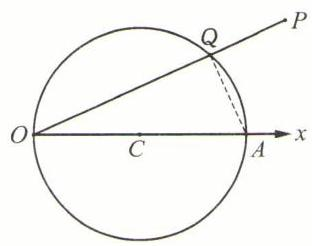
\includegraphics[width=0.2\textwidth]{bodyxb/src/bo_d20cdrf7aajc73bfmvhg_103_1113_349_312_246_0.jpg}
\end{center}


[第 49(2)题]

$\therefore {\rho }_{P} = {\rho }_{Q} - {10}\sin {\theta }_{P},\;\therefore$ 点 $P$ 的轨迹方程为 $\rho  = {10}\sqrt{2}\cos \left( {\theta  + \dfrac{\pi }{4}}\right) \left( {-\dfrac{\pi }{2} < \theta  \leq  0}\right)$ .

(3)圆 $M$ 的方程可整理为 ${\left( x - a\right) }^{2} + {y}^{2} = {b}^{2}$ . 题目中是先有切点 $N$ 和过点 $N$ 的切线, 再有点 $P$ . 事实上,完全可以先有过原点 $O$ ,倾斜角为 $\theta  \in  \lbrack 0,\pi )$ 的直线 ${l}_{1} : x\sin \theta  -$  $y\cos \theta  = 0$ ,再有与 ${l}_{1}$ 垂直的直线 $\left( \text{ 系 }\right) {l}_{2} : x\cos \theta  + y\sin \theta  + C = 0$ . 直线系中找到与圆 $M$ 相切的直线,也能得到切点 $N$ ,此时 ${l}_{1},{l}_{2}$ 交于点 $P.{l}_{2}$ 与圆 $M$ 相切的充要条件是 $\dfrac{\left| a\cos \theta  \pm  C\right| }{\sqrt{{\cos }^{2}\theta  + {\sin }^{2}\theta }} = b$ ,即 $C =  - a\cos \theta  \pm  b$ . 点 $P$ 的坐标可通过联立 ${l}_{1},{l}_{2}$ 求得,即 $\left\{  {\begin{array}{l} {x}_{P} =  - C \cdot  \cos \theta , \\  {y}_{P} =  - C \cdot  \sin \theta  \end{array}\left( \cdot \right) }\right.$ ,在以 $O$ 为极点,射线 ${Ox}$ 为极轴的极坐标系中,点 $P$ 的极角为 $\theta$ ,观察 (*) 式,不难看出点 $P$ 的极径是 $- C.\;\therefore \;$ 点 $P$ 轨迹的极坐标方程为 $\rho$  $= a\cos \theta  \pm  b\left( {\theta  \in  \lbrack 0,\pi }\right) )$ .

\begin{center}
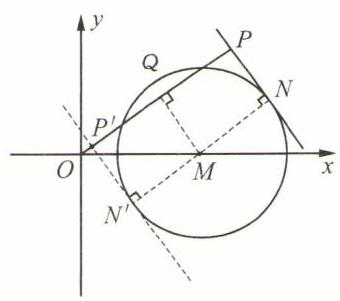
\includegraphics[width=0.2\textwidth]{bodyxb/src/bo_d20cdrf7aajc73bfmvhg_103_1083_782_340_301_0.jpg}
\end{center}


[第 49(3)题]

注:① 关于 $\theta$ 取值范围的拓展. $\because \left( {\rho ,\theta }\right)$ 和 $\left( {-\rho ,\theta  - \pi }\right)$ 代表同一点,若 $\theta  - \pi  \in  \lbrack 0,\pi )$ ,即 $\theta  \in  \lbrack \pi ,{2\pi })$ 时,有 $- \rho  =$  $a\cos \left( {\theta  - \pi }\right)  \pm  b$ ,即 $\rho  = a\cos \theta  \mp  b$ . 可见, $\rho  = a\cos \theta  \pm  b$ 在 $\theta  \in  \lbrack 0,{2\pi })$ 上均适用. 进一步, $\rho  = a\cos \theta  \pm  b$ 在 $\theta  \in  \mathbf{R}$ 上均适用. ②关于 $\rho  = a\cos \theta  \pm  b$ 的几何意义. 如图,连接 ${MN}$ ,作 ${MQ} \bot  {OP}$ 于点 $Q$ . $\left| {OQ}\right|  = a\cos \theta$ , $\left| {QP}\right|  = \left| {Q{P}^{\prime }}\right|  = b$ ,

$\therefore \left| {OP}\right|  = \left| {a\cos \theta  \pm  b}\right|$ . 需要说明的是,图中是 $a > b,\theta  \in  \left\lbrack  {0,\dfrac{\pi }{2}}\right)$ 的情况,而完整讨论所有情形,借助解析几何会更方便.

(4)以 $O$ 为原点,射线 ${OA}$ 为 $x$ 轴正方向,建立的直角坐标系中,有 $P\left( {r\cos \theta ,r\sin \theta }\right) ,A\left( {a,0}\right) ,O,B,P$ 三点共线,记 $\vv{OB}$  $= \lambda \vv{OP}$ ,故 $B\left( {{\lambda r}\cos \theta ,{\lambda r}\sin \theta }\right) ,\;\therefore \;\vv{AB} = \vv{OB} - \vv{OA} = \left( {{\lambda r}\cos \theta  - a,{\lambda r}\sin \theta }\right) ,\vv{AP} = \vv{OP} - \vv{OA} = \left( {r\cos \theta  - a,r\sin \theta }\right)$ , $\because \vv{AB}\bot \vv{AP}$ ,

$\therefore \vv{AB} \cdot  \vv{AP} = 0$ ,整理得 ${\lambda r}\left( {r - a\cos \theta }\right)  = a\left( {r\cos \theta  - a}\right) .\;\because$ 点 $A$ 在圆 $O$ 内,

$\therefore a < r,r - a\cos \theta  \neq  0,\therefore {\lambda r} = \dfrac{a\left( {a - r\cos \theta }\right) }{a\cos \theta  - r}$ . 观察点 $B$ 的直角坐标形式: $B\left( {{\lambda r}\cos \theta ,{\lambda r}\sin \theta }\right)$ ,不难看出,点 $B$ 的极角为 $\theta$ ,而极径为 $\rho  = {\lambda r}.\;\therefore$ 点 $B$ 的轨迹方程为 $\rho  = {\lambda r} = \dfrac{a\left( {a - r\cos \theta }\right) }{a\cos \theta  - r}$ .

50. (1) 若点 $P$ 的极坐标为 $\left( {{\rho }_{P},{\theta }_{P}}\right)$ ,则由已知,得点 $M$ 的极坐标为 $\left( {\dfrac{m}{m + n} \cdot  {\rho }_{P},{\theta }_{P}}\right)$ ,

$\therefore \;{\rho }_{M} = \dfrac{m}{m + n} \cdot  {\rho }_{P} = \dfrac{3m}{\left( {m + n}\right) \left( {\cos {\theta }_{P} - \sin {\theta }_{P}}\right) } = \dfrac{3m}{\left( {m + n}\right) \left( {\cos {\theta }_{M} - \sin {\theta }_{M}}\right) },$

\begin{center}
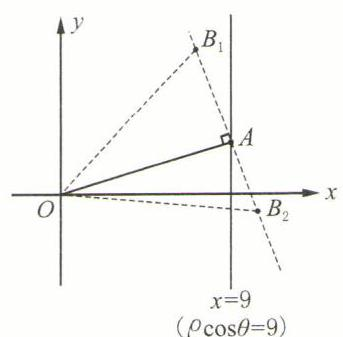
\includegraphics[width=0.2\textwidth]{bodyxb/src/bo_d20cdrf7aajc73bfmvhg_103_1083_1782_343_337_0.jpg}
\end{center}


[第 50(2)题]

$\therefore$ 点 $M$ 的轨迹方程为 $\rho  = \dfrac{3m}{\left( {m + n}\right) \left( {\cos \theta  - \sin \theta }\right) }$ .

(2)如图,若点 $A$ 的极坐标为 $\left( {{\rho }_{A},{\theta }_{A}}\right)$ ,不难写出点 $B$ 的极坐标与点 $A$ 之间的关系: $\left\{  \begin{array}{l} {\rho }_{B}\cos \dfrac{\pi }{6} = {\rho }_{A}, \\  {\theta }_{B} = {\theta }_{A} \pm  \dfrac{\pi }{6}. \end{array}\right.$ 又 ${\rho }_{A}\cos {\theta }_{A} = 9$ ,故 ${\rho }_{B} \cdot  \cos \dfrac{\pi }{6} \cdot  \cos \left( {{\theta }_{B} \pm  \dfrac{\pi }{6}}\right)  = 9,\;\therefore$ 点 $B$ 轨迹的极坐标方程为 $\rho \cos \left( {\theta  \pm  \dfrac{\pi }{6}}\right)  = 6\sqrt{3}\left( {\theta  \pm  \dfrac{\pi }{6} \neq  \dfrac{\pi }{2} + {k\pi },k \in  \mathbf{Z}}\right)$ . 注:尽管讨论的是

${\theta }_{A} \in  \left( {-\dfrac{\pi }{2},\dfrac{\pi }{2}}\right)$ 的情况,即 ${\theta }_{B} \mp  \dfrac{\pi }{6} \in  \left( {-\dfrac{\pi }{2},\dfrac{\pi }{2}}\right)$ 的情况,但使用本章 49(3) 注①的讨论方法, ${\theta }_{A}$ 的取值范围可以拓展到 ${\theta }_{A} \neq  \dfrac{\pi }{2} + {k\pi }\left( {k \in  \mathbf{Z}}\right)$ ,从而 ${\theta }_{B} \mp  \dfrac{\pi }{6} \neq  \dfrac{\pi }{2} + {k\pi }\left( {k \in  \mathbf{Z}}\right)$ 均可满足题意.

(3)如图,以 $A$ 为原点,射线 ${AB}$ 为 $x$ 轴正方向,建立平面直角坐标系,有 $A\left( {0,0}\right)$ , $B(a$ , 0 ). 圆 $B$ 的方程为 ${\left( x - a\right) }^{2} + {y}^{2} = {r}^{2}\left( {r < a}\right)$ . 以 $A$ 为极点,射线 ${AB}$ 为极轴建立极坐标系,此时圆 $B$ 的方程为 ${\left( \rho \cos \theta  - a\right) }^{2} + {\left( \rho \sin \theta \right) }^{2} = {r}^{2}$ ,即 ${\rho }^{2} - {2a\rho }\cos \theta  + {a}^{2} - {r}^{2} = 0$  $\left( *\right)$ . 若点 $P$ 的极坐标 $\left( {{\rho }_{P},{\theta }_{P}}\right)$ 满足 $\left( {}^{ * }\right)$ 式,而点 $Q$ 与点 $P$ 有如下关系:

\begin{center}
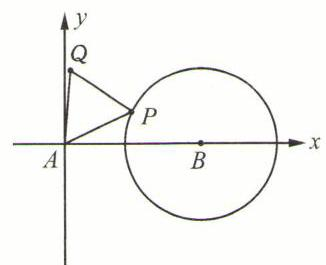
\includegraphics[width=0.2\textwidth]{bodyxb/src/bo_d20cdrf7aajc73bfmvhg_104_1200_262_326_265_0.jpg}
\end{center}


[第 50(3)题]

$\left\{  {\begin{array}{l} {\rho }_{Q} = {\rho }_{P}, \\  {\theta }_{Q} = {\theta }_{P} + \dfrac{\pi }{3}, \end{array}\;\therefore \;{\rho }_{Q}^{2} - {2a}{\rho }_{Q}\cos \left( {{\theta }_{Q} - \dfrac{\pi }{3}}\right)  + {a}^{2} - {r}^{2} = 0,}\right.$

$\therefore$ 点 $Q$ 的轨迹方程为 ${\rho }^{2} - {2a\rho }\cos \left( {\theta  - \dfrac{\pi }{3}}\right)  + {a}^{2} - {r}^{2} = 0$ .

(4)圆的极坐标方程为 ${13}{\rho }^{2} - {15\rho }\cos \theta  - {36\rho }\sin \theta  = 0.\because \rho$ 不恒为 0, $\therefore {13\rho } - {15}\cos \theta  - {36}\sin \theta  = 0\left( \star \right)$ (包含 $\rho  = 0$ 的情况). 若点 $M$ 的极坐标 $\left( {{\rho }_{M},{\theta }_{M}}\right)$ 满足 $\left( *\right)$ 式,而点 $N$ 与点 $M$ 又有如下关系 $\left\{  {\begin{array}{l} {\rho }_{N} \cdot  {\rho }_{M} = {12}, \\  {\theta }_{N} = {\theta }_{M}, \end{array}\;\therefore \;{13} \cdot  \dfrac{12}{{\rho }_{N}} - }\right.$  ${15}\cos {\theta }_{N} - {36}\sin {\theta }_{N} = 0,\therefore$ 点 $N$ 的轨迹的极坐标方程为 ${52} - {5\rho }\cos \theta  - {12\rho }\sin \theta  = 0$ ,其直角坐标形式为 ${5x} + {12y} -$  ${52} = 0.$

51. $C$ 提示: $\rho  = \dfrac{4}{2 - \lambda \cos \theta } = \dfrac{2}{1 - \dfrac{\lambda }{2}\cos \theta }$ ,当离心率 $e = \dfrac{\lambda }{2} \in  \left( {0,1}\right)$ ,即 $0 < \lambda  < 2$ 时,表示的是椭圆方程.

52. C 提示: ${\theta }_{1} = 0$ 时, ${\rho }_{1} = 5;{\theta }_{2} = \pi$ 时, ${\rho }_{2} = 1$ . $\therefore$ 长轴 ${2a} = {\rho }_{1} + {\rho }_{2} = 6,a = 3$ . 又 $\rho  = \dfrac{5}{3 - 2\cos \theta } = \dfrac{\dfrac{5}{3}}{1 - \dfrac{2}{3}\cos \theta },\therefore e = \dfrac{2}{3}$  $= \dfrac{c}{a} \Rightarrow  c = 2,b = \sqrt{{a}^{2} - {c}^{2}} = \sqrt{5}.\;\therefore \;$ 短轴长 $= {2b} = 2\sqrt{5}$ .

注: 也可由 $e = \dfrac{c}{a} = \dfrac{2}{3},p = \dfrac{{b}^{2}}{c} = \dfrac{5}{2},{c}^{2} = {a}^{2} - {b}^{2}$ 三式求得 $a = 3,b = \sqrt{5},c = 2$ ,进而短轴长 $= {2b} = 2\sqrt{5}$ .

53. B 提示: $\rho  = \dfrac{5}{3 - 2\cos \theta } = \dfrac{\dfrac{5}{3}}{1 - \dfrac{2}{3}\cos \theta }$ ,该曲线是椭圆. 又 $e = \dfrac{2}{3},{ep} = \dfrac{5}{3},\therefore p = \dfrac{5}{2},p$ 的含义即焦点到相应的准线的距离. 注:一定要将圆锥曲线先化为 $\rho  = \dfrac{ep}{1 - e\cos \theta }$ 的形式,即分母上的常数项为 1 .

54. C 提示: $e = \dfrac{1}{2}$ ,故曲线是椭圆. ${\theta }_{1} = 0$ 时, ${\rho }_{1} = 3;{\theta }_{2} = \pi$ 时, ${\rho }_{2} = 1,\;\therefore$ 长轴 $= {2a} = {\rho }_{1} + {\rho }_{2} = 4,a = 2$ . 曲线中心的直角坐标为 $\left( {a - {\rho }_{2},0}\right)$ ,即(1,0). 过该点与极轴垂直的直线方程的直角坐标形式为 $x = 1$ ,其极坐标形式为 $\rho \cos \theta  = 1$ .

55. D 提示: $\rho  = \dfrac{9}{4 - 5\cos \theta } = \dfrac{\dfrac{9}{4}}{1 - \dfrac{5}{4}\cos \theta }$ ,该曲线是双曲线. 方法一: 双曲线右焦点极坐标为极点(0,0).

\begin{center}
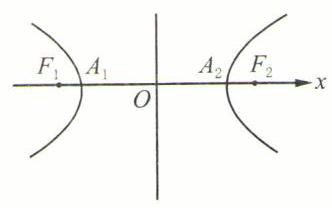
\includegraphics[width=0.2\textwidth]{bodyxb/src/bo_d20cdrf7aajc73bfmvhg_104_1200_1532_332_208_0.jpg}
\end{center}


(第 55 题)

又 $\left\{  \begin{array}{l} e = \dfrac{c}{a} = \dfrac{5}{4}, \\  p = \dfrac{{b}^{2}}{c} = \dfrac{9}{5}, \\  {c}^{2} = {a}^{2} + {b}^{2}, \end{array}\right.$ 解得 $\left\{  \begin{array}{l} a = 4, \\  b = 3, \\  c = 5. \end{array}\right. \therefore \;$ 左焦点极坐标为 $\left( {{2c},\pi }\right)$ ,即 $\left( {{10},\pi }\right)$ .

方法二: ${\theta }_{1} = 0$ 时, ${\rho }_{1} =  - 9;{\theta }_{2} = \pi$ 时, ${\rho }_{2} = 1$ ,如图,双曲线左、右焦点分别为 ${F}_{1},{F}_{2}$ ; 左、右顶点分别为 ${A}_{1},{A}_{2}$ ,则 $\left| {{F}_{1}{F}_{2}}\right|$  $= \left| {{F}_{1}{A}_{1}}\right|  + \left| {{A}_{1}{F}_{2}}\right|  = \left| {{F}_{2}{A}_{2}}\right|  + \left| {{A}_{1}{F}_{2}}\right|  = \left| {\rho }_{2}\right|  + \left| {\rho }_{1}\right|  = {10},\therefore$ 焦点坐标为(0,0)和 $\left( {{10},\pi }\right)$ .

56. D 提示: 方法一: 曲线为双曲线, $\left\{  {\begin{array}{l} e = \dfrac{c}{a} = 2, \\  p = \dfrac{{b}^{2}}{c} = \dfrac{1}{2}, \\  {c}^{2} = {a}^{2} + {b}^{2}. \end{array}\text{ 解得: }\left\{  {\begin{array}{l} a = \dfrac{1}{3}, \\  b = \dfrac{\sqrt{3}}{3}, \\  c = \dfrac{2}{3}, \end{array}\;\therefore \;\text{ 曲线中心坐标为 }\left( {-\dfrac{2}{3},0 + 2{k}_{1}\pi }\right) \text{ 或 }}\right. }\right.$  $\left( {\dfrac{2}{3},\pi  + 2{k}_{2}\pi }\right) \left( {{k}_{1},{k}_{2} \in  \mathbf{Z}}\right)$ . 对比选项,只有 $\left( {\dfrac{2}{3},\pi }\right)$ 符合.

方法二: 曲线为双曲线, ${\theta }_{1} = 0$ 时, ${\rho }_{1} =  - 1;{\theta }_{2} = \pi$ 时, ${\rho }_{2} = \dfrac{1}{3}$ ,曲线中心到右焦点(0,0)的距离为 $\dfrac{\left| {\rho }_{1}\right|  + \left| {\rho }_{2}\right| }{2} = \dfrac{2}{3}$ .

$\therefore$ 曲线中心坐标为 $\left( {-\dfrac{2}{3},0 + 2{k}_{1}\pi }\right)$ 或 $\left( {\dfrac{2}{3},\pi  + 2{k}_{2}\pi }\right) \left( {{k}_{1},{k}_{2} \in  \mathbf{Z}}\right)$ . 对比选项,只有 $\left( {\dfrac{2}{3},\pi }\right)$ 符合.

57. D 提示: 离心率 $e = \dfrac{2k}{{k}^{2} + 1}$ ,又 $k > 0,\therefore e = \dfrac{2}{k + \dfrac{1}{k}} \in  (0,1\rbrack ,\therefore$ 原极坐标方程表示的是椭圆 $\left( {0 < e < 1}\right)$ 或抛物线 $\left( {e = 1\text{ ,此时 }k = 1}\right)$ .

58. B 提示:由题意, $e = \dfrac{{C}_{n}^{2}}{6} = \dfrac{n\left( {n - 1}\right) }{12}$ ,解不等式 0 < $\dfrac{n\left( {n - 1}\right) }{12} < 1$ ,解得 $n \in  \left( {-3,0}\right)  \cup  \left( {1,4}\right)$ . 又 $n \in  \mathbf{N},\therefore n = 2$ 或 3,对应 $e = \dfrac{1}{6}$ 或 $\dfrac{1}{2}$ .

59. $C$ 提示:方法一:解方程 $\left\{  \begin{array}{l} e = \dfrac{c}{a}, \\  p = \dfrac{{b}^{2}}{c}, \\  {c}^{2} = {a}^{2} - {b}^{2}, \end{array}\right.$ 解得 $\left\{  \begin{array}{l} a = \dfrac{ep}{1 - {e}^{2}}, \\  b = \dfrac{ep}{\sqrt{1 - {e}^{2}}}, \\  c = \dfrac{{e}^{2}p}{1 - {e}^{2}}, \end{array}\right. \;\therefore$ 椭圆的长轴 ${2a} = \dfrac{2ep}{1 - {e}^{2}}$ .

方法二: ${\theta }_{1} = 0$ 时, ${\rho }_{1} = \dfrac{ep}{1 - e};{\theta }_{2} = \pi$ 时, ${\rho }_{2} = \dfrac{ep}{1 + e}$ ,椭圆长轴为 ${\rho }_{1} + {\rho }_{2} = \dfrac{2ep}{1 - {e}^{2}}$ .

60. B 提示: ${\theta }_{1} = \dfrac{\pi }{3}$ 时, ${\rho }_{1} = \dfrac{2}{3 - 2\cos \dfrac{\pi }{3}} = 1;{\theta }_{2} = \dfrac{\pi }{3} + \pi$ 时, ${\rho }_{2} = \dfrac{2}{3 - 2\cos \dfrac{4\pi }{3}} = \dfrac{1}{2}$ ,因此 $\theta  = \dfrac{\pi }{3}\left( {\rho  \in  \mathbf{R}}\right)$ 被 $\rho  = \dfrac{2}{3 - 2\cos \theta }$  $\left( {e = \dfrac{2}{3}\text{ ,曲线为椭圆) 所截得的弦长等于 }{\rho }_{1} + {\rho }_{2} = \dfrac{3}{2}}\right)$ .

61. D 提示: $\rho \cos \theta  =  - 2$ 是 $\rho  = \dfrac{4}{3 - 2\cos \theta } = \dfrac{\dfrac{2}{3} \times  2}{1 - \dfrac{2}{3}\cos \theta }$ (椭圆)的左准线,故左焦点 (极点) 到左准线的距离为 2. 根据对称性, 右准线到极点的距离 $=$ 右准线到右焦点的距离 $+ {2c} = 2 + {2c},{2c}$ 是焦距. 由 $e = \dfrac{c}{a} = \dfrac{2}{3},p = \dfrac{{b}^{2}}{c} = 2,{c}^{2} = {a}^{2} - {b}^{2}$ ,易解得 $c$  $= \dfrac{8}{5}$ ,故另一条准线的极坐标方程为 $\rho \cos \theta  = 2 + {2c} = 2 + 2 \times  \dfrac{8}{5} = \dfrac{26}{5}$ .

62. (1) $\rho  = \dfrac{3}{1 - \cos \theta }$ 提示: 由题意,焦点到准线的距离为 $p = 3$ . 又 $e = 1$ ,故抛物线方程是 $\rho  = \dfrac{ep}{1 - e\cos \theta } = \dfrac{3}{1 - \cos \theta }$ .

(2) $\rho  = \dfrac{3}{2 - \cos \theta }$ 提示: 设椭圆的极坐标方程为 $\rho  = \dfrac{ep}{1 - e\cos \theta }$ ,代入 (3,0) 和 (1, $\pi$ ),得 $\left\{  \begin{array}{l} \dfrac{ep}{1 - e} = 3, \\  \dfrac{ep}{1 + e} = 1, \end{array}\right.$ 解得 $\left\{  \begin{array}{l} e = \dfrac{1}{2}, \\  p = 3, \end{array}\right.$  $\therefore \rho  = \dfrac{ep}{1 - e\cos \theta } = \dfrac{\dfrac{3}{2}}{1 - \dfrac{1}{2}\cos \theta } = \dfrac{3}{2 - \cos \theta }$ .

63. 思路:对于非抛物线的圆锥曲线 $\rho  = \dfrac{ep}{1 - e\cos \theta }$ ,当 ${\theta }_{1} = 0$ 时, ${\rho }_{1} = \dfrac{ep}{1 - e}$ ；当 ${\theta }_{2} = \pi$ 时, ${\rho }_{2} = \dfrac{ep}{1 + e}$ . $\left| {{\rho }_{1} + {\rho }_{2}}\right|  = \dfrac{2ep}{\left| 1 - {e}^{2}\right| } =$  $\dfrac{2 \cdot  \dfrac{c}{a} \cdot  \dfrac{{b}^{2}}{c}}{\left| 1 - \dfrac{{c}^{2}}{{a}^{2}}\right| } = {2a};\left| {{\rho }_{1} - {\rho }_{2}}\right|  = \dfrac{2{e}^{2}p}{\left| 1 - {e}^{2}\right| } = \dfrac{2p}{\left| \dfrac{1}{{e}^{2}} - 1\right| } = \dfrac{2 \cdot  \dfrac{{b}^{2}}{c}}{\left| \dfrac{{a}^{2}}{{c}^{2}} - 1\right| } = {2c};\left| {{\rho }_{1} \cdot  {\rho }_{2}}\right|  = \dfrac{{e}^{2}{p}^{2}}{\left| 1 - {e}^{2}\right| } = \dfrac{{p}^{2}}{\left| \dfrac{1}{{e}^{2}} - 1\right| } = \dfrac{\dfrac{{b}^{4}}{{c}^{2}}}{\left| \dfrac{{a}^{2}}{{c}^{2}} - 1\right| } = {b}^{2}.$  $\therefore a = \dfrac{1}{2}\left| {{\rho }_{1} + {\rho }_{2}}\right| ,b = \sqrt{\left| {\rho }_{1} \cdot  {\rho }_{2}\right| },c = \dfrac{1}{2}\left| {{\rho }_{1} - {\rho }_{2}}\right|$ . (1) 2 提示: ${\theta }_{1} = 0$ 时, ${\rho }_{1} = 4;{\theta }_{2} = \pi$ 时, ${\rho }_{2} = 2$ . 焦距 ${2c} = \left| {{\rho }_{1} - {\rho }_{2}}\right|  = 2$ . (2) $\dfrac{4}{5}\;{10}\;\dfrac{25}{2}$ 提示: $\rho  = \dfrac{9}{5 - 4\cos \theta } = \dfrac{\dfrac{9}{5}}{1 - \dfrac{4}{5}\cos \theta }$ ,故离心率 $e = \dfrac{4}{5}$ . ${\theta }_{1} = 0$ 时, ${\rho }_{1} = 9;{\theta }_{2} = \pi$ 时, ${\rho }_{2} = 1.\;\therefore$ 长轴长 ${2a}$

$= \left| {{\rho }_{1} + {\rho }_{2}}\right|  = {10}$ ,两准线间的距离 $= \dfrac{2{a}^{2}}{c} = \dfrac{{\left( 2a\right) }^{2}}{2c} = \dfrac{{\left| {\rho }_{1} + {\rho }_{2}\right| }^{2}}{\left| {\rho }_{1} - {\rho }_{2}\right| } = \dfrac{{10}^{2}}{8} = \dfrac{25}{2}$ .

(3) $\left( {\dfrac{6}{5},0}\right)$ 提示: ${\theta }_{1} = 0$ 时, ${\rho }_{1} = 3;{\theta }_{2} = \pi$ 时, ${\rho }_{2} = \dfrac{3}{5},\;\therefore \;c = \dfrac{1}{2}\left| {{\rho }_{1} - {\rho }_{2}}\right|  = \dfrac{6}{5}$ . 椭圆中心到焦点的距离为 $c = \dfrac{6}{5}$ ,极坐标为 $\left( {\dfrac{6}{5},0}\right)$ .

(4)左准线为 $\rho \cos \theta  =  - 6$ 右准线为 $\rho \cos \theta  = {10}$ 提示: $\rho  = \dfrac{6}{2 - \cos \theta } = \dfrac{\dfrac{1}{2} \cdot  6}{1 - \dfrac{1}{2}\cos \theta }$ ,即 $e = \dfrac{1}{2},p = 6$ . $p$ 代表的是(左)焦点到 (左) 准线的距离,同时左焦点也是极点,故椭圆的左准线为 $\rho \cos \theta  =  - 6$ . 又 ${\theta }_{1} = 0$ 时, ${\rho }_{1} = 6;{\theta }_{2} = \pi$ 时, ${\rho }_{2} = 2$ ,两准线间的距离为 $\dfrac{2{a}^{2}}{c} = \dfrac{{\left( 2a\right) }^{2}}{2c} = \dfrac{{\left| {\rho }_{1} + {\rho }_{2}\right| }^{2}}{\left| {\rho }_{1} - {\rho }_{2}\right| } = {16},\therefore$ 右准线为 $\rho \cos \theta  =  - 6 + {16} = {10}$ . (或根据对称性,左焦点到右准线的距离 $=$ 焦距 + 右焦点到右准线的距离 $= {2c} + p = \left| {{\rho }_{1} - {\rho }_{2}}\right|  + p = {10}$ ,也能得到右准线极坐标方程 $\rho \cos \theta  = {10}$ )

(5) $\dfrac{4}{3}$ 提示: ${\theta }_{1} = 0$ 时, ${\rho }_{1} = 1;{\theta }_{2} = \pi$ 时, ${\rho }_{2} = \dfrac{1}{3},\;\therefore a = \dfrac{1}{2}\left| {{\rho }_{1} + {\rho }_{2}}\right|  = \dfrac{2}{3};c = \dfrac{1}{2}\left| {{\rho }_{1} - {\rho }_{2}}\right|  = \dfrac{1}{3}$ ,椭圆中心到准线的距离 $= \dfrac{{a}^{2}}{c} = \dfrac{4}{3}$ .

(6)(0,0)和(6,0)提示: ${\theta }_{1} = 0$ 时, ${\rho }_{1} = 8;{\theta }_{2} = \pi$ 时, ${\rho }_{2} = 2,\therefore c = \dfrac{1}{2}\left| {{\rho }_{1} - {\rho }_{2}}\right|  = 3$ . 极坐标系中,椭圆的极坐标为 (0, $0)$ 和(2c,0),即(0,0)和(6,0).

(7) $\dfrac{\pi }{3}\;{\theta }_{1} = 0$ 时, ${\rho }_{1} =  - 2;{\theta }_{2} = \pi$ 时, ${\rho }_{2} = \dfrac{2}{3}$ . 双曲线两条渐近线的斜率是 $\pm  \dfrac{b}{a}$ ,即 $\pm  \dfrac{\sqrt{\left| {\rho }_{1} \cdot  {\rho }_{2}\right| }}{\dfrac{1}{2}\left| {{\rho }_{1} + {\rho }_{2}}\right| } =  \pm  \sqrt{3}.\;\therefore$ 两条渐近线所夹锐角 $= \pi  - 2 \cdot  \arctan \sqrt{3} = \dfrac{\pi }{3}$ .

(8) $\dfrac{6}{7}\;\dfrac{2\sqrt{7}}{7}$ 提示: ${\theta }_{1} = 0$ 时, ${\rho }_{1} =  - 1;{\theta }_{2} = \pi$ 时, ${\rho }_{2} = \dfrac{1}{7}$ . $\;\therefore$ 实轴长 ${2a} = \left| {{\rho }_{1} + {\rho }_{2}}\right|  = \dfrac{6}{7}$ ；虚轴长 ${2b} = 2\sqrt{\left| {\rho }_{1} \cdot  {\rho }_{2}\right| }$  $= \dfrac{2\sqrt{7}}{7}$ .

(9) $\left( {\dfrac{ep}{1 - e},0}\right)$ 和 $\left( {\dfrac{ep}{1 + e},\pi }\right)$ 提示: 令 $\theta  = 0$ ,有 $\rho  = \dfrac{ep}{1 - e}$ ; 令 $\theta  = \pi$ ,有 $\rho  = \dfrac{ep}{1 + e}$ . 故双曲线顶点的极坐标为 $\left( {\dfrac{ep}{1 - e},0}\right)$ 和 $\left( {\dfrac{ep}{1 + e},\pi }\right)$ .

(10) $\dfrac{1}{3}$ 提示: $\rho  = \dfrac{2}{3 - 3\cos \theta } = \dfrac{1 \times  \dfrac{2}{3}}{1 - \cos \theta }$ ,故 $p = \dfrac{2}{3}$ 是焦点到准线的距离,而焦点到顶点的距离为 $\dfrac{1}{2}p = \dfrac{1}{3}$ .

64. (1) ${\theta }_{1} = \dfrac{\pi }{4}$ 时, ${\rho }_{1} = \dfrac{2}{3 - \dfrac{\sqrt{2}}{2}};{\theta }_{2} = \dfrac{\pi }{4} + \pi$ 时, ${\rho }_{2} = \dfrac{2}{3 + \dfrac{\sqrt{2}}{2}}$ . 所求弦长 $= {\rho }_{1} + {\rho }_{2} = \dfrac{2 \times  2 \times  3}{9 - \dfrac{1}{2}} = \dfrac{24}{17}$ .

(2) ${\theta }_{1} = \dfrac{\pi }{3}$ 时, ${\rho }_{1} =  - 4;{\theta }_{2} = \dfrac{\pi }{3} + \pi$ 时, ${\rho }_{2} = \dfrac{4}{5}$ . 即所截得的弦的端点极坐标为 $\left( {-4,\dfrac{\pi }{3}}\right)$ 和 $\left( {\dfrac{4}{5},\dfrac{4\pi }{3}}\right)$ . 其中 $\left( {-4,\dfrac{\pi }{3}}\right)$ 也可写成 $\left( {4,\dfrac{4\pi }{3}}\right)$ ,故所截得的弦长为 $4 - \dfrac{4}{5} = \dfrac{16}{5}$ . 注:将 $\left( {\rho ,\theta }\right)$ 写成 $\rho  > 0,\theta  \in  \lbrack 0,{2\pi })$ 的形式,更容易在极坐标系中找到对应点的准确位置.

(3) 由题意, $\left| {OA}\right|  = \dfrac{3}{2 - \cos \dfrac{\pi }{4}} = \dfrac{3}{2 - \dfrac{\sqrt{2}}{2}},\left| {OC}\right|  = \dfrac{3}{2 - \cos \dfrac{3\pi }{4}} = \dfrac{3}{2 + \dfrac{\sqrt{2}}{2}},\therefore \left| {OB}\right|  = \dfrac{1}{2}\left( {\left| {OA}\right|  + \left| {OC}\right| }\right)  = \dfrac{1}{2} \times  \dfrac{3 \times  2 \times  2}{4 - \dfrac{1}{2}}$  $= \dfrac{12}{7}$ . 将 $\rho  = \dfrac{12}{7}$ 代入 $\rho  = \dfrac{3}{2 - \cos \theta }$ ,解得 $\cos \theta  = \dfrac{1}{4}$ . 又 $\theta  \in  \lbrack 0,{2\pi })$ ,故 $\theta  = \arccos \dfrac{1}{4}$ 或 $\theta  = {2\pi } - \arccos \dfrac{1}{4}.\;\therefore$ 点 $B$ 的极坐标为 $\left( {\dfrac{12}{7},\arccos \dfrac{1}{4}}\right)$ 或 $\left( {\dfrac{12}{7},{2\pi } - \arccos \dfrac{1}{4}}\right)$ .

(4) 由题意, $a = \dfrac{1}{2}\left| {{A}_{1}{A}_{2}}\right|  = 3,c = \dfrac{1}{2}\left| {{F}_{1}{F}_{2}}\right|  = 2\sqrt{2}$ ,故 $b = \sqrt{{a}^{2} - {c}^{2}} = 1$ . 以焦点 ${F}_{1}$ 为极点,射线 ${F}_{1}{F}_{2}$ 为极轴,建立极坐标,则椭圆方程的极坐标形式为 $\rho  = \dfrac{ep}{1 - e\cos \theta } = \dfrac{\dfrac{c}{a} \cdot  \dfrac{{b}^{2}}{c}}{1 - \dfrac{c}{a}\cos \theta } = \dfrac{1}{3 - 2\sqrt{2}\cos \theta }.\left| {MN}\right|  = \dfrac{1}{3 - 2\sqrt{2}\cos \alpha } +$

$\dfrac{1}{3 - 2\sqrt{2}\cos \left( {\pi  - \alpha }\right) } = \dfrac{6}{9 - 8{\cos }^{2}\alpha }$ . 又 $\left| {MN}\right|  = {2b} = 2,\;\therefore \;{\cos }^{2}\alpha  = \dfrac{3}{4}.\;\because \;\alpha  \in  \lbrack 0,\pi ),\;\therefore \;\alpha  = \dfrac{\pi }{6}$ 或 $\alpha  = \dfrac{5\pi }{6}$ .

(5) 由题意, $a = 3,b = 4$ ,故 $c = \sqrt{{a}^{2} + {b}^{2}} = 5,e = \dfrac{c}{a} = \dfrac{5}{3},p = \dfrac{{b}^{2}}{c} = \dfrac{16}{5}$ . 以右焦点为极点,射线 ${Ox}$ 为极轴建立的极坐标系中,双曲线方程为 $\rho  = \dfrac{\dfrac{5}{3} \times  \dfrac{16}{5}}{1 - \dfrac{5}{3}\cos \theta } = \dfrac{16}{3 - 5\cos \theta }\left( {\rho  \in  \mathbf{R}}\right) .{\theta }_{1} = \dfrac{\pi }{4}$ 时, ${\rho }_{1} = \dfrac{16}{3 - \dfrac{5}{\sqrt{2}}} < 0;{\theta }_{2} = \dfrac{\pi }{4} + \pi$ 时, ${\rho }_{2} = \dfrac{16}{3 + \dfrac{5}{\sqrt{2}}} > 0$ .

$\therefore$ 点 $A,B$ 的极坐标可以写为 $A\left( {{\rho }_{2},\dfrac{5\pi }{4}}\right) ,B\left( {-{\rho }_{1},\dfrac{5\pi }{4}}\right)$ ,弦 ${AB}$ 中点 $C$ 到右焦点的距离,即极径 ${\rho }_{C} =$  $\dfrac{1}{2}\left\lbrack  {{\rho }_{2} + \left( {-{\rho }_{1}}\right) }\right\rbrack  ,\;\therefore \;{\rho }_{C} = \dfrac{80}{7}\sqrt{2}$ .

(6)以 $F$ 为极点,射线 ${Fx}$ 为极轴,建立极坐标系. 设双曲线的极坐标方程为 $\rho  = \dfrac{ep}{1 - e\cos \theta }\left( {e > 1,\rho  > 0}\right)$ . 分别取 $\theta  = \dfrac{\pi }{2}$ 和 $\theta  = \dfrac{3\pi }{2}$ ,得 ${P}_{1}\left( {{ep},\dfrac{\pi }{2}}\right) ,{P}_{2}\left( {{ep},\dfrac{3\pi }{2}}\right) ,\therefore \left| {{P}_{1}{P}_{2}}\right|  = {2ep}$ . 设直线 ${P}_{3}F$ 的倾斜角为 $\varphi \left( {0 < \varphi  < \pi }\right)$ ,则 $\tan \varphi  =  \pm  \dfrac{b}{a}$ . 由对称性,只需讨论 $\tan \varphi  = \dfrac{b}{a}$ 的情形,此时, $\cos \varphi  = \dfrac{a}{\sqrt{{a}^{2} + {b}^{2}}} = \dfrac{a}{c} = \dfrac{1}{e}$ ,双曲线与直线 $\cos \varphi  = \dfrac{1}{e}\left( {\rho  > 0}\right)$ 的反向延长

线有交点 ${P}_{3}$ ,此时极角为 $\varphi  + \pi$ ,对应地, $\rho  = \dfrac{ep}{1 - e\cos \left( {\varphi  + \pi }\right) } = \dfrac{ep}{1 + e\cos \varphi } = \dfrac{1}{2}{ep}.\left| {{P}_{1}{P}_{2}}\right|  = 4\left| {{P}_{3}F}\right|$ ,证毕.

65. 以左焦点 $F$ 为极点,射线 ${FO}$ 为极轴,建立极坐标系. 如图,作 ${OD} \bot  {AB}$ 于点 $D,{OD}$ 是 $\bigtriangleup {AOB}$ 中 ${AB}$ 边上的高. 记点 $A$ 的极角为 $\varphi \left( {\varphi  \in  \lbrack 0,\pi }\right) )$ ,则点 $B$ 的极角为 $\varphi  + \pi$ ,且 $\left| {OD}\right|  = \left| {OF}\right|  \cdot  \sin \varphi  = c \cdot  \sin \varphi$ . 设椭圆的极坐标方程为 $\rho  = \dfrac{ep}{1 - e\cos \theta }$ ,由题意, $a = \dfrac{10}{2} = 5$ . $b = \dfrac{8}{2} = 4,\;\therefore c = \sqrt{{a}^{2} - {b}^{2}} = 3,e = \dfrac{c}{a} = \dfrac{3}{5},p = \dfrac{{b}^{2}}{c} = \dfrac{16}{3}$ . 点 $A,B$ 的极径分别为 ${\rho }_{A} =$  $\dfrac{ep}{1 - e\cos \varphi },{\rho }_{B} = \dfrac{ep}{1 + e\cos \varphi },\;\therefore \;\left| {AB}\right|  = {\rho }_{A} + {\rho }_{B} = \dfrac{2ep}{1 - {e}^{2}{\cos }^{2}\varphi } = 8$ ,代入 $e,p$ 的值,解得 ${\cos }^{2}\varphi  = \dfrac{5}{9},\;\therefore \;\sin \varphi  = \sqrt{1 - {\cos }^{2}\varphi } = \dfrac{2}{3},$

\begin{center}
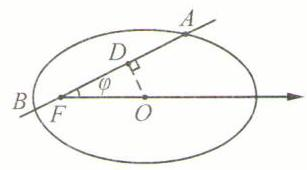
\includegraphics[width=0.2\textwidth]{bodyxb/src/bo_d20cdrf7aajc73bfmvhg_107_1118_852_307_170_0.jpg}
\end{center}


(第 65 题)

$\therefore {S}_{\bigtriangleup {AOB}} = \dfrac{1}{2} \cdot  \left| {AB}\right|  \cdot  \left| {OD}\right|  = \dfrac{1}{2} \cdot  8 \cdot  c\sin \varphi  = \dfrac{1}{2} \cdot  8 \cdot  3 \cdot  \dfrac{2}{3} = 8$ .

66. (1) 以焦点为极点, $x$ 轴正方向为极轴,建立的极坐标系中,抛物线的极坐标方程为 $\rho  = \dfrac{p}{1 - \cos \theta }$ . 设焦点弦的倾斜角 (极角) 为 $\varphi \left( {\varphi  \in  \left( {0,\pi }\right) }\right)$ ,则 $\dfrac{1}{a} + \dfrac{1}{b} = \dfrac{1 - \cos \varphi }{p} + \dfrac{1 - \cos \left( {\varphi  + \pi }\right) }{p} = \dfrac{2}{p}$ ,为定值,证毕.

(2)以圆锥曲线的焦点(椭圆为左焦点,双曲线为右焦点)为极点,垂直于焦点相应准线且指向背离于准线的方向为极轴,建立极坐标系,则圆锥曲线有统一的极坐标方程 $\rho  = \dfrac{ep}{1 - e\cos \theta }$ . 不妨设圆锥曲线的弦 $m$ 与极轴的夹角为 $\varphi$ (对于椭圆 $\varphi  \in  \left\lbrack  {0,\dfrac{\pi }{2}}\right)$ ; 对于抛物线和双曲线, $\varphi  \in  \left( {0,\dfrac{\pi }{2}}\right)$ . 弦长 ${l}_{1} = \dfrac{ep}{1 - e\cos \varphi } + \dfrac{ep}{1 - e\cos \left( {\varphi  + \pi }\right) } = \dfrac{2ep}{1 - {e}^{2}{\cos }^{2}\varphi }$ ,与弦 $m$ 垂直的弦 $n$ ,其弦长 ${l}_{2} = \dfrac{ep}{1 - e\cos \left( {\varphi  + \dfrac{\pi }{2}}\right) } + \dfrac{ep}{1 - e\cos \left( {\varphi  + \dfrac{3\pi }{2}}\right) } = \dfrac{2ep}{1 - {e}^{2}{\sin }^{2}\varphi }$ . $\therefore \;\dfrac{1}{{l}_{1}} + \dfrac{1}{{l}_{2}} = \dfrac{1 - {e}^{2}{\cos }^{2}\varphi }{2ep} +$  $\dfrac{1 - {e}^{2}{\sin }^{2}\varphi }{2ep} = \dfrac{2 - {e}^{2}}{2ep}$ ,为定值,证毕.

注: 由于椭圆的封闭性和抛物线仅有一支的特性,互相垂直的两条焦点弦倒数和恒为 $\dfrac{2 - {e}^{2}}{2ep}$ ,但对于双曲线,特别说明以下两点: ①双曲线互相垂直的两条焦点弦在同支时,必有 $2 - {e}^{2} > 0\left( {e < \sqrt{2}}\right)$ ,因为: 令 $\varphi  \in  \left( {0,\dfrac{\pi }{2}}\right)$ 使得 $\left\{  \begin{array}{l} 1 - e\cos \varphi  > 0, \\  1 - e\cos \left( {\varphi  + \dfrac{3}{2}\pi }\right)  > 0 \end{array}\right.$ 成立,即 $\sqrt{1 - \dfrac{1}{{e}^{2}}} < \sin \varphi  < \dfrac{1}{e}$ 在 $\varphi  \in  \left( {0,\dfrac{\pi }{2}}\right)$ 上有解, $\therefore \sqrt{1 - \dfrac{1}{{e}^{2}}} < \dfrac{1}{e}$ ,即 $1 < e < \sqrt{2}$ . ②如果不限定 “双曲线弦在同支”,讨论如下 $\left( {\varphi  \in  \left\lbrack  {0,\dfrac{\pi }{2}}\right) }\right)$ ；若弦 $m$ 端点在同支双曲线上,则 ${l}_{1} = \dfrac{2ep}{1 - {e}^{2}{\cos }^{2}\varphi }$ ；若弦 $m$ 端点不在同支双曲线上,则 ${l}_{1} =  - \dfrac{ep}{1 - e\cos \varphi } - \dfrac{ep}{1 - e\cos \left( {\varphi  + \pi }\right) } = \dfrac{-{2ep}}{1 - {e}^{2}{\cos }^{2}\varphi },\;\therefore \;{l}_{1} = \dfrac{2ep}{\left| 1 - {e}^{2}{\cos }^{2}\varphi \right| }$ . 同理, ${l}_{2} =$

$\dfrac{2ep}{\left| 1 - {e}^{2}{\sin }^{2}\varphi \right| }$ . $\therefore \;\dfrac{1}{{l}_{1}} + \dfrac{1}{{l}_{2}} = \dfrac{\left| {1 - {e}^{2}{\cos }^{2}\varphi }\right|  + \left| {1 - {e}^{2}{\sin }^{2}\varphi }\right| }{2ep}$ ,当且仅当 $\varphi$ 满足 $\left\{  \begin{array}{l} 1 - {e}^{2}{\cos }^{2}\varphi  > 0, \\  1 - {e}^{2}{\sin }^{2}\varphi  > 0 \end{array}\right.$ 或 $\left\{  \begin{array}{l} 1 - {e}^{2}{\cos }^{2}\varphi  < 0, \\  1 - {e}^{2}{\sin }^{2}\varphi  < 0 \end{array}\right.$ 时,即双曲线两弦的端点均在同支或均在两支时, $\dfrac{1}{{l}_{1}} + \dfrac{1}{{l}_{2}} = \dfrac{\left| 2 - {e}^{2}\right| }{2ep}$ 为定值. 若一条弦的端点在同支,而另一条弦的端点在两支上,则 $\dfrac{1}{{l}_{1}} + \dfrac{1}{{l}_{2}}$ 不为定值. 例如: 取 $e = 2,p = 1,\rho  = \dfrac{2}{1 - 2\cos \theta }$ ,取 $\theta  = 0,\pi$ ,得 ${l}_{1} = \dfrac{4}{3}$ (端点在两支上),取 $\theta  = \dfrac{\pi }{2},\dfrac{3\pi }{2}$ ,得 ${l}_{2} = 4$ (端点在同支上), $\dfrac{1}{{l}_{1}} + \dfrac{1}{{l}_{2}} = 1 \neq  \dfrac{\left| 2 - {e}^{2}\right| }{2ep} = \dfrac{1}{2}$ .

67. 方法一: 过 $P\left( {2,1}\right)$ 的参数方程为 $\left\{  \begin{array}{l} x = 2 + t\cos \alpha , \\  y = 1 + t\sin \alpha  \end{array}\right.$ ( $t$ 为参数, $\alpha  \in  \left( {\dfrac{\pi }{4},\pi }\right)$ ). 于是 $\dfrac{1}{\left| PQ\right| } = \sin \alpha  - \cos \alpha ,\dfrac{1}{\left| PM\right| } = \sin \alpha$ ,

$\therefore \dfrac{1}{\left| PQ\right| } + \dfrac{1}{\left| PM\right| } = \sin \alpha  - \cos \alpha  + \sin \alpha  = \sqrt{5}\sin \left( {\alpha  - \varphi }\right)$ (其中 $\varphi  = \arctan \dfrac{1}{2}$ ). 故当 $\alpha  = \dfrac{\pi }{2} + \arctan \dfrac{1}{2}$ ,即 $M\left( {{2.5},0}\right)$ 时, 有最大值为 $\sqrt{5}$ .

方法二: 设动点 $M$ 的坐标为 $M\left( {m,0}\right) \left( {m > 0}\right) ,{l}_{PM} : x + \left( {m - 2}\right) y - m = 0$ ,与 $y = x$ 交于点 $Q\left( {\dfrac{m}{m - 1},\dfrac{m}{m - 1}}\right) (m \neq  1$ ,否则 ${l}_{PM}$ 与 $y = x$ 平行). 又 ${x}_{Q} = \dfrac{m}{m - 1} > 0$ ,故 $m > 1.\left| {PQ}\right|  = \sqrt{{\left( \dfrac{m}{m - 1} - 2\right) }^{2} + {\left( \dfrac{m}{m - 1} - 1\right) }^{2}} = \dfrac{\sqrt{{m}^{2} - {4m} + 5}}{m - 1},\left| {PM}\right|  =$  $\sqrt{{\left( m - 2\right) }^{2} + {1}^{2}} = \sqrt{{m}^{2} - {4m} + 5},\;\therefore \;\dfrac{1}{\left| PM\right| } + \dfrac{1}{\left| PQ\right| } = \dfrac{m}{\sqrt{{m}^{2} - {4m} + 5}} = \dfrac{1}{\sqrt{5{\left( \dfrac{1}{m} - \dfrac{2}{5}\right) }^{2} + \dfrac{1}{5}}}$ . 当 $m = \dfrac{5}{2}$ 时,即 $M\left( {\dfrac{5}{2},0}\right)$ 时, $\dfrac{1}{\left| PM\right| } + \dfrac{1}{\left| PQ\right| }$ 有最大值 $\sqrt{5}$ .

68. 方法一: (参数方程法) 可设 $M\left( {a\cos \theta ,a\sin \theta }\right) ,P\left( {x,y}\right)$ ,则可得 $\left\{  \begin{array}{l} x = \dfrac{a\cos \theta }{1 + \cos \theta }, \\  y = \dfrac{a\sin \theta }{1 + \cos \theta } \end{array}\right.$ ( $\theta$ 为参数, $0 < \theta  < \dfrac{\pi }{2}$ ),消去 $\theta$ ,得点 $P$ 的轨迹的普通方程为 ${y}^{2} + {2ax} = {a}^{2}\;\left( {0 < x < \dfrac{a}{2}}\right)$ .

方法二: (极坐标法) 以点 $O$ 为极点,射线 ${Ox}$ 为极轴建立极坐标系,则点 $M$ 的极坐标可以写成 $\left( {{\rho }_{M},{\theta }_{M}}\right) \left( {{\theta }_{M} \in  \left( {0,\dfrac{\pi }{2}}\right) }\right.$ , 对应直角坐标为 $M\left( {{\rho }_{M}\cos {\theta }_{M},{\rho }_{M}\sin {\theta }_{M}}\right)$ . 在直角坐标系中, ${l}_{OM} : x\sin {\theta }_{M} - y\cos {\theta }_{M} = 0,{l}_{BL} : x\sin {\theta }_{M} + y - a\sin {\theta }_{M} = 0,{OM}$ , ${BL}$ 交点坐标为 $P\left( {\dfrac{a\cos {\theta }_{M}}{1 + \cos {\theta }_{M}},\dfrac{a\sin {\theta }_{M}}{1 + \cos {\theta }_{M}}}\right)$ ,

$\therefore {\rho }_{P} = \left| {OP}\right|  = \dfrac{a}{1 + \cos {\theta }_{M}} = \dfrac{a}{1 + \cos {\theta }_{P}}$ . 这就是点 $P$ 的极坐标方程,即 $\rho  + \rho \cos \theta  = a$ ,代入 $\rho  = \sqrt{{x}^{2} + {y}^{2}},\rho \cos \theta  = x$ ,则有点 $P$ 的直角坐标形式方程: ${y}^{2} + {2ax} = {a}^{2}\left( {0 < x < \dfrac{a}{2}}\right)$ .

69. 设两端点为 $A\left( {a,\dfrac{1}{a}}\right) ,B\left( {b,\dfrac{1}{b}}\right) ,{AB}$ 的中点为 $P\left( {x,y}\right)$ ,则 $\left\{  {\begin{array}{l} x = \dfrac{a + b}{2}, \\  y = \dfrac{1}{2}\left( {\dfrac{1}{a} + \dfrac{1}{b}}\right) , \end{array}\text{ 故 }\left\{  {\begin{array}{l} a + b = {2x}, \\  {ab} = \dfrac{x}{y} \end{array}\left( *\right) \text{ . (注: }x \neq  0}\right. }\right.$ ,否则 $a =$  $- b$ ,不能使 $\left| {AB}\right|  = 2$ ). 又 ${\left| AB\right| }^{2} = {\left( a - b\right) }^{2} + {\left( \dfrac{1}{a} - \dfrac{1}{b}\right) }^{2} = 4,\;\therefore \;{\left( a - b\right) }^{2}\left( {1 + \dfrac{1}{{a}^{2}{b}^{2}}}\right)  = 4$ ,

$\therefore \left\lbrack  {{\left( a + b\right) }^{2} - {4ab}}\right\rbrack   \cdot  \left( {1 + \dfrac{1}{{a}^{2}{b}^{2}}}\right)  = 4$ ,将 (*) 代入该式,整理得 $\left( {{x}^{2} + {y}^{2}}\right) \left( {{xy} - 1}\right)  = {xy}\left( {{xy} > 1}\right)$ .

注:点 $A,B$ 一定在双曲线 ${xy} = 1$ 的同一支上,说明如下: 若 ${ab} < 0$ ,不妨假定 $a > 0$ ,而 $b < 0$ . 令 $- b = {b}^{\prime } > 0$ ,则 ${\left| AB\right| }^{2} =$  ${\left( a + {b}^{\prime }\right) }^{2} + {\left( \dfrac{1}{a} + \dfrac{1}{{b}^{\prime }}\right) }^{2} = {a}^{2} + \dfrac{1}{{a}^{2}} + {b}^{\prime 2} + \dfrac{1}{{b}^{\prime 2}} + 2\left( {a{b}^{\prime } + \dfrac{1}{a{b}^{\prime }}}\right)  \geq  2 + 2 + 2 \cdot  2$ ,即 $\left| {AB}\right|  \geq  2\sqrt{2}$ ,当且仅当 $a = {b}^{\prime } = 1$ 时等号成立. 亦即: 若点 $A,B$ 位于双曲线 ${xy} = 1$ 的两支,那么 $\left| {AB}\right|$ 最小值为 $2\sqrt{2}$ ,不可能为 2 . 因此有 “ ${xy} > 1$ ”.

70. 方法一:将 $l$ 的参数方程 $\left\{  \begin{array}{l} x = t\cos \alpha , \\  y = a + t\sin \alpha  \end{array}\right.$ ( $t$ 为参数) 代入 $y = {x}^{2}$ ,得 ${t}^{2}{\cos }^{2}\alpha  - t\sin \alpha  - a = 0$ ,其两根为 ${t}_{1},{t}_{2}$ ,则 $k = \dfrac{1}{\left| {t}_{1}\right| } +$  $\dfrac{1}{\left| {t}_{2}\right| } = \dfrac{\sqrt{{\left( \left| {t}_{1}\right|  + \left| {t}_{2}\right| \right) }^{2}}}{\left| {t}_{1}{t}_{2}\right| } = \dfrac{1}{\left| {t}_{1}{t}_{2}\right| }\sqrt{{\left( {t}_{1} + {t}_{2}\right) }^{2} - 2{t}_{1}{t}_{2} + 2\left| {{t}_{1}{t}_{2}}\right| } = \dfrac{1}{\left| a\right| }\sqrt{{\sin }^{2}\alpha  + 2{\cos }^{2}\alpha \left( {a + \left| a\right| }\right) }$ . 于是若 $a < 0$ ,则 $k = \dfrac{1}{\left| a\right| }$

\begin{itemize}
\item $\left| {\sin \alpha }\right|$ ,显然与 $l$ 的倾斜角 $\alpha$ 有关,若 $a = 0$ ,则 $k$ 不存在,若 $a > 0$ ,则 $k = \dfrac{1}{\left| a\right| }\sqrt{{\sin }^{2}\alpha  + {4a}{\cos }^{2}\alpha } =$  $\dfrac{1}{a}\sqrt{1 + \left( {{4a} - 1}\right) {\cos }^{2}\alpha }$ ,显然,当 ${4a} - 1 = 0$ ,即 $a = \dfrac{1}{4}$ 时, $k$ 与 $\alpha$ 无关, $\therefore a = \dfrac{1}{4},k = 4$ .
\end{itemize}

方法二: $\because$ 直线 $l$ 与抛物线 $y = {x}^{2}$ 交于不同的两点, $\therefore$ 直线 $l$ 的斜率存在,设为 $m\left( {m \in  \mathbf{R}}\right) ,\therefore l : y = {mx} + a$ 与 $y = {x}^{2}$ 的交点满足 ${x}^{2} - {mx} - a = 0,\;\therefore \;{x}_{1} + {x}_{2} = m,{x}_{1}{x}_{2} =  - a.k = \dfrac{1}{\left| AP\right| } + \dfrac{1}{\left| AQ\right| } = \dfrac{1}{\sqrt{1 + {m}^{2}}}\left( {\dfrac{1}{\left| {x}_{1}\right| } + \dfrac{1}{\left| {x}_{2}\right| }}\right)  =$  $\dfrac{1}{\left| a\right| \sqrt{1 + {m}^{2}}}\left( {\left| {x}_{1}\right|  + \left| {x}_{2}\right| }\right)$ . 讨论: ①当 $a = 0$ 时, $\left| {AP}\right|$ 或 $\left| {AQ}\right|$ 为 0, $k$ 不存在,故 $a \neq  0$ . ② 当 $a < 0$ 时, ${x}_{1}{x}_{2} =  - a > 0$ ,故 ${x}_{1},{x}_{2}$ 同号, $k = \dfrac{1}{\left| a\right| \sqrt{1 + {m}^{2}}}\left( {\left| {x}_{1}\right|  + \left| {x}_{2}\right| }\right)  =  - \dfrac{\left| m\right| }{a\sqrt{1 + {m}^{2}}}$ ,随 $m$ 的变化而变化. ③当 $a > 0$ 时, ${x}_{1}{x}_{2} =  - a < 0$ ,故 ${x}_{1}$ , ${x}_{2}$ 异号, $k = \dfrac{1}{\left| a\right| \sqrt{1 + {m}^{2}}}\left( {\left| {x}_{1}\right|  + \left| {x}_{2}\right| }\right)  = \dfrac{\sqrt{{\left( {x}_{1} + {x}_{2}\right) }^{2} - 4{x}_{1}{x}_{2}}}{\left| a\right| \sqrt{1 + {m}^{2}}} = \dfrac{1}{a} \cdot  \sqrt{1 + \dfrac{{4a} - 1}{{m}^{2} + 1}}$ ,当且仅当 $a = \dfrac{1}{4}$ 时, $k$ 不随 $m$ 的变化而变化. 此时 $k = \dfrac{1}{a} = 4$ ,点 $A$ 是抛物线的焦点.

71. 方法一 (参数方程法): 把直线方程代入圆方程得 ${t}^{2} - {2ta}\cos \alpha  + {a}^{2} - {r}^{2} = 0$ . 记点 $A,B,P$ 所对应的参数分别为 ${t}_{1},{t}_{2},{t}_{3}$ . ① 当 $a > r > 0$ 时,由 $\dfrac{1}{\left| {t}_{1}\right| } + \dfrac{1}{\left| {t}_{2}\right| } = \dfrac{2}{\left| {t}_{3}\right| }$ ,得 $\left| {t}_{3}\right|  = \left| \dfrac{2{t}_{1}{t}_{2}}{{t}_{1} + {t}_{2}}\right|  = \left| \dfrac{{a}^{2} - {r}^{2}}{a\cos \alpha }\right|$ ,若点 $P$ 在圆内,则 $P\left( {\dfrac{{a}^{2} - {r}^{2}}{a},\dfrac{{a}^{2} - {r}^{2}}{a}\tan \alpha }\right)$ , 若点 $P$ 在圆外,则 $P\left( {-\dfrac{{a}^{2} - {r}^{2}}{a}, - \dfrac{{a}^{2} - {r}^{2}}{a}\tan \alpha }\right)$ ;

② 当 $r > a > 0$ 时,由 $\dfrac{1}{\left| {t}_{1}\right| } + \dfrac{1}{\left| {t}_{2}\right| } = \dfrac{2}{\left| {t}_{3}\right| }$ ,得 $\left| {t}_{3}\right|  = \dfrac{2\left| {{t}_{1}{t}_{2}}\right| }{\left| {t}_{1}\right|  + \left| {t}_{2}\right| } = \dfrac{-2{t}_{1}{t}_{2}}{\left| {t}_{1} - {t}_{2}\right| } = \dfrac{{r}^{2} - {a}^{2}}{\sqrt{{r}^{2} - {a}^{2}{\sin }^{2}\alpha }}$ ,故点 $P$ 坐标为 $\left( {\pm \dfrac{\left( {{r}^{2} - {a}^{2}}\right) \cos \alpha }{\sqrt{{r}^{2} - {a}^{2}{\sin }^{2}\alpha }}, \pm  \dfrac{\left( {{r}^{2} - {a}^{2}}\right) \sin \alpha }{\sqrt{{r}^{2} - {a}^{2}{\sin }^{2}\alpha }}}\right)$ ,对于 $a < 0$ ,也分为原点在圆外和原点在圆内类似地求解.

方法二: (极坐标法) 以原点 $O$ 为极点,射线 ${Ox}$ 为极轴建立极坐标系,此时直线 $l$ 的方程为 $l : \theta  = \alpha$ . 圆的方程为 ${\rho }^{2} -$  ${2a\rho }\cos \theta  + \left( {{a}^{2} - {r}^{2}}\right)  = 0$ ,代入 $\theta  = \alpha$ ,有 ${\rho }^{2} - {2a\rho }\cos \alpha  + \left( {{a}^{2} - {r}^{2}}\right)  = 0$ . $\Delta  > 0$ 时, ${\rho }_{1} + {\rho }_{2} = {2a}\cos \alpha ,{\rho }_{1} \cdot  {\rho }_{2} = {a}^{2} - {r}^{2}$ . 由题意,极径的倒数存在,故 $\rho  \neq  0 \Rightarrow  {a}^{2} \neq  {r}^{2}$ . 由 $\dfrac{1}{\left| OA\right| } + \dfrac{1}{\left| OB\right| } = \dfrac{2}{\left| OP\right| }$ ,可得 $\left| {\rho }_{P}\right|  = \dfrac{2\left| {{\rho }_{1} \cdot  {\rho }_{2}}\right| }{\left| {\rho }_{1} + {\rho }_{2}\right| }$ . 讨论: ①若 ${a}^{2} - {r}^{2} > 0$ ,则 ${\rho }_{1},{\rho }_{2}$ 同号, $\left| {\rho }_{1}\right|  + \left| {\rho }_{2}\right|  = \left| {{\rho }_{1} + {\rho }_{2}}\right| ,\;\therefore \;\left| {\rho }_{P}\right|  = \dfrac{2\left| {{a}^{2} - {r}^{2}}\right| }{2\left| a\right|  \cdot  \left| {\cos \alpha }\right| } = \dfrac{{a}^{2} - {r}^{2}}{\left| a\right|  \cdot  \left| {\cos \alpha }\right| },\;\therefore \;{\rho }_{P} =  \pm  \dfrac{{a}^{2} - {r}^{2}}{\left| a\right|  \cdot  \left| {\cos \alpha }\right| } =  \pm  \dfrac{{a}^{2} - {r}^{2}}{\left| a\right|  \cdot  \cos \alpha }$ , 点 $P$ 的极坐标为 $\left( {{\rho }_{P},\alpha }\right)$ ,故点 $P$ 的直角坐标为 $P\left( {\pm \dfrac{{a}^{2} - {r}^{2}}{\left| a\right| }, \pm  \dfrac{{a}^{2} - {r}^{2}}{\left| a\right| } \cdot  \tan \alpha }\right)$ (因为有 “ $\pm$ ” 符号,故也可简写成 $\left. {P\left( {\pm \dfrac{{a}^{2} - {r}^{2}}{a}, \pm  \dfrac{{a}^{2} - {r}^{2}}{a} \cdot  \tan \alpha }\right) }\right)$ . ②若 ${a}^{2} - {r}^{2} < 0$ ,则 ${\rho }_{1},{\rho }_{2}$ 异号, $\left| {\rho }_{1}\right|  + \left| {\rho }_{2}\right|  = \left| {{\rho }_{1} - {\rho }_{2}}\right|  = \sqrt{{\left( {\rho }_{1} + {\rho }_{2}\right) }^{2} - 4{\rho }_{1} \cdot  {\rho }_{2}}$ ,

$\therefore \left| {\rho }_{P}\right|  = \dfrac{2\left| {{a}^{2} - {r}^{2}}\right| }{\sqrt{4{a}^{2}{\cos }^{2}\alpha  - 4\left( {{a}^{2} - {r}^{2}}\right) }} = \dfrac{{r}^{2} - {a}^{2}}{\sqrt{{r}^{2} - {a}^{2}{\sin }^{2}\alpha }}$ ,点 $P$ 的极坐标为 $\left( {{\rho }_{P},\alpha }\right)$ ,故点 $P$ 的直角坐标为 $P\left( {\pm \dfrac{{r}^{2} - {a}^{2}}{\sqrt{{r}^{2} - {a}^{2}{\sin }^{2}\alpha }} \cdot  \cos \alpha , \pm  \dfrac{{r}^{2} - {a}^{2}}{\sqrt{{r}^{2} - {a}^{2}{\sin }^{2}\alpha }} \cdot  \sin \alpha }\right) .$

72. (1) 记椭圆的中心为 $A$ ,则 $\left\{  {\begin{array}{l} {x}_{A} = m, \\  {y}_{A} =  - m \end{array}\left( {m \in  \mathbf{R}}\right) }\right.$ . 消去参数 $m$ ,可得椭圆中心的轨迹方程为直线 $l : x + y = 0$ ,与 $m$ 无关, 证毕.

(2)平行于 $l$ 的直线方程可以写为 $y =  - x + b\left( {b \neq  0}\right)$ .

方法一: 将 $y =  - x + b$ 代入椭圆方程,整理得 $4{x}^{2} - \left( {{8m} + {6b}}\right) x + 4{m}^{2} + {6mb} + 3{b}^{2} - 3 = 0,\Delta  = {\left( 8m + 6b\right) }^{2} -$  ${16}\left( {4{m}^{2} + {6mb} + 3{b}^{2} - 3}\right)  = {48} - {12}{b}^{2} > 0,\therefore  - 2 < b < 2\left( {b \neq  0}\right)$ 时,直线 $y =  - x + b$ 与椭圆相交. 方法二: 将椭圆写成参数方程形式: $\left\{  {\begin{array}{l} x = m + \sqrt{3}\cos \theta , \\  y =  - m + \sin \theta  \end{array}\left( {\theta \text{ 是参数, }\theta  \in  \lbrack 0,{2\pi }))}\right. }\right.$ ,代入 $y =  - x + b$ ,得 $b = \sin \theta  + \sqrt{3}\cos \theta$  $= 2\sin \left( {\theta  + \dfrac{\pi }{3}}\right)$ . 直线与椭圆相交 $\Leftrightarrow$ 在 $\theta  \in  \lbrack 0,{2\pi })$ 上有且仅有两个相异的 $\theta$ 值满足三角方程 $b = 2\sin \left( {\theta  + \dfrac{\pi }{3}}\right)$ . $\therefore  - 2 < b < 2\left( {b \neq  0}\right)$ 时,直线 $y =  - x + b$ 与椭圆相交.

(3) 证法一: 承接前一问的方法一,弦长为 $\sqrt{{\left( {x}_{1} - {x}_{2}\right) }^{2} + {\left( {y}_{1} - {y}_{2}\right) }^{2}} = \sqrt{2} \cdot  \sqrt{{\left( {x}_{1} + {x}_{2}\right) }^{2} - 4{x}_{1}{x}_{2}} = \sqrt{2} \cdot  \dfrac{\sqrt{\Delta }}{4} =$  $\dfrac{1}{2}\sqrt{{24} - 6{b}^{2}}$ ,为定值且与 $m$ 的取值无关,证毕.

证法二: 承接前一问的方法二,弦长 $L$ 为 $\sqrt{{\left( {x}_{1} - {x}_{2}\right) }^{2} + {\left( {y}_{1} - {y}_{2}\right) }^{2}} = \sqrt{{\left( \sqrt{3}\cos {\theta }_{1} - \sqrt{3}\cos {\theta }_{2}\right) }^{2} + {\left( \sin {\theta }_{1} - \sin {\theta }_{2}\right) }^{2}}$ ,代

入 $b = \sin {\theta }_{i} + \sqrt{3}\cos {\theta }_{i}\left( {i = 1,2}\right)$ ,得 $L = \sqrt{2} \cdot  \sqrt{{\left( \sin {\theta }_{1} - \sin {\theta }_{2}\right) }^{2}}$ . 将 $b = \sin \theta  + \sqrt{3}\cos \theta$ 写成 ${\left( b - \sin \theta \right) }^{2} = 3\left( {1 - {\sin }^{2}\theta }\right)$ , 即关于 $\sin \theta$ 的方程: $4{\sin }^{2}\theta  - {2b}\sin \theta  + {b}^{2} - 3 = 0$ ,故弦长 $L = \sqrt{2} \cdot  \sqrt{{\left( \sin {\theta }_{1} - \sin {\theta }_{2}\right) }^{2}} = \sqrt{2} \cdot  \dfrac{\sqrt{\Delta }}{4} = \sqrt{2} \cdot  \dfrac{\sqrt{{48} - {12}{b}^{2}}}{4} =$  $\dfrac{1}{2}\sqrt{{24} - 6{b}^{2}}$ ,为定值且与 $m$ 的取值无关,证毕.

73. 椭圆方程整理得 $\dfrac{{\left( x - m\right) }^{2}}{5} + \dfrac{{\left( y - 2m\right) }^{2}}{4} = 1$ ,中心在直线 $y = {2x}$ 上,故所求直线可设为 $y = {2x} + t$ ,代入椭圆方程,整理得 ${24}{x}^{2} - \left( {{48m} - {2t}}\right) x + \left( {5{t}^{2} - {20mt} + {24}{m}^{2} - {20}}\right)  = 0$ . 弦长为 $\sqrt{5} \times  \dfrac{\sqrt{{80}\left( {{24} - {t}^{2}}\right) }}{24} = \dfrac{5\sqrt{3}}{3}$ ,解得 $t =  \pm  2\sqrt{3}$ ,故所求方程为 $l : y$  $= {2x} \pm  2\sqrt{3}.$

74. 证法一:以 $A$ 为极点,射线 ${AQ}$ 为极轴建立极坐标系. 记 ${OA} = a$ ,则圆 $O$ 的极坐标方程为 ${\rho }^{2} - {2a\rho }\cos \theta  + {a}^{2} - {R}^{2} = 0$ ,以 $\theta$  $= \dfrac{\pi }{4}$ 代入,得 ${\rho }^{2} - \sqrt{2}{\rho a} + {a}^{2} - {R}^{2} = 0$ ,其两根为 ${\rho }_{1},{\rho }_{2}$ ,于是 ${\left| AM\right| }^{2} + {\left| AN\right| }^{2} = {\left( {\rho }_{1} + {\rho }_{2}\right) }^{2} - 2{\rho }_{1}{\rho }_{2} = 2{R}^{2}$ . 同理可得 ${\left| BR\right| }^{2}$  $+ {\left| BS\right| }^{2} = 2{R}^{2}$ ,故左式 $\leq  \dfrac{{\left| AM\right| }^{2} + {\left| AN\right| }^{2} + {\left| BR\right| }^{2} + {\left| BS\right| }^{2}}{2} = 2{R}^{2}$ .

证法二: 以点 $O$ 为圆心,射线 ${OQ}$ 为 $x$ 轴正方向,建立平面直角坐标系,则圆 $O$ 的方程为 ${x}^{2} + {y}^{2} = {R}^{2}$ . 倾斜角为 ${45}^{ \circ  }$ 的直线系为 $l : y = x + m$ ,与 ${PQ}\left( {x\text{ 轴 }}\right)$ 交于点(-m,0),与圆 $O$ 交于点 $\left( {{x}_{1},{y}_{1}}\right) ,\left( {{x}_{2},{y}_{2}}\right)$ ,且满足: $2{x}^{2} + {2mx} + {m}^{2} - {R}^{2} = 0$ , 故 ${x}_{1} + {x}_{2} =  - m.\;\therefore {\left| AM\right| }^{2} + {\left| AN\right| }^{2} = {\left| BR\right| }^{2} + {\left| BS\right| }^{2} = {\left( {x}_{1} + m\right) }^{2} + {y}_{1}^{2} + {\left( {x}_{2} + m\right) }^{2} + {y}_{2}^{2} = 2{R}^{2} + 2{m}^{2} + {2m}\left( {x}_{1}\right.$  $\left. {+{x}_{2}}\right)  = 2{R}^{2}$ 为定值,与 $m$ 无关. $\therefore \left| {BR}\right|  \cdot  \left| {AM}\right|  + \left| {BS}\right|  \cdot  \left| {AN}\right|  \leq  \dfrac{{\left| BR\right| }^{2} + {\left| AM\right| }^{2} + {\left| BS\right| }^{2} + {\left| AN\right| }^{2}}{2} =$  $2{R}^{2}$ ,当且仅当 $\left| {BR}\right|  = \left| {AM}\right|$ 且 $\left| {BS}\right|  = \left| {AN}\right|$ (即点 $A,B$ 重合)时等号成立. 证毕.

$* {75}$ . 以椭圆中心 $O$ 为极点, $x$ 轴正向为极轴建立极坐标系,则椭圆的极坐标方程为 $\dfrac{{\rho }^{2}{\cos }^{2}\theta }{{a}^{2}} + \dfrac{{\rho }^{2}{\sin }^{2}\theta }{{b}^{2}} = 1,\therefore \dfrac{1}{{\rho }^{2}} = \dfrac{{\cos }^{2}\theta }{{a}^{2}} +$  $\dfrac{{\sin }^{2}\theta }{{b}^{2}} = \dfrac{1 + \cos {2\theta }}{2{a}^{2}} + \dfrac{1 - \cos {2\theta }}{2{b}^{2}}$ . 由题意,半径 ${r}_{1},{r}_{2},\cdots ,{r}_{n}$ 对应的极角可记为 $\varphi  + \dfrac{2\pi }{n} \cdot  1,\varphi  + \dfrac{2\pi }{n} \cdot  2,\cdots ,\varphi  + \dfrac{2\pi }{n} \cdot  n$ ,其中 $\varphi$ 是半径 ${r}_{n}$ 对应的极角. $\mathop{\sum }\limits_{{i = 1}}^{n}\dfrac{1}{{r}_{i}^{2}} = \mathop{\sum }\limits_{{i = 1}}^{n}\dfrac{1 + \cos \left( {{2\varphi } + \dfrac{4\pi }{n} \cdot  i}\right) }{2{a}^{2}} + \mathop{\sum }\limits_{{i = 1}}^{n}\dfrac{1 - \cos \left( {{2\varphi } + \dfrac{4\pi }{n} \cdot  i}\right) }{2{b}^{2}} = \dfrac{n}{2}\left( {\dfrac{1}{{a}^{2}} + \dfrac{1}{{b}^{2}}}\right)  + \left( {\dfrac{1}{2{a}^{2}} - \dfrac{1}{2{b}^{2}}}\right)$ . $\mathop{\sum }\limits_{{i = 1}}^{n}\cos \left( {{2\varphi } + \dfrac{4\pi }{n} \cdot  i}\right) .\;\because \;\cos \left( {{2\varphi } + \dfrac{4\pi }{n} \cdot  i}\right)  = \cos {2\varphi } \cdot  \cos \dfrac{4\pi i}{n} - \sin {2\varphi } \cdot  \sin \dfrac{4\pi i}{n},\;\therefore \;\mathop{\sum }\limits_{{i = 1}}^{n}\cos \left( {{2\varphi } + \dfrac{4\pi }{n} \cdot  i}\right)  = \cos {2\varphi } \cdot$  $\mathop{\sum }\limits_{{i = 1}}^{n}\cos \dfrac{4\pi i}{n} - \sin {2\varphi } \cdot  \mathop{\sum }\limits_{{i = 1}}^{n}\sin \dfrac{4\pi i}{n}$ . 下面,提供两种方法计算: $P = \mathop{\sum }\limits_{{i = 1}}^{n}\cos \dfrac{4\pi i}{n}$ 和 $Q = \mathop{\sum }\limits_{{i = 1}}^{n}\sin \dfrac{4\pi i}{n}$ . 方法一: 利用和差化积与积化和

差公式: $\mathop{\sum }\limits_{{i = 1}}^{n}\cos \left( {ix}\right)  = \dfrac{1}{\sin \dfrac{x}{2}} \cdot  \mathop{\sum }\limits_{{i = 1}}^{n}\cos \left( {ix}\right)  \cdot  \sin \dfrac{x}{2} = \dfrac{1}{2\sin \dfrac{x}{2}} \cdot  \mathop{\sum }\limits_{{i = 1}}^{n}\left\lbrack  {-\sin \left( {i - \dfrac{1}{2}}\right) x + \sin \left( {i + \dfrac{1}{2}}\right) x}\right\rbrack   = \dfrac{\sin \left( {n + \dfrac{1}{2}}\right) x - \sin \dfrac{1}{2}x}{2\sin \dfrac{x}{2}}$  $= \dfrac{\sin \dfrac{nx}{2} \cdot  \cos \dfrac{n + 1}{2}x}{\sin \dfrac{x}{2}}\left( {x \neq  {2k\pi },k \in  \mathbf{Z}}\right)$ . 同样, $\mathop{\sum }\limits_{{i = 1}}^{n}\sin \left( {ix}\right)  = \dfrac{1}{\sin \dfrac{x}{2}} \cdot  \mathop{\sum }\limits_{{i = 1}}^{n}\sin \left( {ix}\right)  \cdot  \sin \dfrac{x}{2} =  - \dfrac{1}{2\sin \dfrac{x}{2}}$ . $\mathop{\sum }\limits_{{i = 1}}^{n}\left\lbrack  {-\cos \left( {i - \dfrac{1}{2}}\right) x + \cos \left( {i + \dfrac{1}{2}}\right) x}\right\rbrack   =  - \dfrac{\cos \left( {n + \dfrac{1}{2}}\right) x - \cos \dfrac{1}{2}x}{2\sin \dfrac{x}{2}} = \dfrac{\sin \dfrac{n\pi }{2} \cdot  \sin \dfrac{n + 1}{2}x}{\sin \dfrac{x}{2}}\left( {x \neq  {2k\pi },k \in  \mathbf{Z}}\right)$ . 当 $x = {2k\pi }$  $\left( {k \in  \mathbf{Z}}\right)$ 时, $\mathop{\sum }\limits_{{i = 1}}^{n}\cos \left( {ix}\right)  = n,\mathop{\sum }\limits_{{i = 1}}^{n}\sin \left( {ix}\right)  = 0$ . 当 $n > 2$ 时, $\dfrac{4\pi }{n} \neq  {2k\pi }\left( {k \in  \mathbf{Z}}\right)$ ,代入 $x = \dfrac{4\pi }{n}$ ,得 $P = \mathop{\sum }\limits_{{i = 1}}^{n}\cos \left( {i \cdot  \dfrac{4\pi }{n}}\right)  = 0,Q =$  $\mathop{\sum }\limits_{{i = 1}}^{n}\sin \left( {i \cdot  \dfrac{4\pi }{n}}\right)  = 0$ . 方法二: 利用复数与三角的关系: 构造 $z = \cos \dfrac{4\pi }{n} + \mathrm{i} \cdot  \sin \dfrac{4\pi }{n}$ ( $\mathrm{i}$ 是虚数单位), $\therefore z + {z}^{2} + \cdots  + {z}^{n} =$  $P + \mathrm{i} \cdot  Q$ . 另一方面, $z + {z}^{2} + \cdots  + {z}^{n} = \dfrac{z\left( {1 - {z}^{n}}\right) }{1 - z}\left( {n > 2}\right)$ ,而 ${z}^{n} = \cos {4\pi } + \mathrm{i} \cdot  \sin {4\pi } = 1,\;\therefore z + {z}^{2} + \cdots  + {z}^{n} = 0$ . 根据复数相等的条件,得 $P = Q = 0\left( {n > 2}\right)$ . 由此, $\mathop{\sum }\limits_{{i = 1}}^{n}\cos \left( {{2\varphi } + \dfrac{4\pi }{n} \cdot  \mathrm{i}}\right)  = \cos {2\varphi } \cdot  P - \sin {2\varphi } \cdot  Q = 0,\;\therefore \;\mathop{\sum }\limits_{{i = 1}}^{n}\dfrac{1}{{r}_{i}^{2}} =$  $\dfrac{n}{2}\left( {\dfrac{1}{{a}^{2}} + \dfrac{1}{{b}^{2}}}\right) \left( {n > 2}\right)$ ,证毕. (注意: 无论 $\varphi$ 取何值,这个结论都成立).

